\documentclass[11pt,oneside]{book}
\usepackage[margin=1.2in]{geometry}
\usepackage{setspace}
\usepackage[toc,page]{appendix}
\usepackage{graphicx}
\usepackage{hyperref}
\usepackage{tabularx}
\usepackage{booktabs}
\usepackage{subcaption}
\usepackage{xcolor}  % For defining custom colors
\usepackage{fancyvrb}  % Enhanced verbatim environment
\usepackage{textcomp}
\definecolor{codegray}{gray}{0.95}  % Light gray color for code background

\newenvironment{code}{\VerbatimEnvironment
\begin{Verbatim}[frame=single, framerule=0pt, fillcolor=codegray, fillcolor=\color{codegray}]}{
\end{Verbatim}
}

\usepackage{listings} % Add this in your preamble
\usepackage{color}    % For syntax highlighting

\definecolor{codegreen}{rgb}{0,0.6,0}
\definecolor{codegray}{rgb}{0.5,0.5,0.5}
\definecolor{codepurple}{rgb}{0.58,0,0.82}
\definecolor{backcolour}{rgb}{0.95,0.95,0.92}

\lstdefinestyle{mystyle}{
    backgroundcolor=\color{backcolour},   
    commentstyle=\color{codegreen},
    keywordstyle=\color{magenta},
    numberstyle=\tiny\color{codegray},
    stringstyle=\color{codepurple},
    basicstyle=\ttfamily\footnotesize,
    breakatwhitespace=false,         
    breaklines=true,                 
    captionpos=b,                    
    keepspaces=true,                 
    numbers=left,                    
    numbersep=5pt,                  
    showspaces=false,                
    showstringspaces=false,
    showtabs=false,                  
    tabsize=2
}

\lstset{style=mystyle}


\usepackage[
backend=biber,
style=ieee,
sorting=none
]{biblatex}
\addbibresource{mybibliography.bib}


\usepackage{longtable} % Load the longtable package
\usepackage{array} % For defining new column types
\newcolumntype{Y}{>{\raggedright\arraybackslash}X}

\usepackage{pifont}
\usepackage{newunicodechar}
\newunicodechar{✓}{\ding{51}}
\newunicodechar{✗}{\ding{55}}
 
\begin{document}

\frontmatter

\begin{titlepage}

% You need to edit the details here

\begin{center}

\includegraphics[width=5cm]{images/UOSLogo_Portrait_Violet_RGB.png}\\[2cm]
\linespread{1.2}\huge {\bfseries VitalMonitor: IoT-driven Healthcare Management and Monitoring System}\\[2cm]
\linespread{1}
{\Large Vivek Vijay Choradia}\\[1cm]
{\large \emph{Supervisor:} Prof. Hamish Cunningham}\\[1cm]
\large \emph{A report submitted in fulfilment of the requirements}\\ \emph{for the degree of} BSc in Artificial Intelligence and Computer Science\\[0.3cm] 
\textit{in the}\\[0.3cm]
Department of Computer Science\\[2cm]
\today
\end{center}

\end{titlepage}

% -------------------------------------------------------------------
% Declaration
% -------------------------------------------------------------------

\newpage
\chapter*{\Large Declaration}

\setstretch{1.1} % set the line spacing differently if you wish, but this looks good to me. 

All sentences or passages quoted in this report from other people's work have been specifically acknowledged by clear cross-referencing to author, work and page(s). Any illustrations that are not the work of the author of this report have been used with the explicit permission of the originator and are specifically acknowledged. I understand that failure to do this amounts to plagiarism and will be considered grounds for failure in this project and the degree examination as a whole.\\[1cm]

\noindent Name: Vivek Vijay Choradia\\[1mm]
\rule[1em]{25em}{0.5pt}

\noindent Signature:\\[1mm]
\rule[1em]{25em}{0.5pt}

\noindent Date: \today\\[1mm] 
\rule[1em]{25em}{0.5pt}

% -------------------------------------------------------------------
% Abstract
% -------------------------------------------------------------------

\chapter*{\Large \center Abstract}

   % This research project explores the potential of non-intrusive wearable technologies in monitoring the health and well-being of healthcare professionals, specifically those working in high-stress environments such as operating theatres. The study is motivated by the critical need to ensure the health and safety of healthcare professionals, whose performance can directly impact patient outcomes. The project will investigate the feasibility of integrating wearable technologies, such as smart patches, into the existing attire of healthcare professionals. These devices, connected via the Internet of Things (IoT), could provide real-time monitoring of vital signs, enabling timely interventions if necessary. The research will address several challenges, including ensuring the accuracy and reliability of the devices, maintaining their non-intrusiveness, and addressing the well-being concerns of healthcare professionals. The project aims to contribute to the growing body of knowledge on wearable technologies in healthcare and highlight the potential of these technologies in improving patient care by ensuring the health and well-being of healthcare professionals. 

% This design and build project delves into the application of non-intrusive wearable technologies for monitoring the health and well-being of healthcare professionals, particularly in high-stress environments like operating theatres. It responds to the imperative of safeguarding the health and safety of these professionals, recognizing their direct influence on patient outcomes. The project centers on integrating wearable technologies seamlessly into healthcare attire. These devices, interconnected via the Internet of Things (IoT), offer real-time monitoring of vital signs, facilitating prompt interventions as needed. Emphasizing a proof-of-concept approach, the project will tackle challenges of ensuring device accuracy, reliability, and maintaining non-intrusiveness while prioritizing healthcare professionals' well-being. Significantly, it aims to develop a centralized solution for healthcare institutions, employing Smart Patch—an IoT device—to provide continuous real-time monitoring of vital signs for all healthcare professionals. This centralized system will display comprehensive data on a dashboard, enhancing situational awareness and enabling proactive healthcare interventions. This research aims not only to contribute to the expanding realm of wearable technologies in healthcare but also to underscore their potential in elevating patient care by ensuring the sustained health and well-being of healthcare professionals.


% This project introduces VitalMonitor, a tailored healthcare management and monitoring system for healthcare professionals through remote monitoring and non-intrusive design. By harnessing the power of Internet of Things (IoT) technology, VitalMonitor offers continuous, real-time monitoring of vital signs via Smart Patch - a wearable device. This system aims to elevate the vigilance and response capabilities of health institutions to their staff's well-being. The IoTaaS framework of VitalMonitor promises an all-in-one service, blending device and health data management smoothly; ensuring a seamless, integrated experience. With its core infrastructure, the project encapsulates a multifaceted approach—encouraging remote health supervision without imposing on the daily routines of healthcare professionals. The health data from the IoT device will feed directly into a web dashboard for each organization, presenting a clear, real-time view of staff health metrics. This centralized platform stands as a testament to the project's commitment to facilitating immediate and informed interventions, thereby preemptively addressing health concerns before they escalate. With VitalMonitor, the aim is to shift healthcare systems toward a more anticipatory and preventive stance, affirming the critical role of health monitoring in improving patient care by first ensuring the health of those who deliver it.  It underscores the indispensability of maintaining the health and well-being of healthcare professionals, ultimately reflecting an improved patient care environment.

% Project is on to make Internet of Things as a Service (IoTaaS) platform - VitalMonitor which is nothing but an IoT-driven Healthcare Management and Monitoring System for healthcare professionals (HCPs). When we talk about Healthcare it is always about the -patients and very less about HCPs. VitalMonitors offers continuous, real-time monitoring of vital signs via Smart Patch - a wearable IoT device. This system aims to elevate the vigilance and response capabilities of health institutions to their staff's well-being. 


% ADD WORDS LIKE CLOUD-BASED, ENCAPSULATES, ABSTRACTION, IOTAAS AND IOT BOTH, 
% This design and build project investigates the integration of non-intrusive wearable technologies—specifically Smart Patches—into the daily attire of healthcare professionals operating in high-stress environments, such as operating theatres. The initiative, named VitalMonitor, proposes an Internet of Things as a Service (IoTaaS) platform designed to provide continuous, real-time monitoring of vital signs. This technology aims to ensure the health and well-being of healthcare professionals, whose condition directly influences patient care outcomes. Challenges addressed in this study include ensuring the accuracy, reliability, and non-intrusiveness of the technology while maintaining user comfort and seamless integration into existing healthcare workflows. By developing a centralized dashboard for health data management, the project enables immediate interventions and proactive health monitoring, ultimately enhancing patient care by safeguarding the caregivers themselves. This research contributes to the body of knowledge on IoT applications in healthcare, emphasizing the critical role of wearable technologies in improving both healthcare delivery and professional well-being.

This design and build project develops VitalMonitor, an Internet of Things as a Service (IoTaaS) platform. VitalMonitor incorporates non-intrusive wearable IoT technology, specifically, Smart Patch —into the attire of healthcare professionals working in high-stress environments such as operating theaters. The platform aims to facilitate continuous and real-time monitoring of vital signs to ensure the health and safety of the professionals, thereby directly enhancing patient care outcomes. The research addresses challenges faced in accuracy, reliability, and seamless integration of these technologies into existing healthcare workflows. Through a centralized health data management dashboard and using messaging API, the system supports immediate interventions and proactive health monitoring. This study expands the knowledge base on IoT applications in healthcare, emphasizing the critical impact of wearable technologies on the improvement of healthcare service delivery and professional health.

\chapter*{\Large \center Acknowledgement}

I am profoundly grateful to my supervisor, Prof. Hamish Cunningham, for his invaluable guidance and inspiration throughout this project. His expertise in the Internet of Things, as demonstrated in the COM3505 module, significantly enhanced my understanding and passion for IoT applications in healthcare. I also extend my thanks to Gareth Coleman, the visiting academic for the module, whose practical insights were immensely helpful. \\

\noindent My appreciation goes to Dr. Matt Elis, my second marker, whose constructive feedback helped refine my work. Special thanks to the Electronics Lab team — Cecil Wilkinson and Dr. Tom Howard — whose patience and expertise were crucial in overcoming the technical challenges I faced. Additionally, I acknowledge the Department of Computer Science for providing the necessary facilities and resources. \\

\noindent A special thank you to Siya Pradhan, a dear friend whose support were invaluable during this journey. I will like to thank my sisters Mallika and Malvika, and my all my friends who believed in me and supported me throughout the dissertation journey.\\

\noindent And last but most importantly, I am also thankful to my parents for their endless encouragement and belief in my abilities. 

% -------------------------------------------------------------------
% TOC etc
% -------------------------------------------------------------------


\tableofcontents
\listoffigures
\listoftables
\lstlistoflistings

\setstretch{1.1} 

\mainmatter

\chapter{Introduction}

\section{Motivation}
Healthcare professionals (HCPs) are exposed to various sources of stress and pressure in their daily work, especially those who work in high-risk environments such as operation theatres. These stressors can negatively affect their physical, and mental health and well-being; as well as their performance and quality of care. Extensive research has been conducted on this topic indicating that HCPs are liable to experience a range of mental health issues, including depression \cite{ref1}, anxiety \cite{ref2}, burnout \cite{ref3}, and stress \cite{ref4}. A study which surveyed 3,700 public sector workers in the United Kingdom found that staff working for the National Health Service were the most stressed, with 61\% reporting feeling stress all or most of the time and as of 2015 59\% stating that stress has increased from previous years \cite{ref5}.\\

\noindent The well-being concerns for HCPs elevated during COVID-19 and after it. Multiple researches were undertaken around the world talking about anxiety, stress, depression and the psychological well-being of HCPs \cite{ref6}\cite{ref7}. This pressured healthcare institutions to work towards the health and well-being of their staff. More and more healthcare institutions worldwide are considering strategies for promoting staff safety and well-being. This project aims to create an Internet of Things as a Service (IoTaaS) Platform which helps these institutions get real-time insights into how to support HCPs in stressful environments best.


% \section{Aims and Objectives}

% The primary aim of this project is to delve into the potential of non-intrusive wearable technologies for real-time health monitoring of healthcare professionals, particularly those working in high-stress environments such as operating theatres, emergency rooms, and intensive care units. The motivation behind this aim is the critical need to ensure the health and well-being of these professionals, as their physical and mental state can directly impact the quality of care they provide to patients. \\

% The secondary aim of this project (which could also be labelled as future work)  is to open doors to further research opportunities that will elevate our current understanding of stressors in high-stress healthcare environments, and explore potential interventions to mitigate their impact. To reach that stage, a lot of potential work can be done following the creation of the device:

%  \begin{enumerate}
%      \item Conduct a feasibility study to evaluate the usability and acceptability of the prototype device among a sample of healthcare professionals working in high-stress environments, using surveys and interviews.
%      \item To analyse the data collected by the prototype device and assess the impact of the device on the health and well-being of healthcare professionals. This could involve statistical analysis of health indicators and correlation studies to understand the relationship between health indicators and stress and fatigue levels.
%      \item Based on the findings from the feasibility study and data analysis, provide recommendations and guidelines for the integration of non-intrusive wearable technologies into the existing attire of healthcare professionals and the improvement of their health and well-being. This could also include suggestions for improving HCPs' health and well-being based on the data analysis's insights.
%  \end{enumerate}

% \noindent If the timeframe of the project allows, the project will further dig into the above-mentioned works.

\section{Aims and Objectives}

The primary aim of this project is to design and implement VitalMonitor. VitalMonitor will be an integrated healthcare management system utilizing non-intrusive wearable technology for the real-time health monitoring of HCPs. This project targets professionals in high-stress environments, such as operating theatres and emergency rooms, where continuous health monitoring of the professionals is vital for maintaining high-quality patient care.\\

\noindent The objective would be to develop a wearable IoT device that measures vital without interfering with the HCPs' tasks, ensuring minimal disruption to their work. Additionally, the project will integrate this device within an Internet of Things as a Service (IoTaaS) platform, creating a seamless interface where health data is accessible in real-time through a web dashboard tailored for each healthcare institution.\\

\noindent With VitalMonitor, the project aspires to cultivate a proactive healthcare culture that consistently safeguards HCPs' welfare, establishing a foundation for improved patient care.


\section{Overview of the Report}
The introductory chapter establishes the foundation of this project, elucidating the motivation behind the study. It emphasizes the increasing awareness of healthcare professionals’ health and well-being. \\

\noindent\textbf{Chapter 2}, provides literature review for the project, discussing the current strategies used by healthcare institutions and their inefficiencies. This chapter also discusses how IoT and IoTaaS came into the scenario and brought different wearable technologies which helped in digitalising healthcare but still has no solution that could help HCPs. \\

\noindent\textbf{Chapter 3},  navigates essential aspects of the project - essentially what will be developed. It provides an overview of how the system will work, what features will be implemented and success metrics. This chapter concludes with the risks identified. \\

\noindent\textbf{Chapter 4},  establishes the technical aspects of the project. Provides insights into what technologies will be needed for the success of the project. This chapter also includes a comparative study between various technologies for each component of the project and choosing the most suitable one for the project. \\

\noindent\textbf{Chapter 5}, gives a high-level overview of VitalMonitor and its components. It also discusses alternative 
design approaches to some of the requirements defined in Chapter 3. Chapters 3, 4 and 5 combined represents what could be seen as a brief Software and Hardware Requirements Specification (SHRS) document of the system, providing a foundational blueprint for its development and implementation. \\

\noindent\textbf{Chapter 6}, outlines the processes involved in the implementation and subsequent testing of the VitalMonitor system. It covers the development of firmware, middleware, and the user dashboard, employing an agile methodology to ensure adaptability and responsiveness throughout the project lifecycle. This chapter also describes various testing methodologies employed to validate the functionality and reliability of the system to ensure that all components meet the predefined specifications and work cohesively.\\

\noindent\textbf{Chapter 7}, discusses the final outcomes of the VitalMonitor system, highlighting the achievements and the impact of the solution. It critically analyzes the main limitations encountered during the project and suggests potential areas for future improvements. The evaluation of the system's performance and the feasibility of its application in real-world settings are also thoroughly examined.\\

\noindent\textbf{Chapter 8}, concludes the report by revisiting how developing this platform would help healthcare professionals and summarising why the proposed platform has shown potential to be widely used, if introduced to the market. The chapter reflects on the contributions of the project to the field of healthcare technology and outlines future research directions that could further enhance the system's functionality and marketability.

\newpage
\chapter{Literature Review}

This chapter critically explores the existing frameworks and interventions employed by healthcare institutions to support the well-being of healthcare professionals (HCPs), examining their effectiveness and limitations. It reviews the impact of stress and fatigue on HCPs within healthcare settings and evaluates how these challenges are currently being addressed. The chapter also highlights the significant role that emerging technologies, particularly the Internet of Things (IoT) and IoT-as-a-Service (IoTaaS), can play in enhancing the monitoring and management of healthcare environments. Additionally, it considers the shortcomings of current wearable technologies in providing non-intrusive, real-time health monitoring in remote settings. The review aims to underscore the necessity for innovative solutions that cater more effectively to the needs of healthcare professionals, thereby improving their well-being and the overall quality of patient care.

\section{Stress and Fatigue}
\subsection{What is Stress?}
As per World Health Organization (WHO), Stress can be defined as a state of worry or mental tension caused by a difficult situation. Stress is a natural human response that prompts us to address challenges and threats in our lives. Everyone experiences stress to some degree. The way we respond to stress, however, makes a big difference to our overall well-being. Stress affects both the mind and the body. A little bit of stress is good and can help us perform daily activities. Too much stress can cause physical and mental health problems. \cite{48} 

\subsection{What is Fatigue?}
Fatigue is a term used to describe an overall feeling of tiredness or lack of energy. It isn’t the same as simply feeling drowsy or sleepy. When you’re fatigued, you have no motivation and no energy. Being sleepy may be a symptom of fatigue, but it’s not the same thing. \cite{49}

\subsection{Stress and Fatigue in Healthcare Settings}
Stress in healthcare professionals often stems from the high-pressure environment of medical settings, where the stakes are exceptionally high. Common stressors include long hours, complex patient interactions, and the emotional burden of continuous care giving. This chronic stress can lead to psychological symptoms such as anxiety and depression, and physical symptoms like headaches and hypertension, ultimately impacting their work efficacy and personal wellbeing. \\ 

Fatigue among healthcare professionals is more than just feeling tired; it’s a profound exhaustion that can result from prolonged physical, mental, and emotional labor. It is exacerbated by factors such as irregular shift patterns, the physical demands of the job, and the mental load of making critical decisions. Chronic fatigue can impair cognitive functions, reduce job performance, and increase the likelihood of errors in patient care. \\

\noindent In healthcare settings, stress and fatigue are exacerbated by the need to provide constant, high-quality care amidst frequently understaffed conditions. The relentless pace and emotional intensity of healthcare work can lead to burnout, a state of emotional, physical, and mental exhaustion. This not only affects the health of healthcare professionals but also compromises patient safety and the overall effectiveness of healthcare delivery.


\section{Current Strategies of Healthcare Institutions and their Inefficiencies}

The healthcare sector has been proactive in adopting various strategies to enhance the well-being of healthcare professionals (HCPs), acknowledging the multifaceted challenges they face. Despite the theoretical benefits of these strategies, practical inefficiencies and limitations often undermine their effectiveness.

\subsection{Integrated Care Systems (ICSs)}

Integrated Care Systems (ICSs) have been a cornerstone in the UK's healthcare strategy. ICSs are designed to facilitate cohesive planning and service delivery across various healthcare domains, including both physical and mental health services, as well as social care. The overarching goal is to enable individuals to lead healthier and more independent lives through self-care and prevention \cite{ref9}. However, ICSs sometimes struggle with delivering integrated care effectively, leading to fragmented services that are poorly coordinated around HCPs' needs. This fragmentation not only detracts from the patient and HCP experience but also results in inefficient resource use, echoing the financial and resource inefficiencies previously identified in Clinical Commissioning Groups (CCGs) \cite{ref11,ref12}.

\subsection{Understanding Evolving Needs}

The \textbf{Understanding Evolving Needs} strategy, informed by Accenture's survey of 720 healthcare providers, seeks to align healthcare institutions with the shifting expectations of HCPs, a need that became particularly acute during the COVID-19 pandemic \cite{ref18}. While this adaptive approach is commendable, accurately identifying and addressing the evolving needs of HCPs presents significant challenges, with effectiveness varying based on numerous factors including the healthcare setting and the specific needs of HCPs \cite{ref13,ref14}.

\subsection{Workplace Interventions}

\textbf{Workplace Interventions}, such as stress management programs, mindfulness practices, and workload adjustments, have been implemented to improve well-being and mitigate burnout among HCPs \cite{ref10}. Nonetheless, their effectiveness can be inconsistent, largely dependent on how well these interventions are tailored and executed within the unique contexts of different healthcare settings \cite{ref15}.

\subsection{Questionnaires}

The use of \textbf{Questionnaires} to assess the health and well-being of HCPs reflects a direct approach to understanding their needs. However, this method often fails to capture real-time changes and may elicit responses that do not accurately reflect the HCPs' health status \cite{ref16}. HCPs might prioritize patient care over their well-being or misjudge their health status as balanced, leading to responses that may not be entirely accurate or reflective of their actual needs. \\

\noindent The inefficiencies and limitations inherent in these strategies underscore the pressing need for innovative solutions that offer more immediate and comprehensive support for HCPs. One promising direction is the adoption of \textbf{Wearable Technologies}, an Internet of Things (IoT) application in healthcare, which could provide real-time health monitoring and personalized support, addressing many of the current methodologies' shortcomings.

\section{Measuring Stress and Fatigue Levels in Real-time}
Currently, there is no universally accepted algorithm for precisely calculating stress and fatigue levels, as these conditions are influenced by a complex interplay of physical, psychological, and environmental factors. This lack of a standardized measurement approach makes it challenging to accurately assess and manage stress and fatigue, particularly in high-pressure environments like healthcare settings.

% https://www.medicalnewstoday.com/articles/stress-measurement#normal-stress-levels

\subsection{Current Practices by state-of-the-art technologies}
Technological advancements have led to the development of devices that can measure indicators of stress in real-time. One notable example is the use of Electrodermal Activity (EDA) testing, popularized by devices like Fitbit. EDA measures the skin's electrical activity, which varies with the body’s sweat level— a physiological response associated with stress. Fitbit's implementation of this technology assesses stress levels by requiring users to engage in a two-minute meditation session, during which the device monitors changes in EDA. \cite{49} However, this method poses practical challenges for healthcare professionals (HCPs) who often cannot spare two uninterrupted minutes for such a test while on duty. Therefore, while valuable, this technology may not always be suitable for real-time stress monitoring in fast-paced healthcare environments.


\subsection{Next Best Alternative?}
To adapt real-time stress and fatigue monitoring for healthcare settings, technologies need to utilize parameters that can be passively monitored without disrupting workflow. These parameters should be trackable via remote and non-intrusive devices, allowing healthcare professionals (HCPs) to wear and use them continuously throughout their duties. By "non-intrusive," it means the device should be lightweight, comfortable, and not interfere with the user's regular activities or medical tasks.

Some of the key parameters that can be tracked to provide a viable alternative for a comprehensive stress or fatigue score include:

\begin{itemize}
    \item \textbf{Heart Rate Variability (HRV):} HRV is a useful indicator of the autonomic nervous system's balance and can reflect an individual's stress and recovery levels. Monitoring HRV continuously can provide real-time insights into the stress levels of HCPs, allowing for timely interventions.
    \item \textbf{Continuous EDA Monitoring:} Electrodermal activity, which reflects changes in the skin's conductance due to sweating, is a direct physiologic response to stress. By continuously monitoring EDA, devices can detect fluctuations in stress levels without requiring the user to engage in a specific task like meditation.
\end{itemize}

These paramaters/technologies should be integrated into devices that are easy to use and interpret, ensuring that HCPs can benefit from the insights provided without needing extensive training or causing disruption to their critical work. And one of the leading technologies which can help making such a device is Internet of Things.


\section{Internet of Things (IoT)}
The Internet of Things (IoT) describes the network of physical objects —``things”— that are embedded with sensors, software, and other technologies to connect and exchange data with other devices and systems over the Internet. These devices range from ordinary household objects to sophisticated industrial tools. With more than 7 billion connected IoT devices today, experts are expecting this number to grow to 22 billion by 2025. \cite{ref16}\\

While IoT has been in the tech industry for a a long time, only recent advances in several different technologies have made it practical and therefore popular. \\

IoT devices generate vast amounts of data - offering valuable insights for businesses and individuals. With advances in machine learning and analytics, coupled with IoT data, businesses can gather insights faster and more easily. The emergence of these allied technologies continues to push the boundaries of IoT and the data produced by IoT also feeds these technologies. \cite{ref16}

\section{IoT in Healthcare}
The Internet of Things (IoT) in healthcare, also known as the Internet of Medical Things (IoMT), refers to  it’s a network of medical devices, software, and tech solutions that can monitor patient health, manage treatments, and even assist in surgical procedures \cite{47}. These devices are equipped with internet connectivity, enabling them to communicate with healthcare systems and each other. This integration facilitates a broad spectrum of health services and medical applications. \\

IoMT encompasses a variety of devices from wearable health monitors to advanced surgical equipment. These tools collect, analyze, and transmit health data, providing real-time insights crucial for informed decision-making and tailored patient care. The use of IoMT leads to greater accuracy in diagnoses, improves treatment outcomes, and enhances the efficiency of healthcare operations.\\


% https://relevant.software/blog/iot-in-healthcare/#:~:text=IoT%20in%20healthcare%2C%20also%20known%20as%20IoMT%20solution,manage%20treatments%2C%20and%20even%20assist%20in%20surgical%20procedures.

\subsection{Wearables}

Wearables are electronic devices (IoT devices) that can be worn or carried on the body. These devices can be separated into categories such as smartwatches, wristbands, and hearables. The personal data of the user can be monitored and measured through powerful microchips and smart sensors that are embedded within the wearable device. Connecting to additional devices using Bluetooth, WiFi or a cellular network can further enhance the user experience \cite{ref17}. They are the most used device for healthcare monitoring. \\

\subsubsection{Smart Watch}
Smart watches stand out in the wearable technology landscape for their versatility and widespread adoption. As per Statista, 2023, smartwatches currently dominate the wearables market and have held a share of around 45 per cent since 2018. Most fitness trackers are built into smartwatches and can track steps, distance, heart rate, calories burnt, and other fitness metrics. They offer a comprehensive suite of features that go beyond fitness tracking to include notifications, apps, and sometimes even phone capabilities. Their appeal lies in their ability to provide a snapshot of an individual's health and daily activities directly from their wrist.

\subsubsection{Chest Strap}
Chest straps are specialized wearables designed for precise heart rate monitoring. Unlike wrist-based devices, chest straps measure electrical signals directly from the chest, offering a higher level of accuracy. They are particularly favored by athletes and individuals engaged in rigorous physical activities for monitoring heart rate and performance metrics.

\subsection{Limitations}
\subsubsection{Remoteness}
One significant limitation of current wearable technology is its remoteness or isolation from centralized healthcare systems. This disconnect hampers the potential for wearables to inform clinical decisions and provide a holistic view of a patient's health.

While wearable devices are capable of collecting a broad spectrum of health data from healthcare professionals themselves, there remains a significant barrier in integrating this data with the centralized systems used in hospitals and clinics. This is because most of such devices are made with general consumers in mind and the manufacturers don't usually sell it to organization with the perspective of monitoring health of all the staff in an organization. This disconnect hinders the ability of these devices to inform the organization about the health and fatigue levels of healthcare professionals in real time, which could otherwise support better staffing decisions and reduce the risk of burnout and medical errors.

\subsubsection{Non-Intrusiveness}

In healthcare settings, the non-intrusiveness of wearables is crucial. However, even state-of-the-art smartwatches face restrictions in sensitive environments like operation theatres or Intensive Care Units (ICUs). According to NHS England's guidance on uniforms and workwear, wearing watches in clinical settings is discouraged due to the risk of harboring microorganisms and hindering effective hand hygiene \cite{ref20}. Moreover, wristwatches may interfere with medical procedures, posing risks during surgeries or delicate operations.

\subsection{Why do Non-Intrusive devices don't exists in Healthcare?}
Healthcare devices are subject to rigorous regulatory scrutiny to ensure they meet high standards of accuracy, reliability, and safety. The certification process for medical devices, which includes clinical trials and detailed documentation, is both time-consuming and expensive. This rigorous scrutiny is essential to prevent errors that could directly affect patient health but creates a significant barrier to entry for new and innovative non-intrusive technologies. Furthermore, different countries and regions have their own regulatory frameworks, which can complicate the process for manufacturers looking to market their devices globally.\\

While non-intrusive devices offer the convenience of passive monitoring, maintaining the accuracy and reliability of these devices remains a technological hurdle. Sensor technology, particularly in non-intrusive formats, must evolve to capture data with the same precision as more traditional, intrusive methods. For example, sensors that work under or through clothing or that can monitor biometrics without direct skin contact often face issues such as signal attenuation or interference. These limitations can result in less reliable data, which in turn may affect the clinical utility of the information these devices provide.


\noindent Therefore, no such device exists which is remote and non-intrusive which can be used for monitoring vitals of healthcare professionals while they are working.

\section{Internt of Things as a Service (IoTaaS)}
Internet of Things-as-a-Service is one of the latest iterations in the "as-a-service" model that has become one of the popular technologies \cite{45}. IoTaaS, or IaaS, or Internet of Things as a Service, integrates IoT technology into a service model, allowing companies to use IoT solutions without managing the infrastructure. It became notably popular in the mid-2010s as businesses sought to enhance efficiency and data collection without the overhead of developing proprietary IoT systems. \\

\noindent IoTaaS has been a subject of extensive research and development, as evidenced by its frequent spotlight at the EAI International Conference on IoT as a Service and Consumer Electronics Showcase. The EAI IoTaaS 2024 conference, for instance, is set to highlight cutting-edge advancements in IoT technologies and their applications across various industries. These conferences serve as pivotal forums for exchanging ideas and fostering international collaboration among scholars and industry experts, thereby propelling the global IoT industry forward.\cite{46} 

\section{IoTaaS Platforms in Healthcare}
IoTaaS has become a transformative force in healthcare, enabling sophisticated remote patient monitoring systems and real-time data transmission to medical professionals. Such capabilities have improved the management of chronic diseases, improving patient outcomes, and enhancing operational efficiencies within healthcare facilities. \\

\noindent Notable research presented at the EAI International Conference on IoTaaS 2017, such as the "Home Healthcare Matching Service System Using the Internet of Things," illustrates the potential of IoTaaS to deliver medical care in more comfortable, patient-preferred settings outside of traditional hospital environments.\cite{44} This shift not only aligns with broader trends towards patient-centered healthcare but also highlights the adaptability and potential of IoTaaS to revolutionize medical care practices. \\

\noindent A lot of HealthTech Companies are making their mark by creating IoTaaS platforms for healthcare. Some of the major platforms are Philips HealthSuite, GE Healthcare's Edison Platform, and Cisco Healthcare IoT. These platforms integrate with state-of-the-art healthcare technologies to get patient's data and uses their home AI and data analytics skills to provide the data to the doctors. \\

\subsection{Comparison between current state-of-the-art technologies}

\noindent A comparison table is shown between some of the current industry-standard platforms in provided in Table \ref{tab:iot-comparison}. Some of these platforms call them Platform-as-a-Service because they only provide the virtual platform using pay-per-use model to the end organizations. In the table N/A means no information was available on the sources about that feature for that platform. 


\begin{table}[ht]
\centering
\caption{Comparison of IoTaaS Platforms in Healthcare}
\label{tab:iot-comparison}
\begin{tabularx}{\textwidth}{|l|X|X|X|}
\hline
\textbf{Features} & \textbf{Philips HealthSuite} & \textbf{GE Healthcare's Edison Platform} & \textbf{Cisco Healthcare IoT} \\ \hline
\textbf{Secure Data Management} &  ✓ &  ✓ &  ✓ \\ \hline
\textbf{Provides advanced analytics and AI capabilities} &  ✓ &  ✓ &  ✓ \\ \hline
\textbf{Scalable} & ✓ & ✓ & N/A \\ \hline
\textbf{Cloud-based} &  ✓ &  ✓ & ✗ \\ \hline
\textbf{Multiple Devices can be Integration} & ✓ & ✓ & N/A \\ \hline
\textbf{Security} & N/A & N/A & ✓ \\ \hline
\textbf{Real-time data \& Contextualized Insights} & ✓ & ✓ & ✓ \\ \hline
\textbf{Focus on HCP Well-being use case} & ✗ & ✗ & ✗ \\ \hline
\end{tabularx}
\end{table}

\subsection{Limitations}
As shown in the Table \ref{tab:iot-comparison}, all the platforms do not have a focus on HCP well-being. While these platforms employ advanced technologies to enhance healthcare management, they uniformly lack features specifically tailored to monitor the health and well-being of healthcare providers themselves. This oversight indicates a market opportunity for the development of a platform that addresses the needs of healthcare professionals, ensuring their well-being is also supported and monitored effectively.
\newpage

\chapter{Requirements and Analysis}
In response to the pressing need for seamless healthcare monitoring, this project introduces VitalMonitor, a centralized system designed to enhance real-time monitoring of healthcare professional (HCP) vitals. This innovative IoTaaS platform comprises two key components: the Smart Patch, a wearable IoT device for vital sensing, and a comprehensive dashboard for monitoring and managing healthcare professionals. VitalMonitor not only simplifies access to vital health metrics but also integrates these functionalities into a user-friendly platform, minimizing the technological burden on healthcare organizations and easily integrate into their exisiting workflow. The chapter covers on the required features of the system, risk analysis and an evaluation system for VitalMonitor is introduced.

\section{Parameters for Healthcare Monitoring}

To effectively monitor stress and fatigue levels in real-time, the Smart Patch will utilize two key physiological parameters. The selection of these parameters is crucial to ensure accurate and actionable health insights for healthcare professionals (HCPs) working in demanding environments. Identifying relevant parameters is vital to the Smart Patch's efficacy. The VitalMonitor project focuses specifically on stress and fatigue levels because of their significant impact on healthcare professionals. A range of physiological and psychological indicators were considered, but only those with high relevance and monitoring feasibility were selected. \\ 

\noindent A comparative analysis of potential monitoring parameters was conducted based on relevance to stress and fatigue and the feasibility of non-intrusive monitoring. Table \ref{tab:health_parameters} presents the results of this analysis. Based on this analysis, Heart Rate Variability (HRV) and Body Temperature are identified as the most relevant parameters for monitoring stress and fatigue levels. These parameters offer the advantage of continuous, non-intrusive monitoring through the Smart Patch. \\ \\ \\

\begin{table}[h!]
\centering 
\begin{tabularx}{\textwidth}{|X|X|X|}
\hline 
\textbf{Parameter} & \textbf{Relevance to Stress/Fatigue} & \textbf{Monitoring Feasibility} \\ 
\hline Heart Rate Variability (HRV) & High & High \\ 
\hline Body Temperature & Moderate & High \\ 
\hline Blood Pressure & High & Moderate \\ 
\hline Galvanic Skin Response & High & Moderate \\ 
\hline Cortisol Levels & High & Low \\ 
\hline
\end{tabularx}
\caption{Comparison of Health Monitoring Parameters}
\label{tab:health_parameters}
\end{table}



\noindent While HRV provides detailed insights into an individual's stress and fatigue levels, it is challenging to calculate due to the following reasons:
\begin{itemize}
    \item  \textbf{Sensor Accuracy:} HRV requires highly accurate sensors to capture subtle variations in heart rhythm.
    \item  \textbf{Noise Interference:} Movement and other physiological signals can interfere with the accuracy of HRV measurements.
    \item  \textbf{Data Processing:} Advanced algorithms are required to accurately interpret HRV data.
\end{itemize}

\noindent Therefore, for simplicity and ease of implementation, Heart Rate (beats per minute) will be used instead of HRV. Although this approach provides slightly less nuanced information, it still allows effective monitoring of stress and fatigue levels.


\section{VitalMonitor: System Description}
VitalMonitor marks a significant advancement in healthcare technology by prioritizing the well-being of HCPs in high-stress environments. This system includes the Smart Patch, a discrete, non-intrusive wearable device tailored for healthcare settings, and a web-based dashboard that facilitates real-time data analysis and monitoring. The goal is to deliver actionable insights into HCP health, enabling timely interventions to alleviate stress and fatigue, and thereby enhancing patient care and safety. \\ 

\noindent VitalMonitor will provide passive health monitoring of HCPs to the organization admins. Passive monitoring refers to the process of collecting data from individuals without requiring their active participation or input. In healthcare, passive monitoring typically involves the use of sensors or other technology to continuously gather data on various physiological parameters. This doesn't require the need for individuals to perform any specific actions or interactions. \\ 

Figure \ref{fig:sys-desc} visually represents how VitalMonitor will work all in all and how different components of VitalMonitor will interact and work together.

\begin{figure}
    \centering
    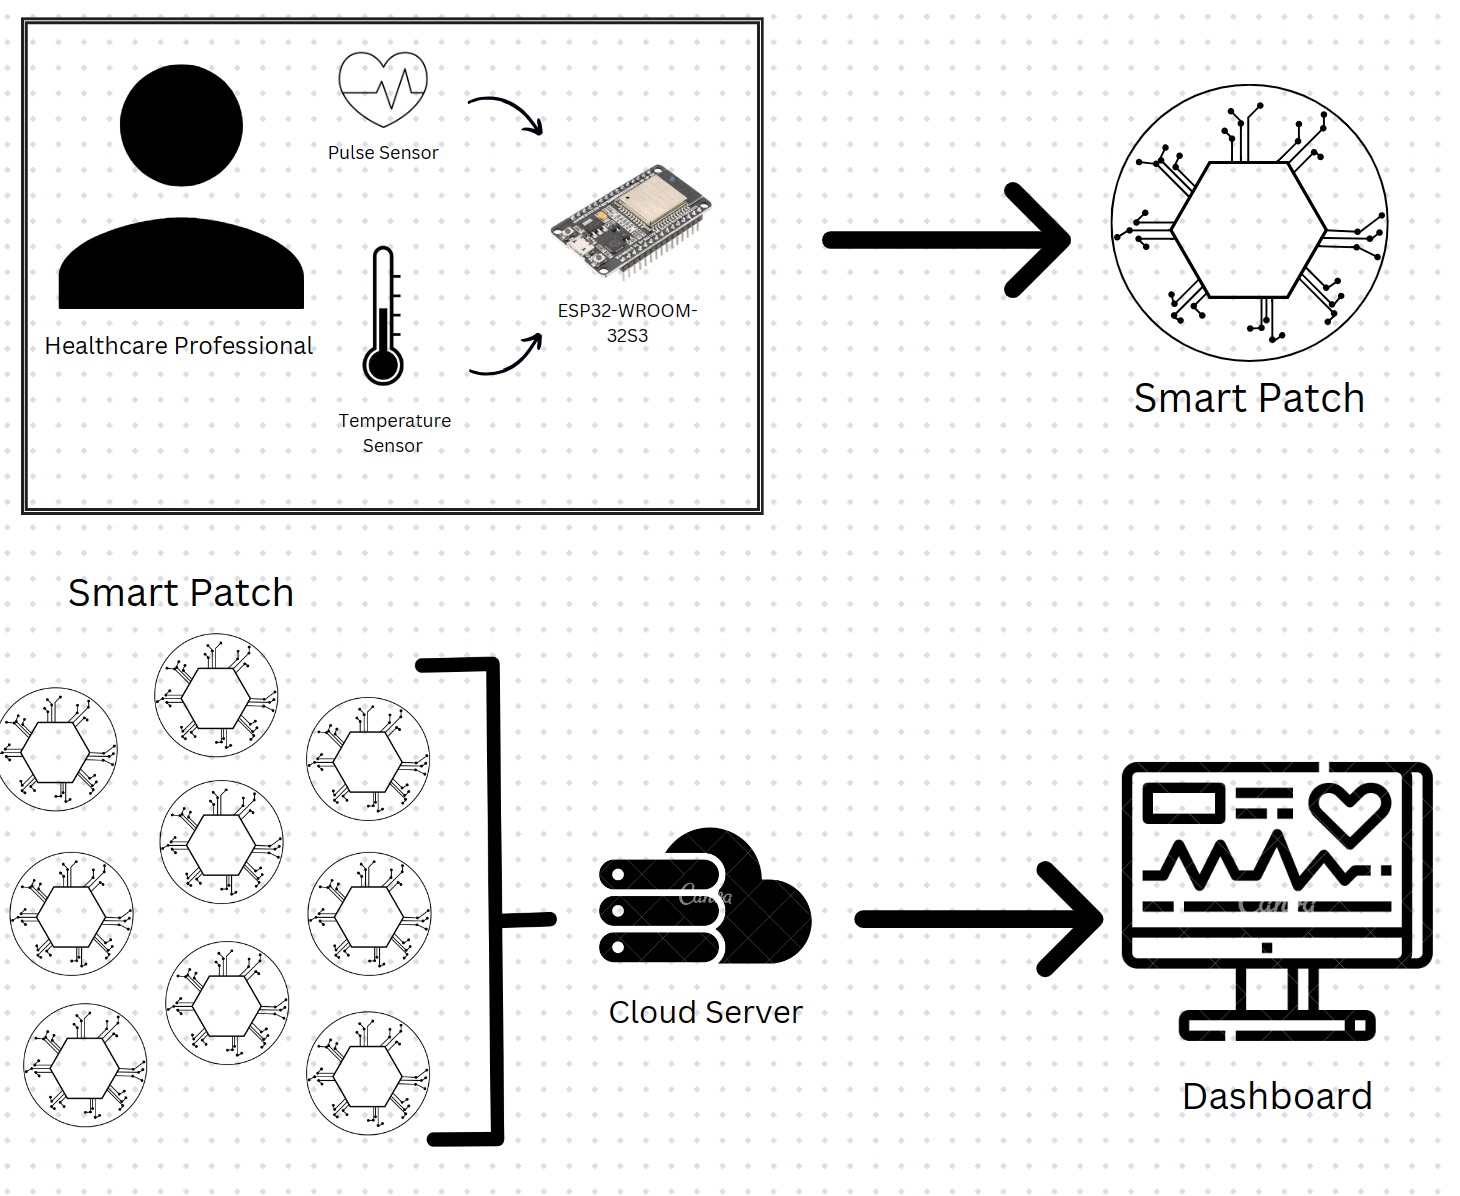
\includegraphics[width=0.9\linewidth]{images/sys-desc.png}
    \caption{VitalMonitor: High-level working diagram}
    \label{fig:sys-desc}
\end{figure}

\subsection{Smart Patch}
The Smart Patch is a non-intrusive wearable IoT device which will be designed to monitor the health and well-being of healthcare professionals in high-stress environments. This innovative IoT device aims to address the limitations of existing wearable technologies, particularly the restrictions on wearing smartwatches in healthcare settings. \\ 

 \noindent While stress and fatigue are complex and multifaceted, heart rate and body temperature serve as surrogate markers that can be effectively measured in real-time. The integration of these parameters into the Smart Patch enables continuous monitoring, offering valuable insights into HCPs’ health and well-being. By focusing on these indicators, the Smart Patch aims to provide actionable data that empowers healthcare institutions to proactively address stress and fatigue, ultimately enhancing the overall quality of care in high-stress environments.
 
 \subsubsection{Device Placement}
The placement of the Smart Patch is crucial to ensure reliable vital sign measurements while minimizing interference with healthcare professionals' tasks. Research in clinical physiology suggests that the ear lobe is an ideal site for accurate and consistent heart rate measurement due to its rich vascular supply and proximity to the surface, which makes it less susceptible to external noise interference and movement artifacts . Additionally, the area behind the ear is well-suited for measuring body temperature, as this region is less exposed to ambient temperature variations than other body surfaces, providing a more accurate reading of core temperature.\\

\noindent Moreover, the ear region provides an advantageous, non-intrusive position where the device is unlikely to interfere with daily tasks. This ensures the comfort and continuous monitoring of HCPs. Figure \ref{fig:device-placement} illustrates the optimal placement of the Smart Patch, highlighting the exact positions on the ear lobe (for heart rate measurement) and behind the ear (for temperature sensing) in red.\\

\noindent By positioning the Smart Patch in these locations, the system can reliably collect data while ensuring that healthcare professionals can work without distraction or discomfort.

 \begin{figure}[h!]
     \centering
     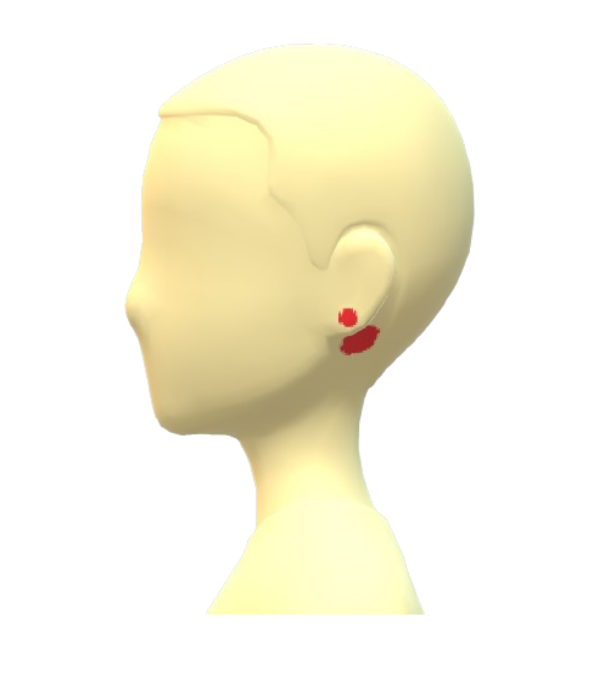
\includegraphics[width=0.3\linewidth]{images/device-placement.png}
     \caption{Device Placement}
     \label{fig:device-placement}
 \end{figure}

\subsection{Dashboard}
 To facilitate real-time monitoring, a web dashboard will be made where the institutions can track the vitals of all the HCPs working at that time using the data being collected by smart patch in real-time. It will present options to get alerts when an HCP’s vital signs go beyond the threshold. Overall,  the dashboard serves as a central hub for visualizing and interpreting the data collected by the smart patch, facilitating informed decision-making and proactive measures to support the health and well-being of HCPs in high-stress environments. \\ \\

\noindent Agile methodology of the Software Development Lifecycle (SDLC) (refer to \textbf{Appendix \ref{app:agile}}) will be used for creating both the Smart Patch and the dashboard.
  
\section{Requirements of the system}
 Both the Smart Patch and the Dashboard boast a set of functional and non-functional requirements meticulously designed to ensure seamless real-time monitoring by healthcare professionals (HCPs). These are categorized as follows: 

  \begin{itemize}
        \item \textbf{User Stories} \\ 
        User stories capture the requirements from the user's perspective, providing insights into their needs. The stories are grouped by user roles. These user stories, along with their priorities, are presented in Table~\ref{tab:longtable}.
        
        \item \textbf{Functional Features} \\
    Functional features represent the capabilities and behaviours of a system that directly contribute to its primary purpose and functionality. These features are concerned with what the system does and how well it performs its intended tasks. 

        \item \textbf{Non-Functional Features} \\
    Non-functional features, on the other hand, are characteristics of a system that do not directly relate to its specific functionalities but rather focus on how well the system performs its functions. 
    
    \end{itemize}
 
 Additionally, they are prioritized using the MoSCoW prioritization framework into Must-Have, Should-Have, Could-Have, and Won’t-Have categories, as illustrated in the Tables \ref{table:functional-sp-db}-\ref{table:non-functional-sp-db}. Key to priority framework is given in Table \ref{tab:key-to-features}.
 

 \begin{table}[h!]
        \centering
        \begin{tabularx}{\textwidth}{|p{3cm}|X|}
            \hline
             \textbf{Category} 
             & \textbf{Description} \\ \hline

             \textbf{Must-Have} 
             & This category consists of features that are “must” for the system. They represent non-negotiable needs for the system.  
             \\ \hline

             \textbf{Should-Have} 
             & 	They are essential for the system, but they are not vital. If left out, the system still functions. However, the features  may add significant value. 
             \\ \hline

             \textbf{Could-Have} 
             & These features are not necessary to the core function of the system. 
             \\ \hline

             \textbf{Won't-Have} 
             & This category contains features which will not be included in a specific release, time frame or prioritised in the future. Their absence is not detrimental to the functionality of the final product.
             \\ \hline 
        \end{tabularx}
        \caption{Key to features}
        \label{tab:key-to-features}
    \end{table} 


    
\clearpage
\subsection{User Stories}
\begin{table}[h]
    \centering
    \begin{tabularx}{\textwidth}{|c|X|c|}
        \hline
        \textbf{User Role} & \textbf{Story} & \textbf{Priority} \\ 
        \hline

        Admin & I want to register my organization. & Must Have \\ 
        \hline
        Admin & I want to log in to the dashboard. & Must Have \\
        \hline
        Admin & I want to add new users. & Must Have \\
        \hline
        Admin & I want to add new devices. & Must Have \\
        \hline
        Admin & I want to manage user-device assignments. & Should Have \\
        \hline
        Admin & I want to monitor vital signs in real-time. & Must Have \\
        \hline
        Admin & I want to securely log out. & Should Have \\
        \hline
        Admin & I want to view a summary of users and devices. & Could Have \\ 
        \hline
        User & I want to wear the device comfortably on my ear. & Won't Have \\
        \hline
        User & I want to easily activate the Smart Patch by pressing a button. & Should Have \\
        \hline
        User & I want to press the button again to stop sending data. & Should Have \\
        \hline
        User & I want the device to continuously measure my heart rate and body temperature while activated. & Must Have \\
        \hline

    \end{tabularx}
    \caption{User Stories for VitalMonitor}
    \label{tab:longtable}
\end{table}


\newpage
\subsection{Functional Requirements (Features)}
\begin{table}[h]
    \centering
    \begin{tabularx}{\textwidth}{|p{3cm}|X|p{2cm}|}
        \hline
        \textbf{Feature}
        & \textbf{Description}
        & \textbf{MoSCoW Priority} \\ \hline
        
        \multicolumn{3}{|l|}{\textbf{Smart Patch Features}} \\ \hline

        Real-time Monitoring
        & Continuously monitors vital signs (HRV and body temperature) in real-time, providing instant feedback on the wearer's physiological status.
        & Must-Have \\ \hline

        Heart Beat Rate Monitoring
        & Monitors heart beat rate of the wearer in real-time.
        & Must-Have \\ \hline

        Body Temperature Monitoring
        & Monitors body temperature of the wearer in real-time.
        & Must-Have \\ \hline

        Wireless Connectivity
        & Equipped with wireless capabilities to securely transmit data to a cloud platform, enabling remote access for healthcare institutions.
        & Must-Have \\ \hline

        \multicolumn{3}{|l|}{\textbf{Dashboard Features}} \\ \hline

        Real-time Monitoring
        & Displays real-time heart rate and body temperature data of HCPs, allowing institutions to track vital signs continuously.
        & Must-Have \\ \hline

        Alerts and Threshold
        & Enables institutions to set and receive alerts when an HCP's vital signs surpass predefined thresholds, facilitating timely intervention in case of abnormal patterns.
        & Must-Have \\ \hline

        Multiple HCP Tracking
        & Supports simultaneous monitoring of multiple HCPs, providing a comprehensive overview of the health status of all professionals working at a given time.
        & Should-Have \\ \hline

        User Authentication
        & Implements secure user authentication to ensure authorized access, maintaining the confidentiality and integrity of healthcare data.
        & Could-Have \\ \hline

        Customizable User Permissions
        & Provides customizable user permissions, allowing institutions to control access levels for different roles, ensuring data privacy and security compliance.
        & Could-Have \\ \hline
    \end{tabularx}
    \caption{Functional Features of the Smart Patch and Dashboard}
    \label{table:functional-sp-db}
\end{table}


\newpage
\subsection{Non-functional Requirements (Features)}
\begin{table}[h!]
    \centering
    \begin{tabularx}{\textwidth}{|p{3cm}|X|p{2cm}|}
        \hline
        \textbf{Feature}
        & \textbf{Description}
        & \textbf{MoSCoW Priority} \\ \hline
        
        \multicolumn{3}{|l|}{\textbf{Smart Patch Non-Functional Features}} \\ \hline

        Non-Intrusiveness
        & Designed to be comfortable for prolonged wear, lightweight, unobtrusive, and adhering to safety and hygiene standards. Placed on the body where least intrusive for healthcare professionals.
        & Must-Have \\ \hline

        Device Portability
        & Designed to be easily portable, allowing healthcare professionals to move freely and perform their duties without hindrance.
        & Must-Have \\ \hline

        Regulatory Compliance
        & Adheres to relevant healthcare and IoT regulatory standards to ensure the device's safety, effectiveness, and compliance with legal requirements.
        & Must-Have \\ \hline

        Long Battery Life
        & Designed with a long-lasting battery to minimize the need for frequent recharging, ensuring continuous monitoring during extended shifts.
        & Should-Have \\ \hline

        Durability
        & Constructed with durable materials to withstand daily wear and tear in a healthcare environment, ensuring the device's longevity and reliability.
        & Should-Have \\ \hline

        Compatibility
        & Ensures compatibility with various body types and sizes, accommodating diverse healthcare professionals with different preferences and needs.
        & Should-Have \\ \hline

        \multicolumn{3}{|l|}{\textbf{Dashboard Non-Functional Features}} \\ \hline

        User-Friendly Interface
        & Designs an intuitive and user-friendly dashboard interface, enhancing the overall experience for healthcare professionals and administrators interacting with the monitoring system.
        & Must-Have \\ \hline

        Performance Optimization
        & Optimizes the dashboard's performance to handle real-time data efficiently, ensuring a smooth and responsive user experience even during periods of high data traffic.
        & Should-Have \\ \hline

        Scalability
        & Designs the dashboard to be scalable, accommodating potential future expansions in the number of monitored healthcare professionals without compromising performance or user experience.
        & Should-Have \\ \hline

        Security and Compliance
        & Ensures data security by implementing robust measures to protect sensitive healthcare information, complying with relevant regulations and industry standards.
        & Should-Have \\ \hline

    \end{tabularx}
    \caption{Non-Functional Features of Smart Patch and Dashboard}
    \label{table:non-functional-sp-db}
\end{table}

\newpage
\section{Risk Analysis}
 This section lists down all the potential risks that this project might face. The risk register provided in Figure \ref{fig:rr} is continuously updated throughout the project timeline as per the key to risk rating provided in Figure in \ref{fig:ktrr}.

\vspace{5.5cm}
\noindent\textbf{Key to Risk Rating:}
\begin{figure}[h!]
    \centering
    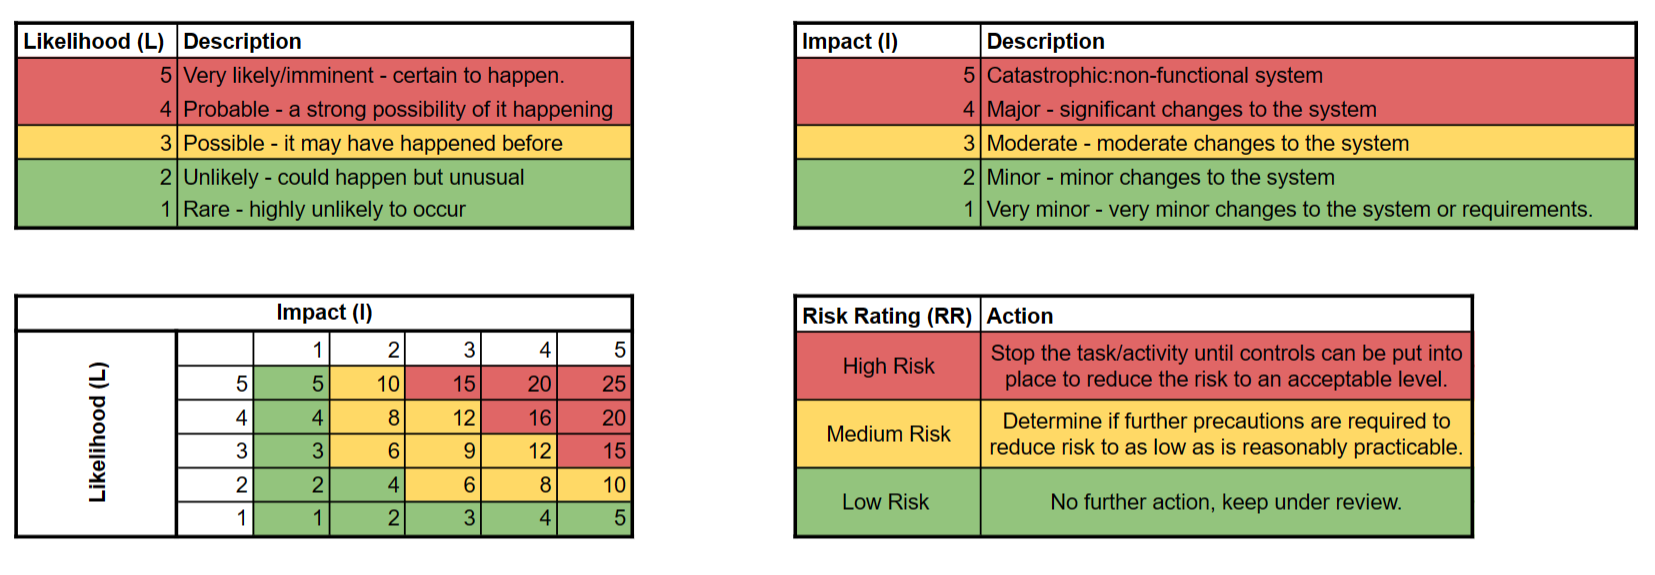
\includegraphics[width=1\linewidth]{images/ktrr.png}
    \caption{Key to Risk Rating}
    \label{fig:ktrr}
\end{figure}

\begin{figure}
    \centering
    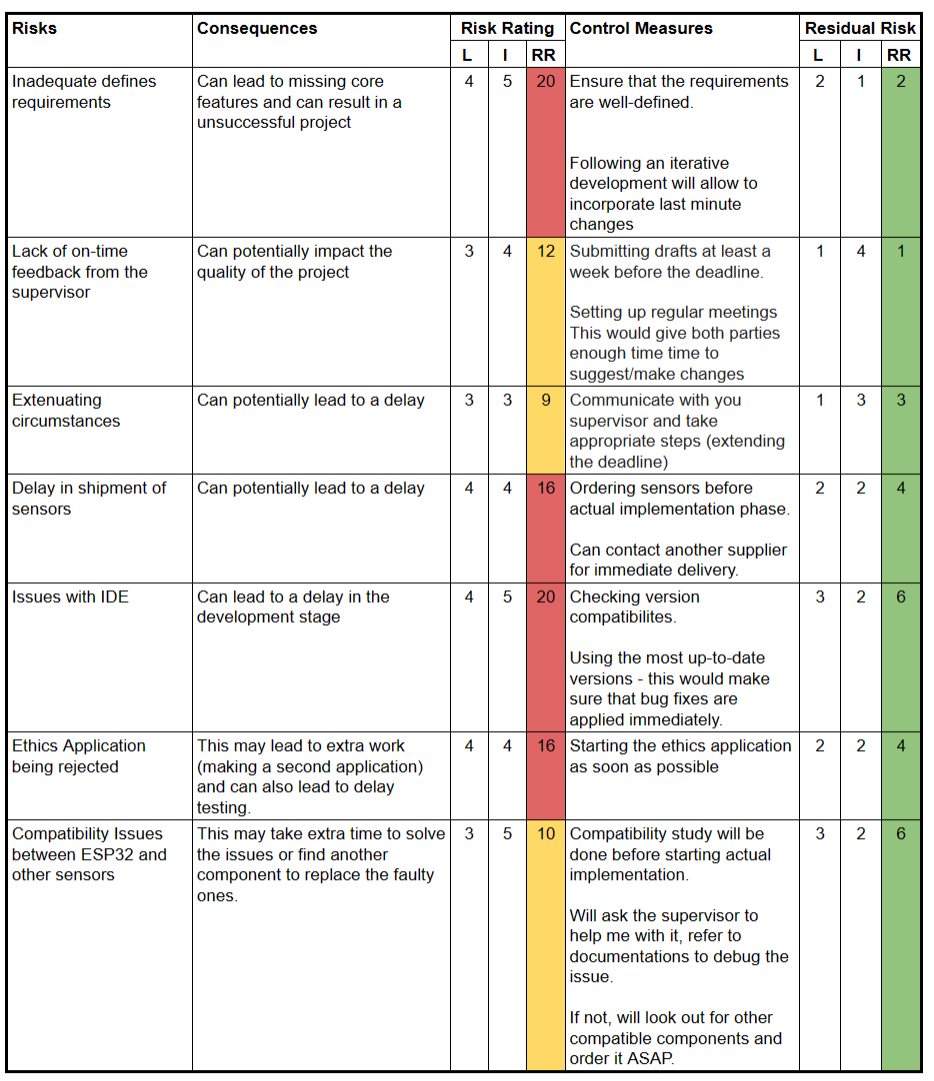
\includegraphics[width=1\linewidth]{images/rr.png}
    \caption{Risk Register}
    \label{fig:rr}
\end{figure}

\newpage
\section{Evaluation}
To ensure the robustness, reliability, and effectiveness of the Smart Patch and the dashboard, a comprehensive testing and quality assurance process will be implemented throughout the implementation and testing stage of the project:
\begin{itemize}
    \item \textbf{Unit tests:} Conducted to validate the correctness of individual components and the functionality of the Smart Patch and dashboard.
    \item \textbf{Integration testing:} Conducted to verify the seamless integration of components and modules within the Smart Patch and the dashboard.
    \item \textbf{System testing:} Conducted to assess the overall functionality and the performance of the integrated Smart Patch and the dashboard.
    \item \textbf{Acceptance Testing:} Covering all user stories to ensure that the system meets user requirements.
    \item \textbf{Manual testing:} For features that cannot be adequately tested using the above tests.
\end{itemize} 
A systematic evaluation of legal and ethical considerations will also take place:
\begin{enumerate}
    \item \textbf{Legal considerations:} Medical Regulations outlined by MHRA and GDPR guidelines will be followed (see \textbf{Appendix \ref{app:legal}}).
    \item \textbf{Ethical considerations:} Guidelines provided by the University of Sheffield will be followed, and an ethics application will be made if the project starts to use real human health data other than the developers' data (see \textbf{Appendix \ref{app:ethical}}).
\end{enumerate}



\newpage

\chapter{Technology Stack}
This chapter will cover on technology stack needed to build the smart patch and the dashboard. It will provide an overview of what might be needed, possible technologies to choose from and choosing the most suitable ones for the development of the system.

\section{Firmware for Smart Patch}

\subsection{Computing Units - Microcontrollers (MCU)}
A microcontroller (MCU) is a compact, self-contained computer integrated on a single chip, designed for embedded applications with lightweight processing needs \cite{ref22}. MCUs are known for their small size, low power consumption, and cost-effectiveness. MCUs require a hands-on approach, involving configuration for both hardware (attachment of components, sensors, wires, etc.) and software (burning firmware, incorporating libraries, installing drivers, etc.). MCUs lack a conventional operating system and utilize firmware, a special code burned onto the device to execute specific functions and ensure proper hardware functionality. While they cannot serve as personal computers, some advanced MCUs offer features like networking, making them appealing for projects with specific requirements. \\

\begin{figure}[h!]
    \centering
    \begin{subfigure}{0.45\linewidth} % Adjust the width as needed
        \centering
        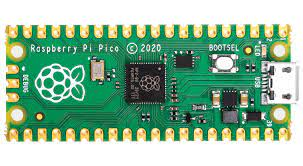
\includegraphics[width=\linewidth]{images/pico.jpg}
        \caption{Raspberry Pi Pico \cite{ref23}}
        \label{fig:pico}
    \end{subfigure}
    \hfill % This command adds space between subfigures
    \begin{subfigure}{0.45\linewidth} % Adjust the width as needed
        \centering
        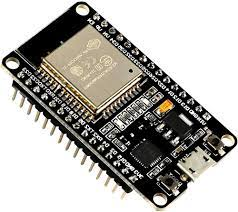
\includegraphics[width=\linewidth]{images/esp32(1).jpg}
        \caption{ESP32 \cite{ref24}}
        \label{fig:esp32}
    \end{subfigure}
    \caption{Comparison of Microcontrollers}
    \label{fig:comparison}
\end{figure}

\noindent There are multiple MCUs available in the market but the most popular ones are Raspberry Pi Pico and ESP32-WROOM-32S3-Mini-1. A comparative study between the two is provided in Table \ref{table:microcontrollers} to help in choosing the ideal MCU. \\

\begin{table}[h!]
\centering
\begin{tabularx}{\textwidth}{|X|X|X|}
\hline
\textbf{Feature} & \textbf{Raspberry Pi Pico} & \textbf{ESP32-WROOM-32S3-Mini-1} \\ \hline
Manufacture & Raspberry Pi Foundation & Espressif Systems \\ \hline
Architecture & ARM Cortex-M0+ & Xtensa LX6 \\ \hline
Processor Clock Speed & Up to 133 MHz & Up to 240 MHz \\ \hline
Wireless Connectivity & None & Wi-Fi, Bluetooth (BLE) \\ \hline
Memory & 2MB Flash (No built-in RAM) & 2MB Flash \\ \hline
GPIO Pins & 26 & Approximately 38 \\ \hline
Development Environment & MicroPython, C/C++ with Pico SDK & Arduino IDE, PlatformIO, Espressif IDF \\ \hline
\end{tabularx}
\caption{Comparative study between Raspberry Pi Pico and ESP32-WROOM-32S3-Mini-1}
\label{table:microcontrollers}
\end{table} 

\noindent Comparing the two, ESP32-WROOM-32S3-Mini-1 comes out as ideal for the Smart Patch because of its in-built wireless connectivity. It is important to have such connectivity to provide portability of the device so that wearer can wear it all day and still can go around the campus.

\noindent To power the microcontroller, we'll either provide direct power through the C-pin or utilize a LiPo battery for portability and extended use.

\subsection{Sensors}
MCUs typically come equipped with general-purpose I/O pins (GPIO), allowing users to connect various external peripherals to the computer. Examples of common input devices include sensor modules, microphones, and cameras, while output devices encompass LEDs, speakers, displays, and more. Users can program these individual pins to receive data. 

\subsubsection{Heart Rate Sensors}
To calculate HRV, heart rate sensors have to be used and connected with the MCU. Two sensors which are used abundantly in the industry, especially healthcare are ECG Sensors and Pimoroni Pulse Sensor. A comparative study is provided in Table \ref{table:heart-rate-sensor} to help in determining the ideal sensor. 

\begin{table}[p]
\centering
\begin{tabularx}{\textwidth}{|X|X|X|}
\hline
\textbf{Features} & \textbf{ECG Sensor} & \textbf{Pimoroni Pulse Sensor} \\ \hline
\textbf{Working Principle} &
ECG Sensor measures the heart's electrical activity over time \cite{ref25}. It detects the heartbeat rhythm regularly to keep a check on the health of your heart \cite{ref26}. &
Pimoroni Pulse Sensor uses a technique called photoplethysmography (PPG) to detect the change in the colour of your skin with each beat of your heart when the sensor is pressed against your fingertip \cite{ref27}. \\ \hline
\textbf{Use Cases} & 
It can detect Arrhythmias like Atrial fibrillation and can also warn you about heart attack using strokes and movements around the heart. & 
It can be used by students, artists, athletes, makers, and game \& mobile developers who want to easily incorporate live heart-rate data into their projects. \\ \hline
\textbf{Compatibility} &
Works with most smartwatches. &
Works with Arduino, micro:bit, littleBits, and most maker platforms. \\ \hline
\textbf{Intrusivity} &
Non-invasive requires skin contact. &
Less intrusive, fingertip contact. \\ \hline
\textbf{Additional Features} & 
Some devices can export an ECG graph of your heart rate, which can be a huge help when talking to your doctor. &
The Pulse Sensor has 3 holes around the outside edge which make it easy to sew it into almost anything. \\ \hline
\textbf{Image} & 
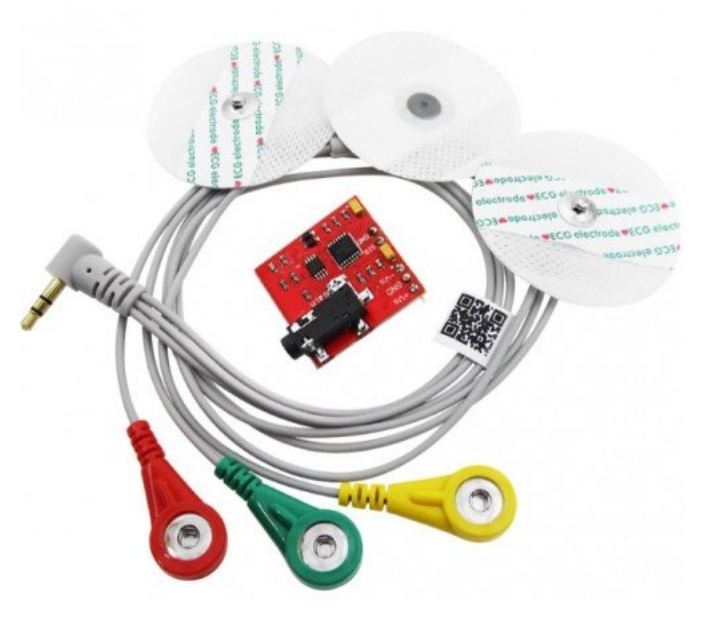
\includegraphics[width=\linewidth]{images/ecg.png}
& 
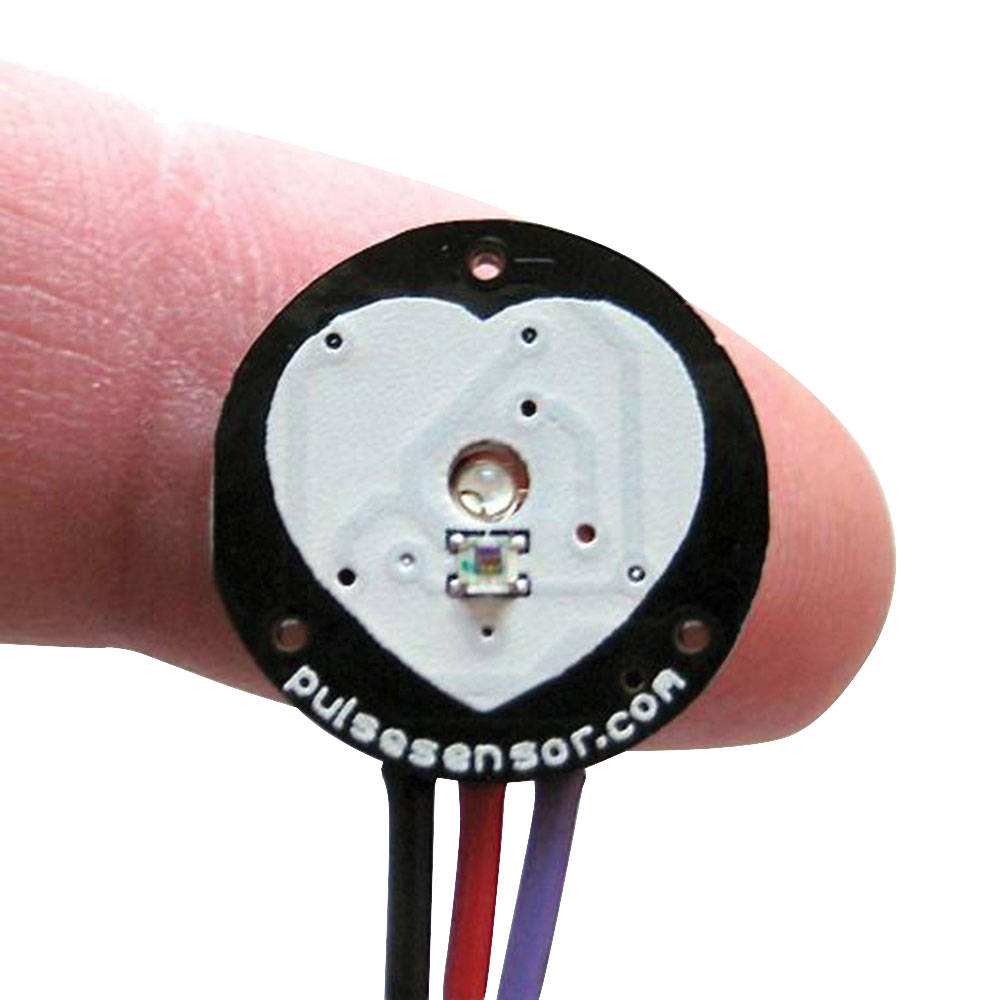
\includegraphics[width=\linewidth]{images/s75-0818p01wj.jpg}
\\ \hline

\end{tabularx}
\caption{Comparative Study between ECG Sensor and Pimoroni Pulse Sensor}
\label{table:heart-rate-sensor}
\end{table}

One of the main features of the Smart Patch is non-intrusivity. While both the sensors are efficient and used widely, Pulse Sensor comes out as a perfect choice for Smart Patch because not only it is less intrusive but also it works well with ESP32 (Arduino).

\subsubsection{Body Temperature Sensor}
To calculate body temperature, thermometers are used normally in healthcare. But thermometers are not digital devices and therefore can’t be connected to the smart patch. Other sensors which are widely used for sensing temperature are thermistors, LM-35 sensors and DS18B20. Thermistors are more temperature-sensitive resistors and not sensors and require a readout circuit, which makes it harder to integrate them seamlessly into Smart Patch.  \\

\begin{figure}[!h]
    \centering
    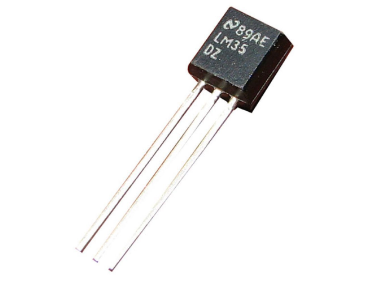
\includegraphics[width=0.25\linewidth]{images/lm-35-image.png}
    \caption{LM-35 Sensor \cite{ref28}}
    \label{fig:lm-35-sensor}
\end{figure}

\noindent On the other hand, the LM-35 Sensor is a precision IC temperature sensor. It provides a linear voltage vs temperature characteristic making it easier to figure out the temperature. It can operate over a temperature range of \(−55 ^\circ C\) to \(150 ^\circ C\) and has an accuracy of \(\pm1\) degree Celsius. Additionally, its analog output allows for simple integration with the analog-to-digital converter of the microcontroller used in the Smart Patch. \\

\begin{figure}[h!]
    \centering
    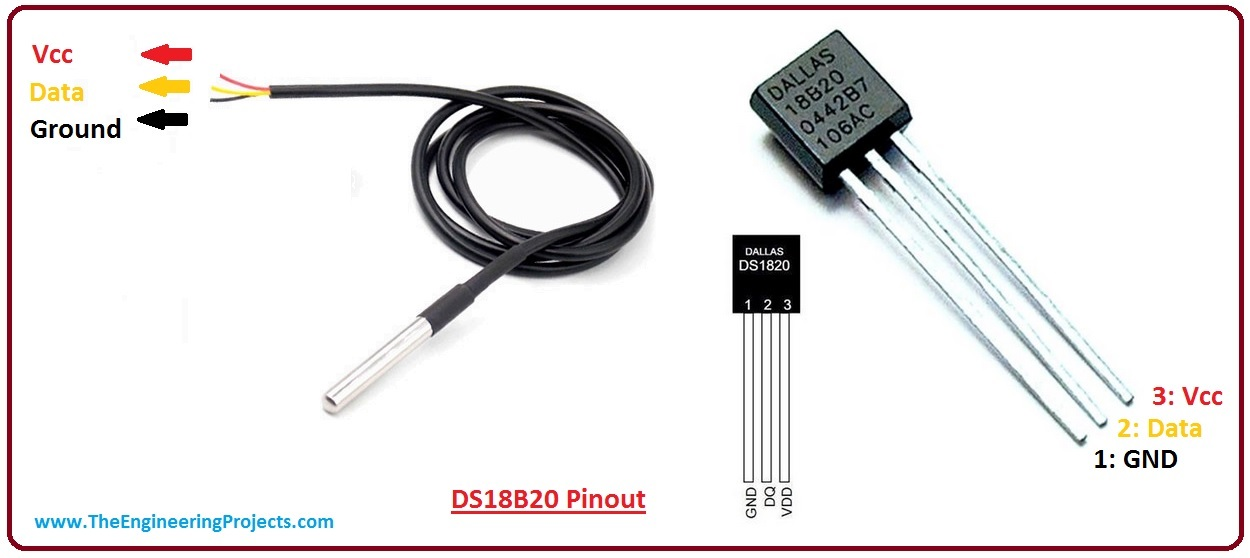
\includegraphics[width=0.75\linewidth]{images/ds18b20.png}
    \caption{DS18B20 Sensor \cite{51}}
    \label{fig:ds18b20}
\end{figure}

\noindent Lastly, the DS18B20 sensor is a digital temperature sensor with a unique 1-wire interface that allows it to communicate efficiently with the Smart Patch's processing unit. It operates in the range of \(-55^\circ C\) to \(125^\circ C\) and boasts an accuracy of \(\pm0.5^\circ C\) over the range of \(-10^\circ C\) to \(85^\circ C\). Additionally, the DS18B20 supports multiple devices on the same bus, enabling the monitoring of multiple sensors using only one microcontroller input. Its digital output makes it immune to noise and interference, providing reliable measurements. \\

\noindent Both the LM-35 and DS18B20 have notable features. The project will test both sensors and retain the one that demonstrates superior accuracy and reliability.

\subsection{Connectivity Technology}
Connective Technology is nothing but a network of connected “smart” devices that communicate seamlessly over the internet. Wi-Fi, Bluetooth and LoRaWAN are the most used networks associated with IoT. Table \ref{table:connective-technology} provides a comparative study between the three to help in choosing the most suitable technology for the project.\\
\begin{table}[h]
    \centering
    \begin{tabularx}{\textwidth}{|X|X|X|X|}
        \hline
        \textbf{Features} & \textbf{Wi-Fi} & \textbf{Bluetooth} & \textbf{LoRaWAN} \\ \hline
        \textbf{Scalability} & Limited for massive IoT. & Mesh supports large networks. & Scales well for wide area. \\ \hline
        \textbf{Power Efficiency} &  High power consumption.& Low Energy, efficient. & Low power usage. \\ \hline
        \textbf{Range and Coverage} & Short to medium range.&Moderate, indoor range.&Long-range, wide coverage. \\ \hline
        \textbf{Data Rate} & High-speed data transfer & Moderate data rates & Low data rates \\ \hline
        \textbf{Cost and Infrastructure} & Existing infrastructure may be costly. & Cost-effective, integrated widely. & Low infrastructure cost\\ \hline
        \textbf{Security} & Robust encryption, authentication & Secure with enhancements& Implement AES encryption \\ \hline
    \end{tabularx}
    \caption{Comparative Study between Connective Technologies}
    \label{table:connective-technology}
\end{table}

\begin{figure}
        \centering
        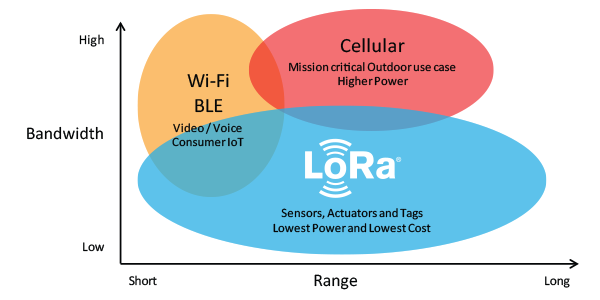
\includegraphics[width=\linewidth]{images/connective-technology.png}
        \caption{Connective Technologies compared against Bandwidth and Range \cite{ref29}}
        \label{fig:connective-technology}
    \end{figure}

From the comparison in Table \ref{table:connective-technology} and Figure \ref{fig:connective-technology}, LoRaWAN stands out as a clear and most efficient choice for Smart Patch. But the only disadvantage is that this network is not usually found in healthcare institutions compared to Wi-Fi which is available in nearly every healthcare institution. This advantage of Wi-Fi makes it easier to integrate Smart Patch with existing resources of institution thereby saving extra cost and other resources. Hence, Smart Patch will use Wi-Fi as its connective technology.

\newpage
\section{Software for Smart Patch}
\subsection{Programming Environment}
Arduino IDE, Espressif IDF (IoT Development Framework), and PlatformIO are three different programming environments used for developing software for microcontrollers and embedded systems. Each has its own strengths, weaknesses, and use cases.

\begin{table}[h]
    \centering
    \begin{tabularx}{\textwidth}{|X|X|X|X|}
        \hline
            
         & \textbf{Arduino IDE} 
         & \textbf{Espressif IDF} 
         & \textbf{PlatformIO} \\ \hline

         \textbf{Purpose} 
         & Beginner-friendly prototyping 
         & Advanced ESP32/ESP8266 development
         & Cross-platform IoT development \\ \hline

         \textbf{Language Support}
         & C/C++ with simplified syntax
         & Full C/C++ language support
         & Supports multiple languages \\ \hline

         \textbf{Hardware Compatibility}
         & Extensive hardware compatibility
         & Specifically for ESP32/ESP8266 
         & Broad hardware support \\ \hline

         \textbf{Integration}
         & Integrated Development Environment
         & Integrated toolchain for ESP 
         & Integrated platform and library manager \\ \hline
    
    \end{tabularx}
    \caption{Comparative Study between Programming Environments}
    \label{table:programming-environment}
\end{table}

For the project, Arduino IDE emerges as the preferred choice after comparing the three environments (as outlined in Table \ref{table:programming-environment}). Its beginner-friendly nature suits the project's prototyping needs, and it offers extensive hardware compatibility. Additionally, Arduino IDE's simplified syntax aligns well with the project's requirements.

\subsection{Programming Languages}
ESP32 is compatible with 2 programming languages - Arduino C++ and MicroPython. Both of these languages are popular and used widely to program the firmware. The table \ref{table:programming-language} provides features of each of these languages.

\begin{table}[h]
    \centering
    \begin{tabularx}{\textwidth}{|X|X|X|}
        \hline

        \textbf{Features}
         & \textbf{Arduino C++}
         & \textbf{MicroPython} \\ \hline

        \textbf{Use} 
        & Firmware
        & Firmware \\ \hline

        \textbf{Programming Language}
        & Low-level language with simplified syntax.
        & Python optimized for microcontrollers. \\ \hline

        \textbf{Abstraction level}
        & Provides abstraction for hardware complexities.
        & Abstracts hardware with clean Python code. \\ \hline

        \textbf{Ease of Use}
        & Beginner-friendly with a simplified structure.
        & Beginner-friendly, less complex than C/C++. \\ \hline

        \textbf{Memory Usage}
        & Generally efficient memory usage. 
        & May use more memory compared to C/C++. \\ \hline

        \textbf{Application Scope}
        & Ideal for firmware development in embedded systems.
        & Suited for microcontroller programming. \\ \hline

        \textbf{Ecosystem}
        & Rich ecosystem, extensive libraries.
        & Growing ecosystem for microcontrollers. \\ \hline

        \textbf{Concurrency Model}
        & Sequential execution with setup() and loop().
        & Supports concurrency but less efficiently. \\ \hline

        \textbf{Frameworks}
        & Arduino framework for embedded systems.
        & Limited frameworks for microcontrollers. \\ \hline

        \textbf{Resource Efficiency}
        & Generally efficient in resource usage.
        & May consume more resources. \\ \hline
         
    \end{tabularx}
    \caption{Comparative Study between Arduino C++ and MicroPython}
    \label{table:programming-language}
\end{table}

\noindent Both programming languages demonstrate efficiency in their respective ways.  To determine the most suitable choice for the project, a decision matrix is employed (shown in Table \ref{fig:decision-matrix}). Each crucial feature is assessed for both languages, assigning a weighted score to each feature. Both scores and weights are provided in a range of 1 to 5.

% \begin{figure}
%     \centering
%     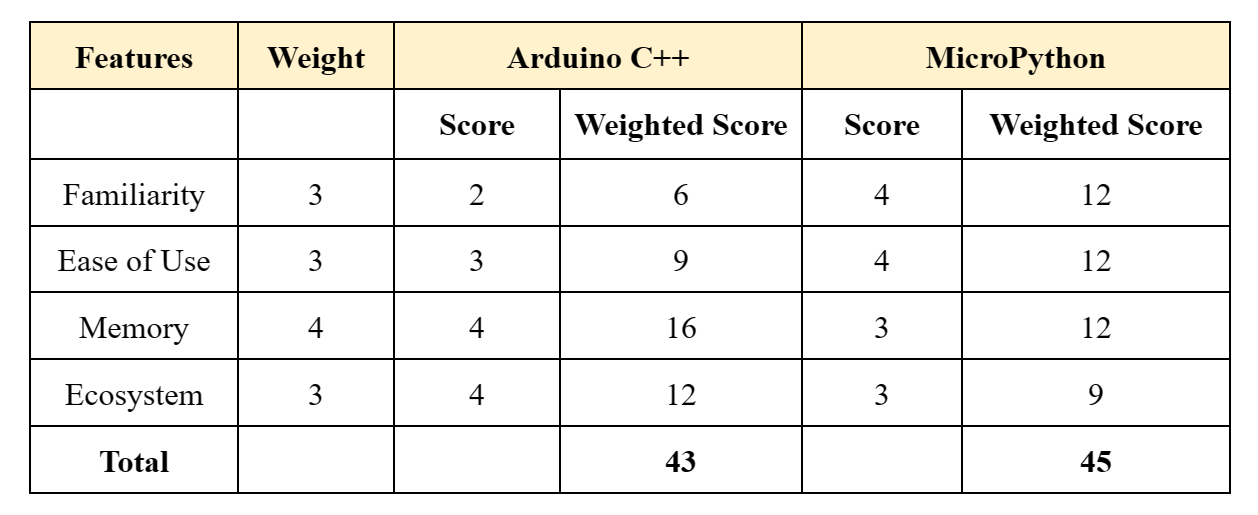
\includegraphics[width=1\linewidth]{images/decision-matrix.png}
%     \caption{Decision Matrix for Programming Languages}
%     \label{tab:decision-matrix}
% \end{figure}

\begin{table}[!h]
\centering
\begin{tabularx}{\textwidth}{|X|X|X|X|X|X|}
    \hline
    \textbf{Features} 
    & \textbf{Weight}
    & \multicolumn{2}{c|}{\textbf{Arduino C++}}
    &  \multicolumn{2}{c|}{\textbf{MicroPython}}  \\ \hline

    &
    & Score 
    & Weighted Score
    & Score 
    & Weighted Score \\ \hline

    Familiarity 
    & 3 
    & 2 
    & 6
    & 3
    & 9 \\ \hline
    
    Ease of Use
    & 3 
    & 3 
    & 9
    & 4 
    & 12 \\ \hline
    
    Memory 
    & 4 
    & 4 
    & 16
    & 3 
    & 12 \\ \hline
    
    Ecosystem 
    & 3 
    & 4 
    & 12
    & 3 
    & 9 \\ \hline
    
    \textbf{Total} 
    & 
    &
    & \textbf{43} 
    &  
    & \textbf{42}  \\ \hline
    
\end{tabularx}
\caption{Decision Matrix for Programming Languages}
\label{fig:decision-matrix}
\end{table}

\noindent Following the completion of the decision matrix, it is determined that Arduino C++ emerges as the more fitting choice of programming language for the project. \\

Alternatively, a variety of IoT solutions are accessible in the market and offered at no cost. These options span from frameworks for creating dashboards to robust cloud platforms specifically designed for IoT applications. (see \textbf{Appendix E})\\

\section{Software for Web Dashboard}
The dashboard would be nothing but a website made using HTML, CSS and Javascript (JS). The programming environment of choice will be Visual Studio Code (VSCode), providing a robust platform for web development. \\

\noindent The Flask framework will be utilized for developing the backend framework of the web dashboard. Flask is a lightweight and flexible micro-framework for Python. It offers simplicity and ease of use, making it suitable for building web applications. \\ \\
Additionally, a mixture of SQLite (for testing) and MySQL (for production) databases will be employed to manage data storage and retrieval efficiently. 
\begin{enumerate}
    \item SQLite offers a lightweight and self-contained database solution, ideal for testing and development environments. Its simplicity and zero-configuration setup streamline the process of data storage and retrieval during development.
    \item MySQL is a robust relational database management system, is well-suited for production environments due to its scalability, performance, and reliability. It provides advanced features for managing large datasets and ensuring data integrity for the web dashboard in a production setting.
\end{enumerate}

\section{Messaging API: Twilio API}
The Twilio API provides a robust platform for integrating messaging capabilities into IoT Devices. With Twilio, developers can send and receive SMS, MMS, and even WhatsApp messages programmatically, enabling real-time communication with users. Twilio API offers versatile messaging channels, global coverage, developer-friendly API, scalability, reliability, and security. This makes it the ideal choice for integrating seamless and efficient communication capabilities into the web dashboard.\\ \\

\noindent Within the project scope, a thorough examination of potential risks has been undertaken, delineating possible difficulties that might emerge throughout the project’s duration. The risk register will be reviewed regularly throughout the project, allowing for the timely incorporation of newly recognised risks and fostering a proactive approach to risk management.  The primary emphasis of this section is on identifying major potential risks and devising strategies to minimise their effects. \textbf{Appendix F} provides the risk register used for the project.


\chapter{Design}

The Design chapter talks about the architectural blueprint of VitalMonitor. This includes an overview of the system's architecture, followed by an in-depth analysis of each component's design and role within the larger ecosystem. From the setting up of the database to the intricate firmware running on each smart patch, the design choices made across VitalMonitor will be explored to elucidate their contributions to the system's overall functionality, reliability, and scalability. This chapter is written in accordance with v8 iteration of the firmware.\\

Additionally, the chapter illustrates the thoughtful considerations behind the chosen architectural patterns, dissects the interactions between system components, and explains the rationale behind the design decisions. This chapter sets the stage for understanding how each element of VitalMonitor contributes to a cohesive and robust system.

\section{System Design}
\subsection{Design Approach}

\noindent The system design of VitalMonitor integrates multiple architectural principles, deviating from traditional approaches to create a tailored solution. It is structured into three primary layers: Presentation, Application, and Data Layer.

\begin{itemize}
    \item \textbf{Presentation Layer:}  The web dashboard serves as the presentation layer, providing a user interface (UI) for users to interact with the system. This layer presents data collected from IoT devices in a visual and understandable format through the dashboard.
    
    \item \textbf{Application Layer:} The middleware component serves as the application layer, handling the business logic of receiving, and distributing data from Smart Patches. It acts as an intermediary between the presentation layer and the data layer, performing tasks such as data aggregation and routing.
    
    \item \textbf{Data Layer:} The Smart Patches represent the data layer, where data is generated and collected from the real world. This raw data from sensors is then processed and transmitted to the middleware for further processing and storage.

    
\end{itemize}
Communication between these layers primarily occurs through APIs, designed following RESTful principles to promote simplicity and flexibility. \\ \\
Moreover, the Smart Patch logic adopts a hybrid architecture:
\begin{itemize}
    \item \textbf{Edge-Computing:} Edge Computing optimizes data processing by executing computations closer to the data source (here the Smart Patch), effectively reducing latency and conserving bandwidth. This strategy facilitates local data processing, eliminating irrelevant information and transmitting only essential insights to the cloud.  Urgent actions, like sending emergency SMS via Twilio API, are executed swiftly at the edge to minimize delays.
    
    \item \textbf{Cloud-Based:} The cloud serves dual purposes: firstly, as a data repository, and secondly, for processing incoming data from devices. Settings originating from the Presentation layer are forwarded to Smart Patches from the cloud.

\end{itemize}

\noindent This design rationale was chosen to:
\begin{enumerate}
\item Enhance flexibility in development and deployment processes.
\item Facilitate continuous integration and delivery practices.
\item Inherently support a distributed data processing model, crucial for IoT environments.
\end{enumerate}

\subsection{Component Roles and Ideology}

\noindent{VitalMonitor operates on a coordinated data flow mechanism, where each component plays a critical role. Each component is designed with a specific role in mind as per the above design choices. This systematic interaction ensures seamless end-to-end data flow, from data capture to user-level presentation. The components are: }

\begin{itemize}
    \item The Dashboard is the user interface through which users interact with the system. It is designed to offer intuitive controls and insightful analytics.

    \item The Smart Patch is a component of VitalMonitor, equipped with sensors and a microcontroller to accurately collect and relay vital health data.

    \item The Middleware acts as the central nervous system, directing the flow of information and ensuring the components of VitalMonitor communicate effectively.
\end{itemize}

\subsection{Data Flow Architecture}
\noindent{Figure \ref{fig:dfd-1} illustrates the interconnectivity and the specific pathways through which data travels within the VitalMonitor system. This diagram provides a visual representation of the sequential and logical flow of data, from the initial collection at the smart patch, through processing by the middleware, to its final storage and presentation in the dashboard. Figure \ref{fig:dfd-2} goes further into how a Smart Patch gets data from sensors and integrates with Twilio API and Adafruit IO. It exemplifies how the design ensures not only the efficient management of data but also its security and integrity as it moves through various system components.}

\begin{figure}[h!]
    \centering
    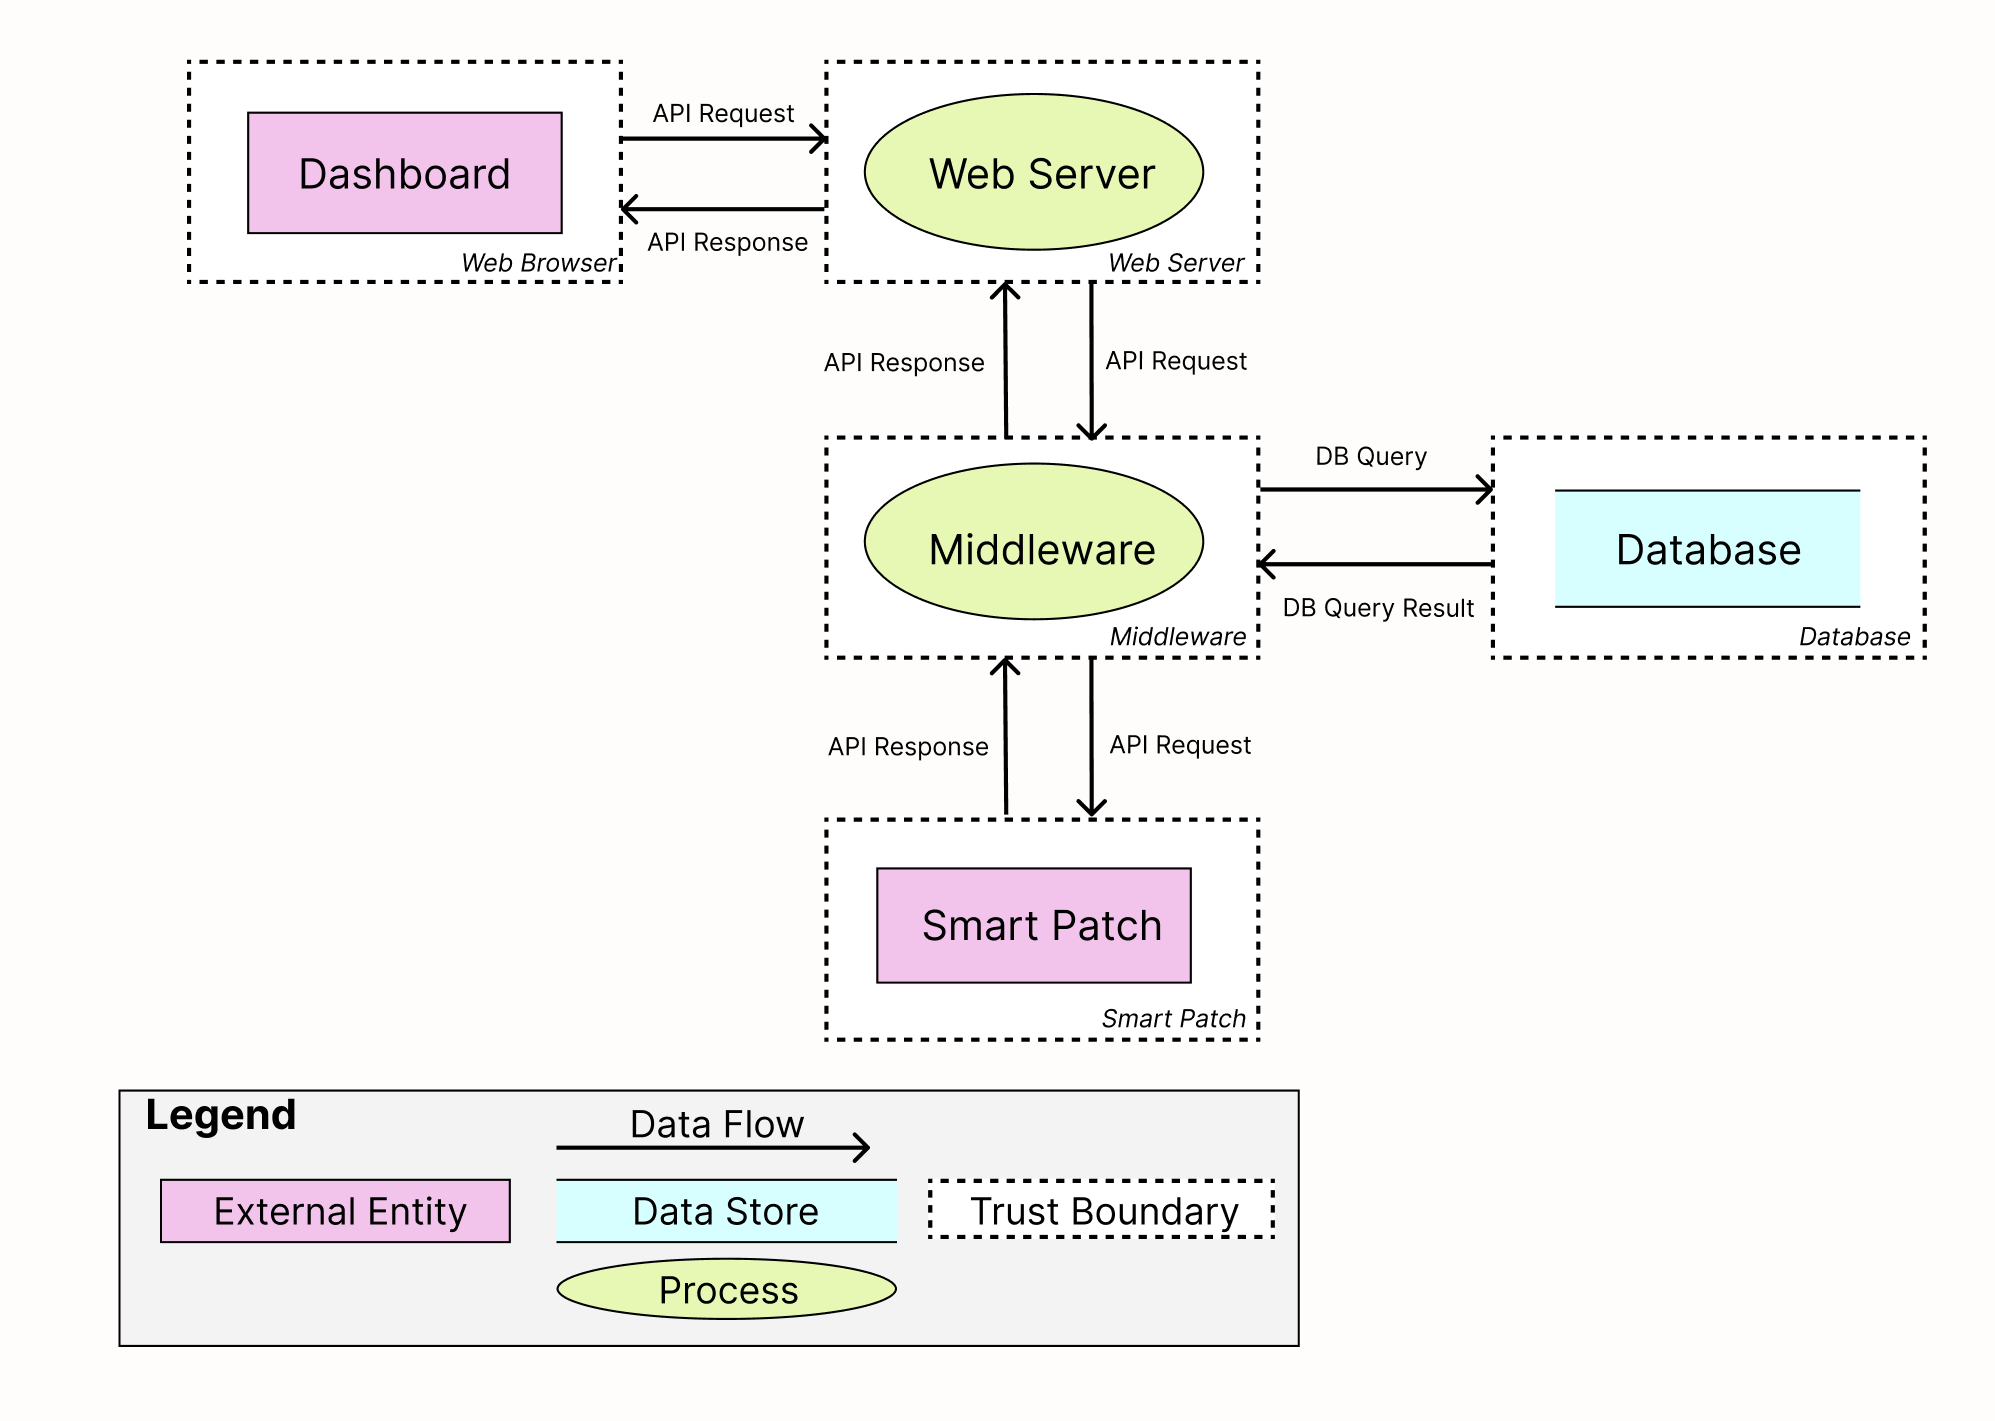
\includegraphics[width=1\linewidth]{images/system-design-data-flow-full.png}
    \caption{Data Flow Diagram 1}
    \label{fig:dfd-1}
\end{figure}

\begin{figure}[h!]
    \centering
    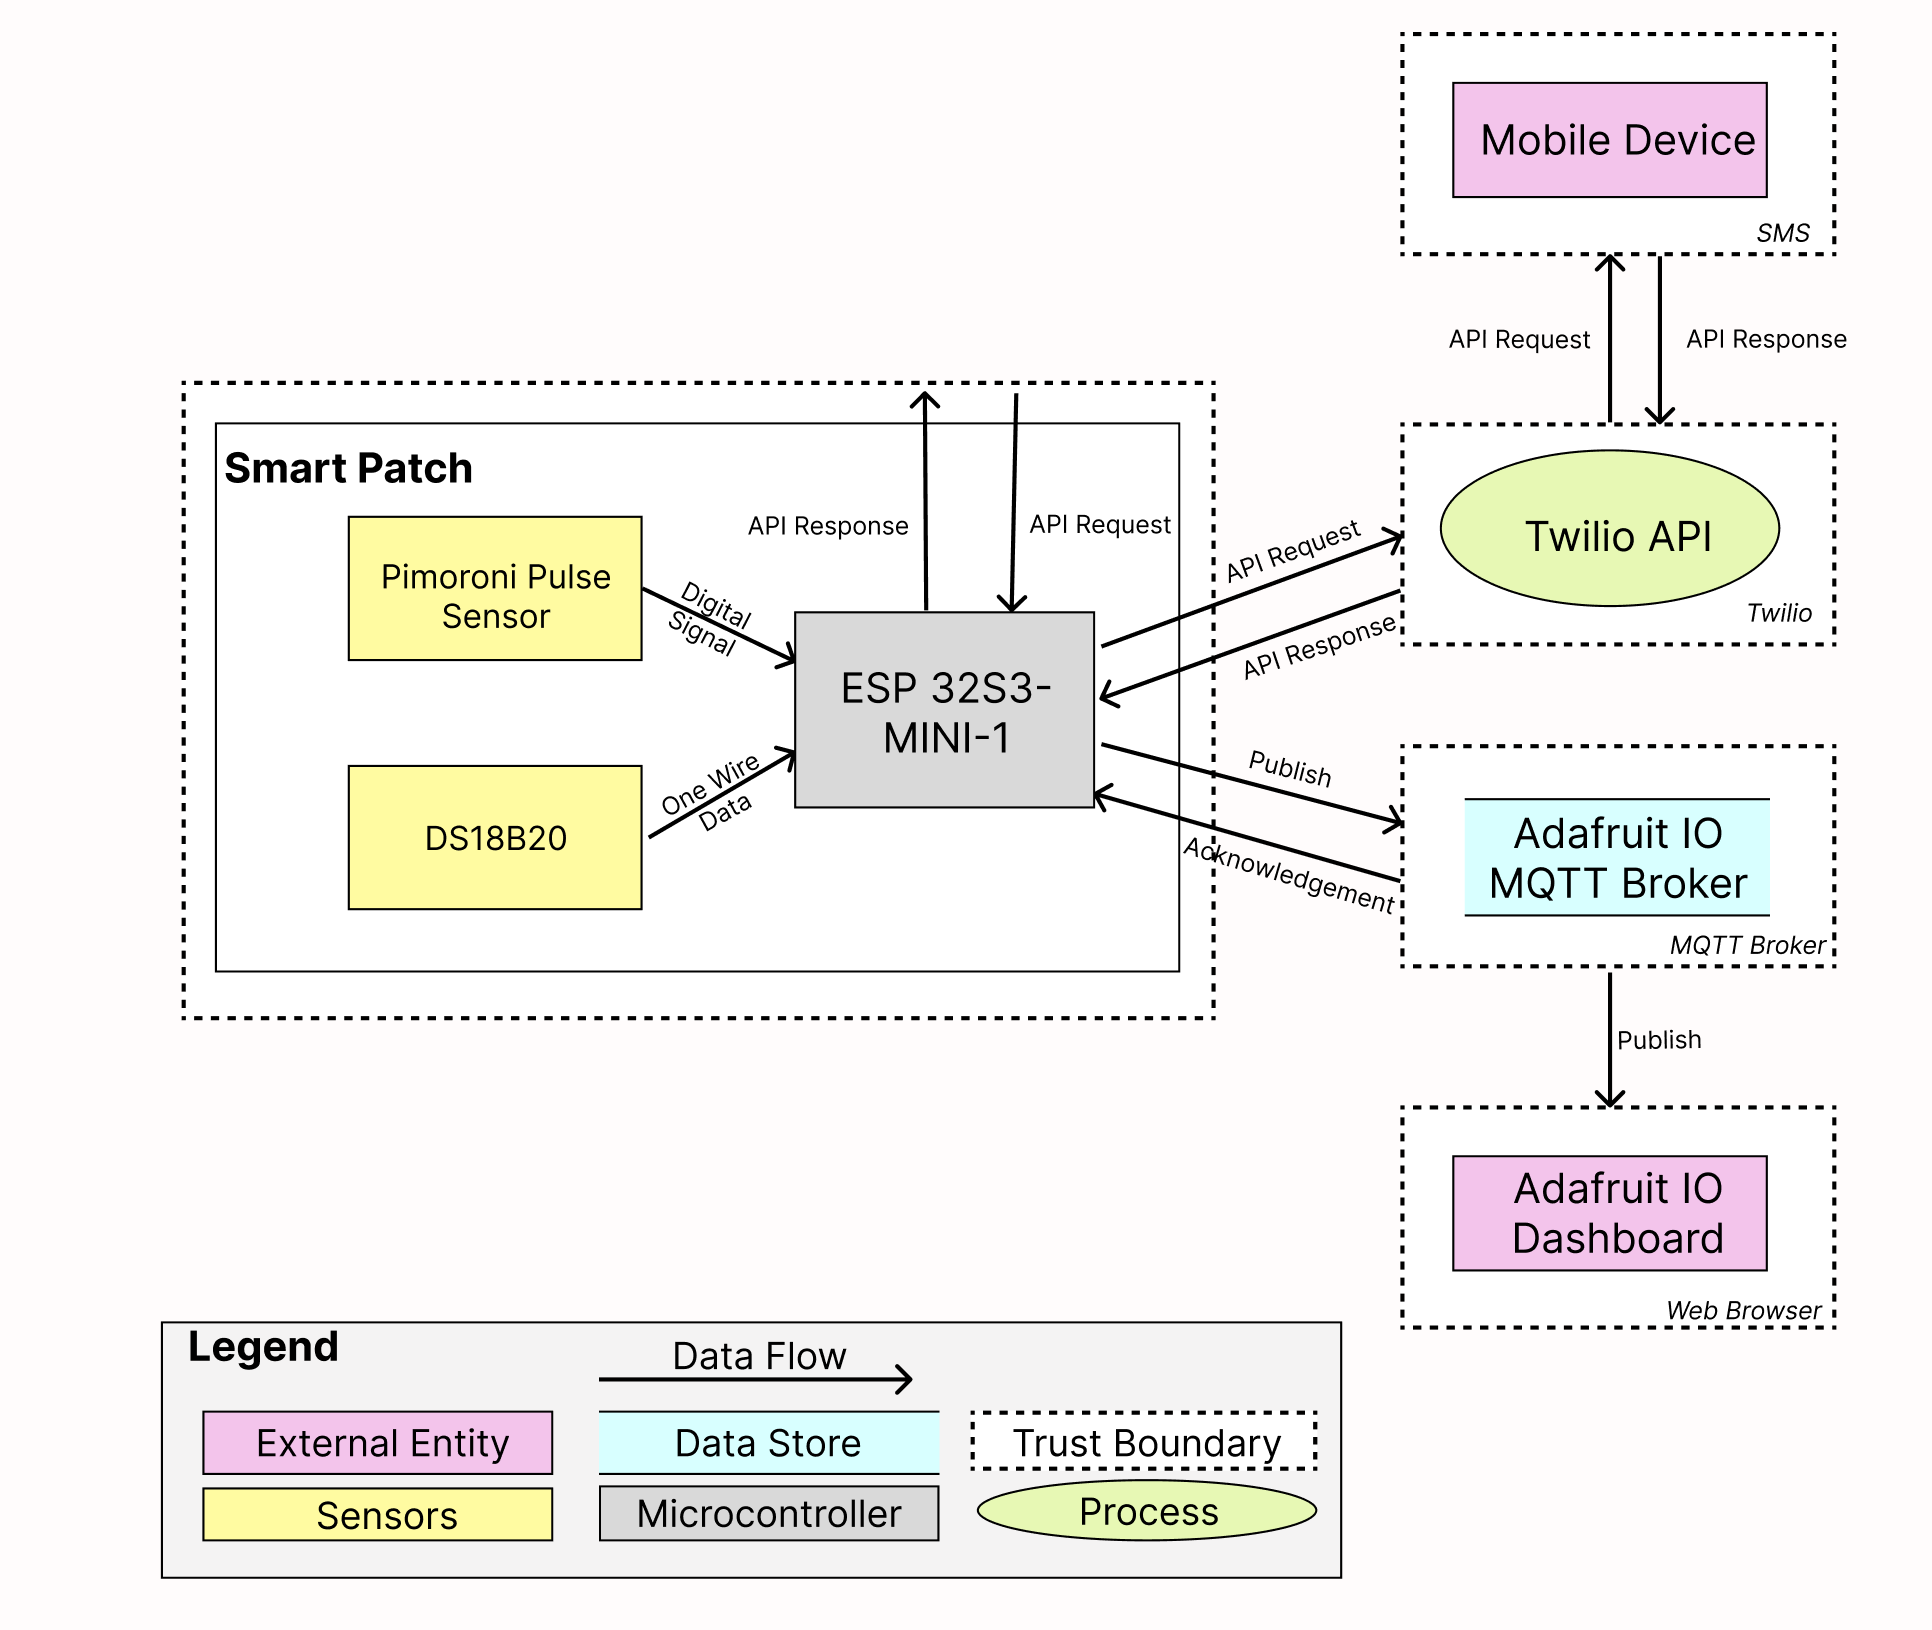
\includegraphics[width=1\linewidth]{images/system-design-data-flow-smart-patch.png}
    \caption{Data Flow Diagram 2}
    \label{fig:dfd-2}
\end{figure}


\newpage
\section{Database Design}
The database is designed using MySQL and is hosted on Google Cloud, leveraging the platform's scalable infrastructure to handle the data management needs of the IoT ecosystem. With a focus on relational integrity and query efficiency, the database schema is structured to support the platform's core functionalities: user management, device tracking, and real-time data analytics.\\

\noindent Figure \ref{fig:database-diagram} provides a visual representation of the relational models and their interconnections. It illustrates the foreign key relationships and cardinality between tables, reflecting the database's normalized design that promotes data integrity and reduces redundancy.\\ \\ \\ 

\begin{figure}[!h]
    \centering
    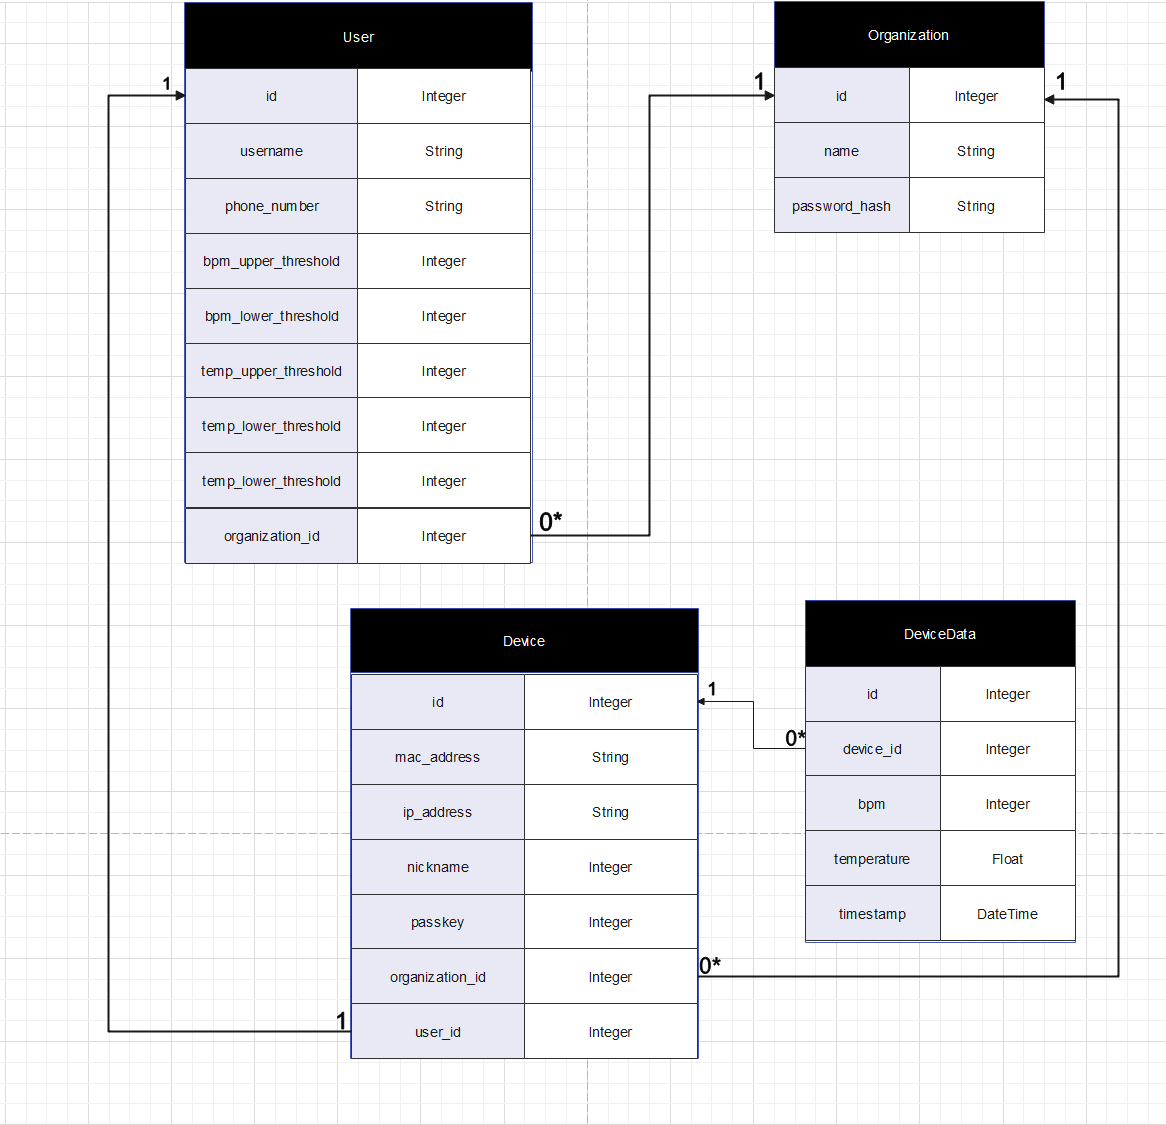
\includegraphics[width=\linewidth]{images/database-obj-relation.png}
    \caption{Database Diagram}
    \label{fig:database-diagram}
\end{figure}

\noindent The main entities of the database are:
\subsection{Organizations}
Organizations form the top hierarchical level within VitalMonitor, representing entities that manage a collection of users and devices. The organization's model features fields for identification, authentication, and relationships to devices and users. Robust security measures are implemented, including hashed passwords using bcrypt to safeguard access credentials.

\subsection{Devices}
The Device model is a representation of physical IoT devices in the system, uniquely identified by a MAC address. Devices are associated with an organization and optionally linked to a specific user. Each device holds a passkey for secure communications and maintains a record of health data streams through its one-to-many relationship with the DeviceData model.

\subsection{Users}
Users are associated with an organization and have a direct connection to a single device. The User model contains contact information and configurable thresholds for health metrics, enabling personalized monitoring and alerts.

\subsection{DeviceData}
The DeviceData model captures the essence of IoT functionality within VitalMonitor. It stores time-series data from IoT devices, including heart rate (bpm) and temperature readings, with precise timestamps. This model ensures that vital health data is recorded, enabling historical data analysis and real-time monitoring.\\

\noindent The database's design is crafted to be intuitive and efficient, facilitating straightforward interactions for the system's backend services. By adopting this structured approach, VitalMonitor ensures fast retrieval of data, which is paramount for real-time applications, while also maintaining the flexibility to scale and adapt to future requirements. \\

\noindent The firmware is designed to handle the exchange of threshold parameters and user information with the middleware. If the measured bpm or temperature exceeds the set thresholds, the device utilizes the Twilio API to dispatch an SMS to a designated emergency contact.

\section{Smart Patch (Firmware) Design}

The firmware for Smart Patch is an ESP32S3-MINI-1 microcontroller. It constitutes the operational bedrock for interfacing with the hardware sensors and executing the device's logic. It is meticulously programmed to manage sensor data acquisition, device control, network communication, and emergency alerting functionalities.

\subsection{Hardware Components}
The device is equipped with a DS18B20 temperature sensor and a Pimoroni Pulse Sensor, tasked with measuring the user's body temperature and heart rate, respectively. The temperature sensor circuit includes a 4.3k\(\Omega\) pull-up resistor essential for accurate signal readings. Similarly, a 1k\(\Omega\) resistor is employed in the LED circuit to indicate the device's operational status. Activation of the sensors and publication of data is controlled by a user-operated push button which toggles the data transmission process, with an LED serving as a visual indicator for the current state—lit when data is being sent and unlit otherwise. The device is powered by a LiPo battery, ensuring portability and convenience.


\subsection{Hardware Circuit Diagram}
A detailed circuit diagram is shown in figure \ref{fig:full-circuit-diagram} outlines the wiring and connections of all components. This showcases the precise electrical relationships and configurations necessary for optimal performance. This diagram serves as a guide for the physical assembly of the hardware components. In the diagram 3V connection is shown using a red wire and ground (or GND) connection is shown using a blue wire. Legend to this figure is provided in figure \ref{fig:legend-circuit}. \\ \\
\begin{figure}[h!]
    \centering
    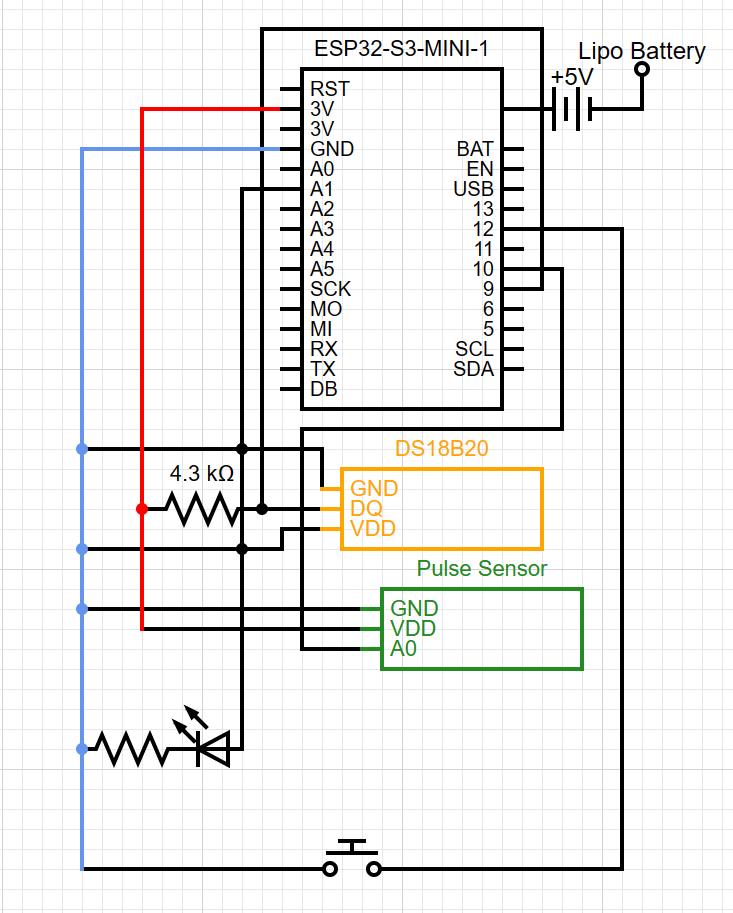
\includegraphics[width=0.8\linewidth]{images/full-circuit-diagram-2.png}
    \caption{Circuit Diagram of Smart Patch}
    \label{fig:full-circuit-diagram}
\end{figure}
\begin{figure}[h!]
    \centering
    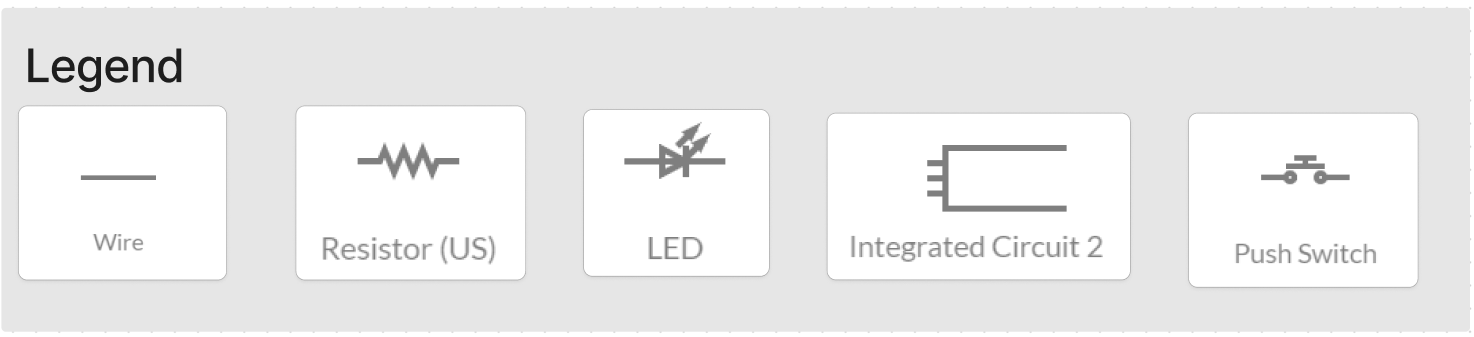
\includegraphics[width=1\linewidth]{images/legend-circuit.png}
    \caption{Legend for circuit diagram}
    \label{fig:legend-circuit}
\end{figure}

\noindent Adafruit IO Dashboard is also designed to get data directly from the firmware for testing purposes. This dashboard allows lightweight transfer of data and allows visualisation (eg., time-series graph) of the health data - which is useful to see how efficiently the data is read by the sensors.  Check Appendix \ref{app:adafruit} for more details on Adafruit IO Dashboard and how it works.


\newpage
\section{Middleware Design}

The Middleware within VitalMonitor serves as the central communication hub, orchestrating interactions among the platform's components. It acts as the pivotal component that integrates dashboards, databases, and smart patches, ensuring seamless functionality and cohesion.

\begin{figure}[!h]
    \centering
    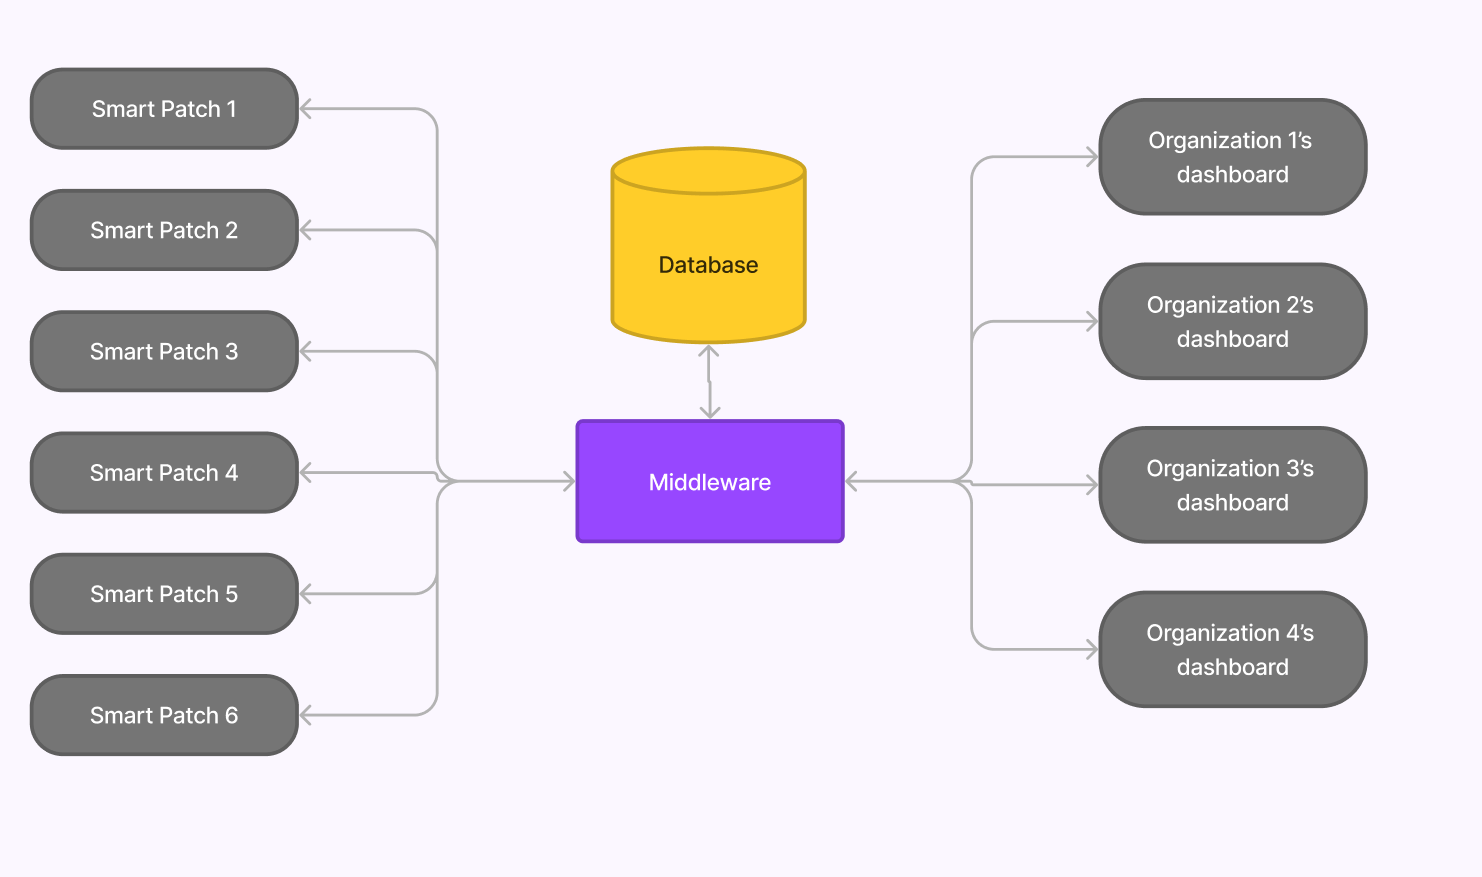
\includegraphics[width=1\linewidth]{images/compressed-data-flow.png}
    \caption{Middleware}
    \label{fig:dfd-3}
\end{figure}

\subsection{Architecture and Responsibility}
The Middleware, designed as an Application Server Middleware (ASM), bears the responsibility of overseeing vital functions necessary for the optimal operation of the VitalMonitor platform. It shoulders tasks such as processing requests, enforcing business logic, managing data, and facilitating communication between the different components of the system.\\

\noindent Additionally, following a microservices-like architecture, the Middleware offers four primary services to the system:

\begin{itemize}
    \item Session Management Service
    \item User and Device Management Service
    \item Data Ingestion Service
    \item Data Retrieval Service
\end{itemize}

\noindent This is done in such a way because when the load of number of devices and dashboard increases, the middleware will not be able to handle it. There fore, in future, isolating the service and having them as their own services along with a load balancer, this allows more controlled and managed data. 

\subsection{Design Principles}
Several key principles guided the design of the Middleware:
\begin{enumerate}
    \item \textbf{Communication Hub:}
The Middleware is designed to be a central communication hub. It is responsible for the uninterrupted flow of data between devices and the user interface. It acts as the API Gateway, receiving API calls from the dashboard, interpreting them, and routing these to the appropriate services or data stores.
\item \textbf{Abstraction:}
The Middleware is designed to provide a level of abstraction that simplifies interactions between the user interface and the system's backend. It abstracts the complexities of the underlying database structures and device communication protocols from the end-user, presenting a simple and coherent interface to the dashboard and using of smart patch.
\item \textbf{Data Management:}
The Middleware is designed to provide robust data management. It provides a secure and efficient gateway to the database, handling transactions, query processing, and data synchronization. This ensures data integrity and consistent state across the platform, even as it scales.
\item \textbf{Unified Connection for Multiple Entities:}
The Middleware is designed with a comprehensive routing and authentication system. This facilitates concurrent connections across multiple dashboards and smart patches. It supports a multiplexed network structure where each entity is uniquely identified and managed, maintaining a coherent state across the ecosystem.
\end{enumerate}

By adhering to these principles, the Middleware embodies a pivotal component within the VitalMonitor ecosystem - fostering efficient communication, seamless operation, and scalable growth.

\section{Dashboard Design}

The VitalMonitor dashboard is specifically designed to serve as a centralized control panel for organization administrators, enabling them to efficiently manage healthcare professionals' data. This platform facilitates real-time monitoring and management of user profiles and devices, allowing admins to set health thresholds, add or delete users, and assign devices. The dashboard is crafted to cater to the specific needs of health organization administrators, providing them with intuitive tools to enhance operational efficiency and patient care.

\subsection{Technology and Tools}
The dashboard is designed using Flask, a micro web framework that offers flexibility and simplicity for server-side logic. Flask's lightweight and modular nature makes it an ideal choice for constructing a responsive and efficient web application. For the frontend, HTML, CSS, and JavaScript are employed to create a dynamic and interactive user interface that responds to the administrators' operational needs effectively.

\subsection{Design Pattern}


\subsubsection{Decorator Pattern}
The use of the Decorator Pattern is fundamental in the design of our Flask application, especially in managing route associations and enhancing function capabilities without modifying their core responsibilities:

\begin{itemize}
    \item \textbf{Routing}: Utilizing Flask's @app.route() decorator simplifies the mapping of HTTP requests to Python functions, making the association between URL routes and server-side logic clear and maintainable.
    \item \textbf{Custom Decorators}:  Custom decorators are designed to manage user session and authentication checks. These intercept and verify requests to ensure user authentication before accessing specific functionalities, thus enhancing security and user management efficiency.
\end{itemize}

\subsubsection{Model View Controller-like Structure}
While Flask does not enforce an MVC architecture, the design of the dashboard subtly incorporates elements of this pattern, enhancing clarity and separation within the application:

\begin{itemize}
    \item \textbf{Model (M)}: The business logic and data interactions are handled in the background, interfacing with the middleware. This includes user and device management functionalities, where data integrity and operations like add, update, and delete are executed. Middleware provides access to requested data but not the full model and its data directly, for an additional layer of security. 
    \item \textbf{View (V)}: The presentation layer is managed through Flask’s template system. HTML templates are rendered based on the data processed by the controllers, providing a user-friendly interface for interaction. Templates for pages like \textit{add\_device.html} and \textit{user\_page.html} define how data is presented and ensure a consistent user experience.
    \item \textbf{Controller (C)}: Flask routes act as controllers, orchestrating the application's response to user inputs and interactions. They process incoming requests, call the appropriate model functions, and determine the correct views to render, completing the user request lifecycle.
\end{itemize}

\newpage
\subsection{User Flow}
The user flow diagram (Figure \ref{fig:user-flow}) visually represents the navigational pathway administrators take through the dashboard. It highlights the sequence of interactions from login to detailed device and user management.

\begin{figure}[!h]
    \centering
    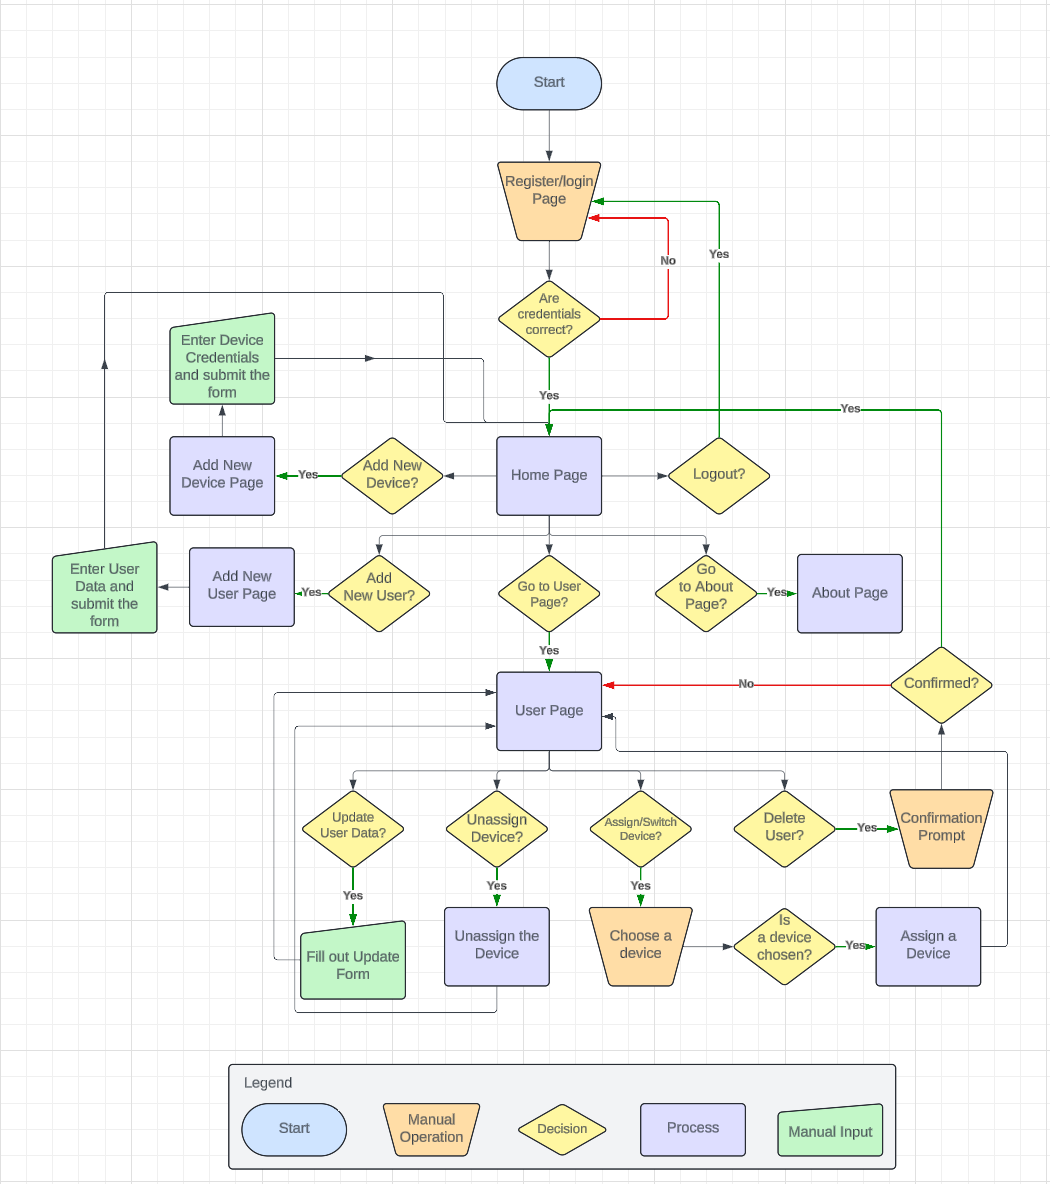
\includegraphics[width=1\linewidth]{images/user-flow.png}
    \caption{User Flow Diagram for Dashboard}
    \label{fig:user-flow}
\end{figure}

\subsection{Wireframes}
\begin{figure}[!h]
    \centering
    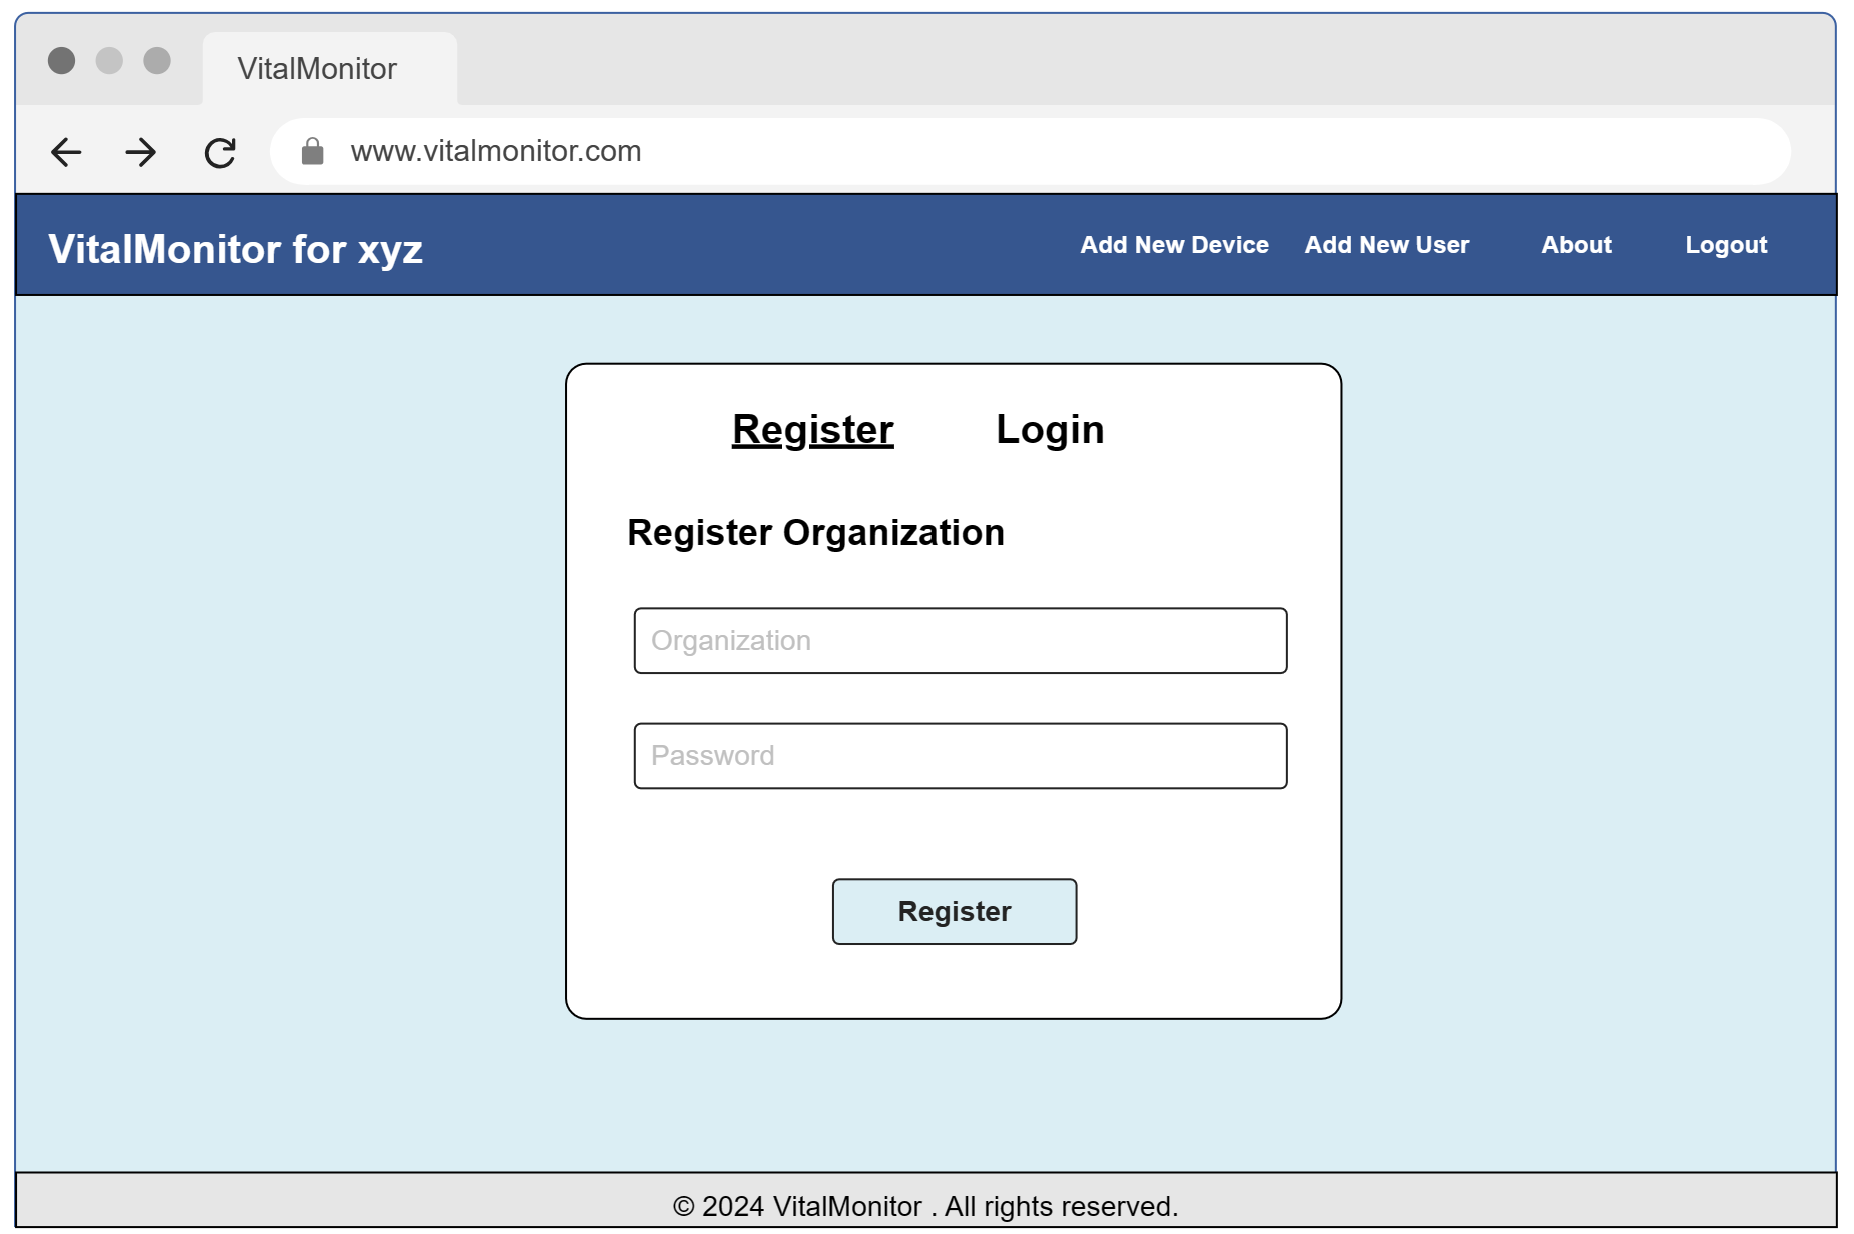
\includegraphics[width=0.87\linewidth]{images/register organization.png}
    \caption{Landing Page to register/login}
    \label{fig:wf-4}
\end{figure}

\begin{figure}[!h]
    \centering
    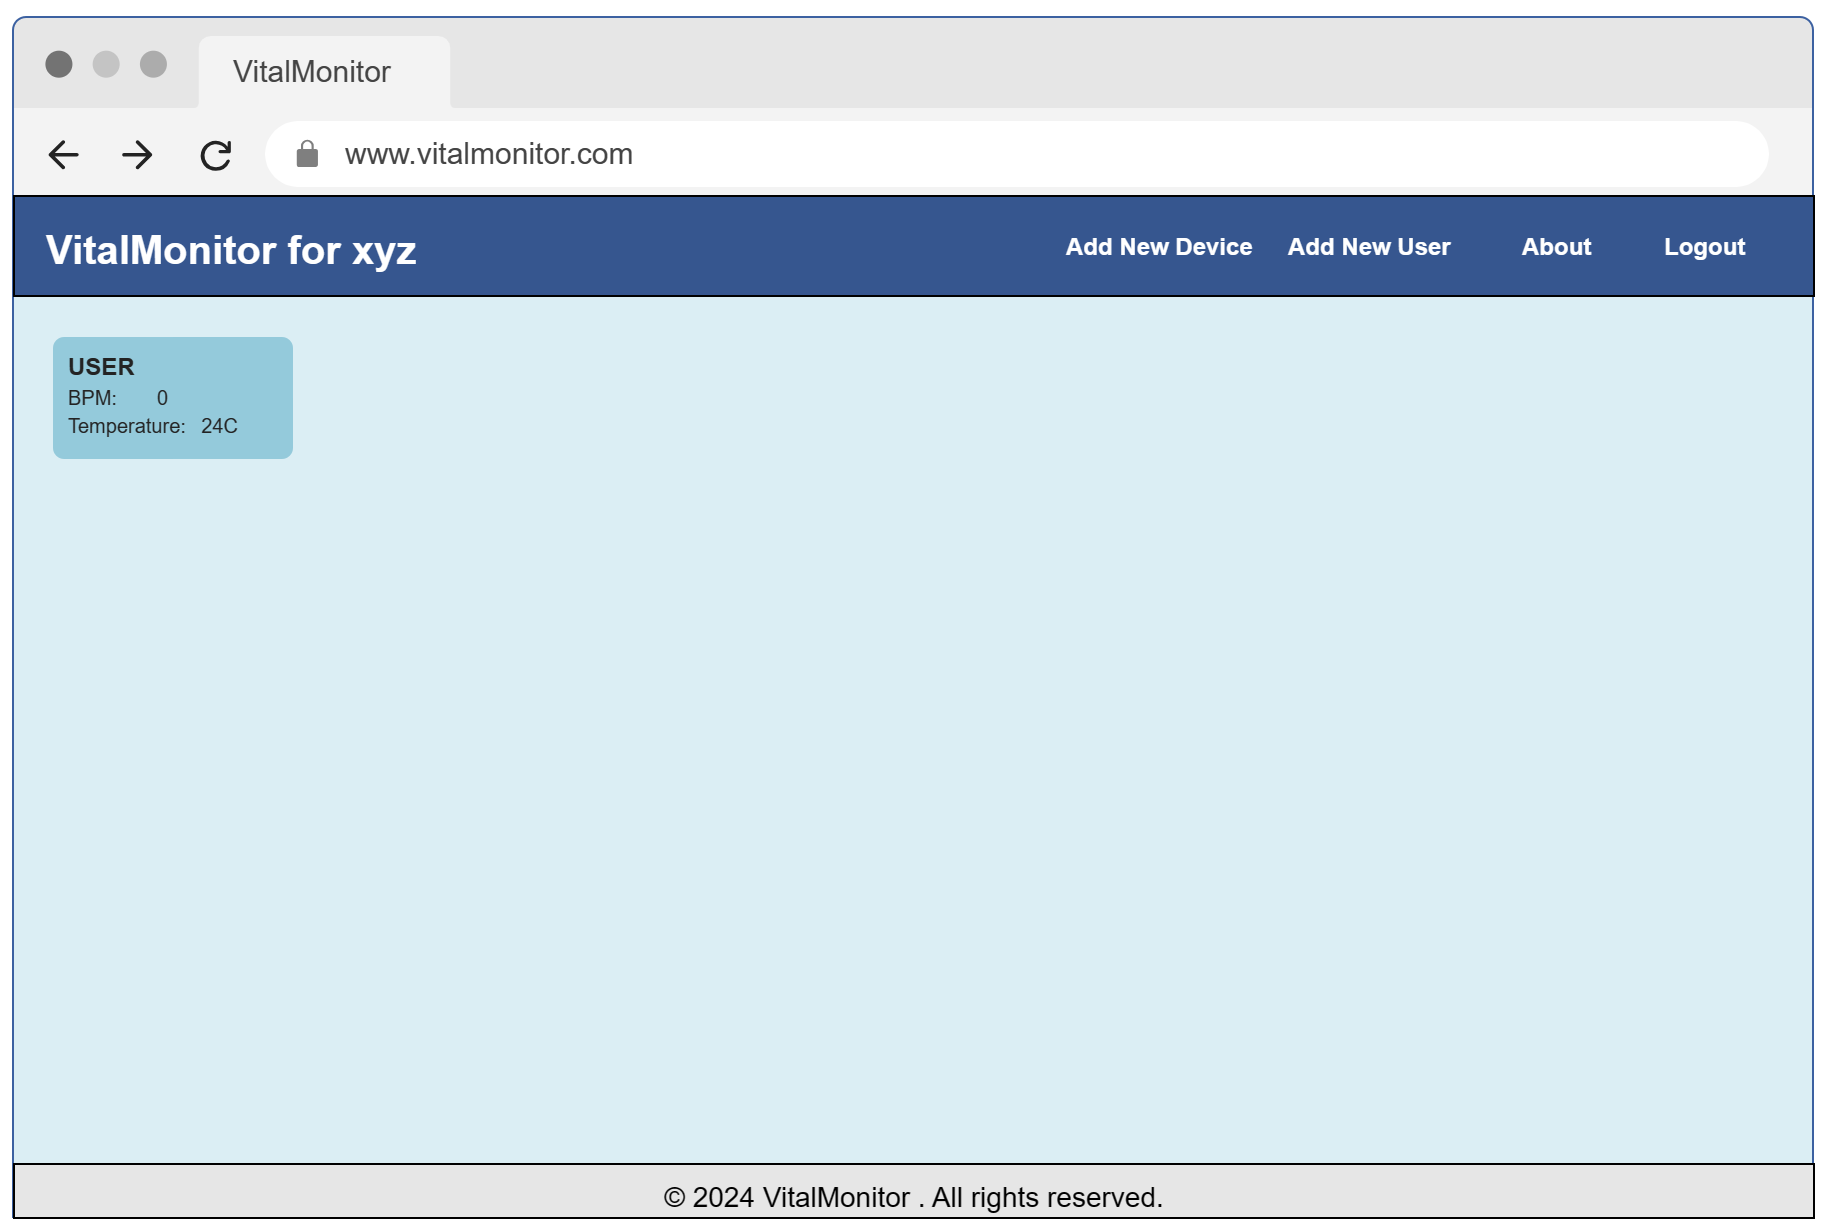
\includegraphics[width=0.87\linewidth]{images/home.png}
    \caption{Home Page}
    \label{fig:wf-3}
\end{figure}

\begin{figure}[!h]
    \centering
    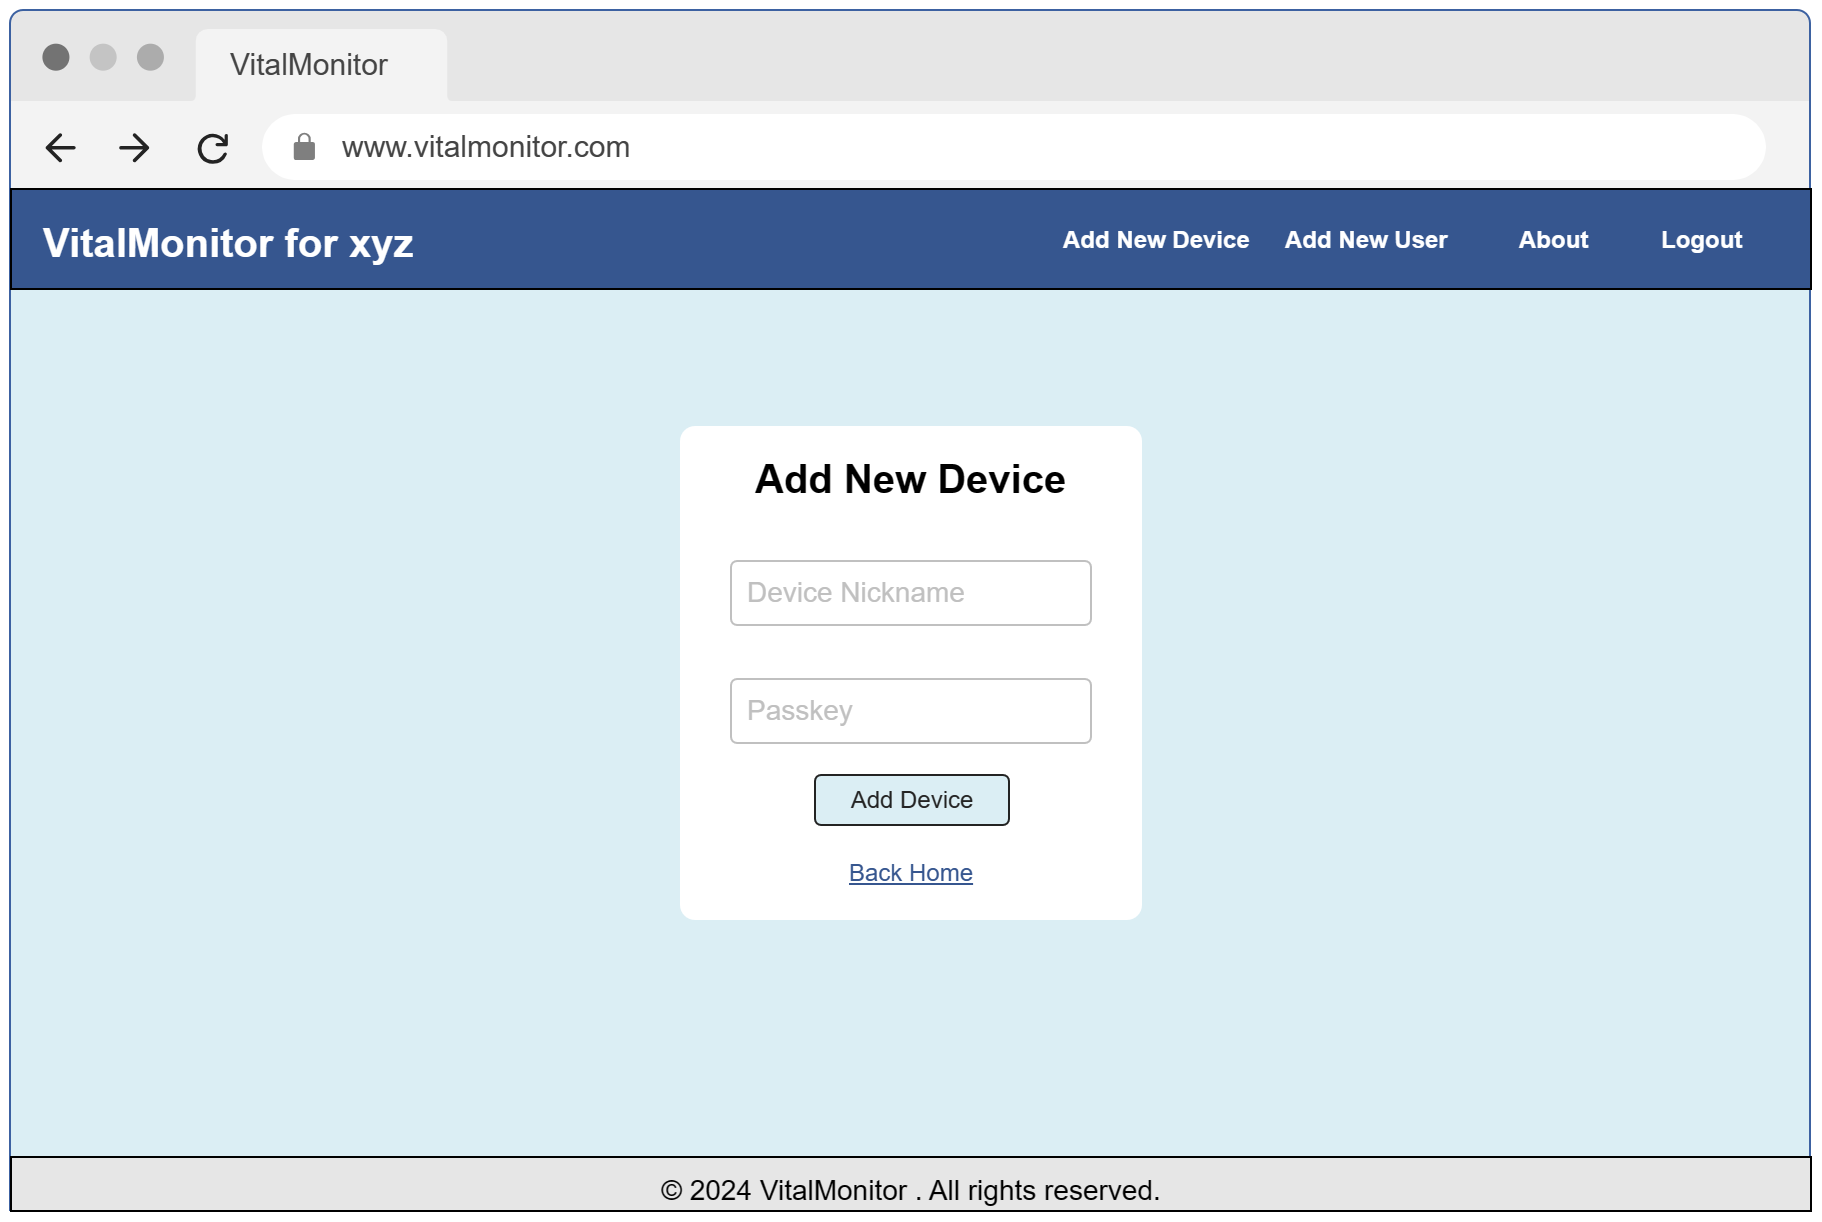
\includegraphics[width=0.9\linewidth]{images/Addnewdevice.png}
    \caption{Add New Device page}
    \label{fig:wf-1}
\end{figure}
\begin{figure}[!h]
    \centering
    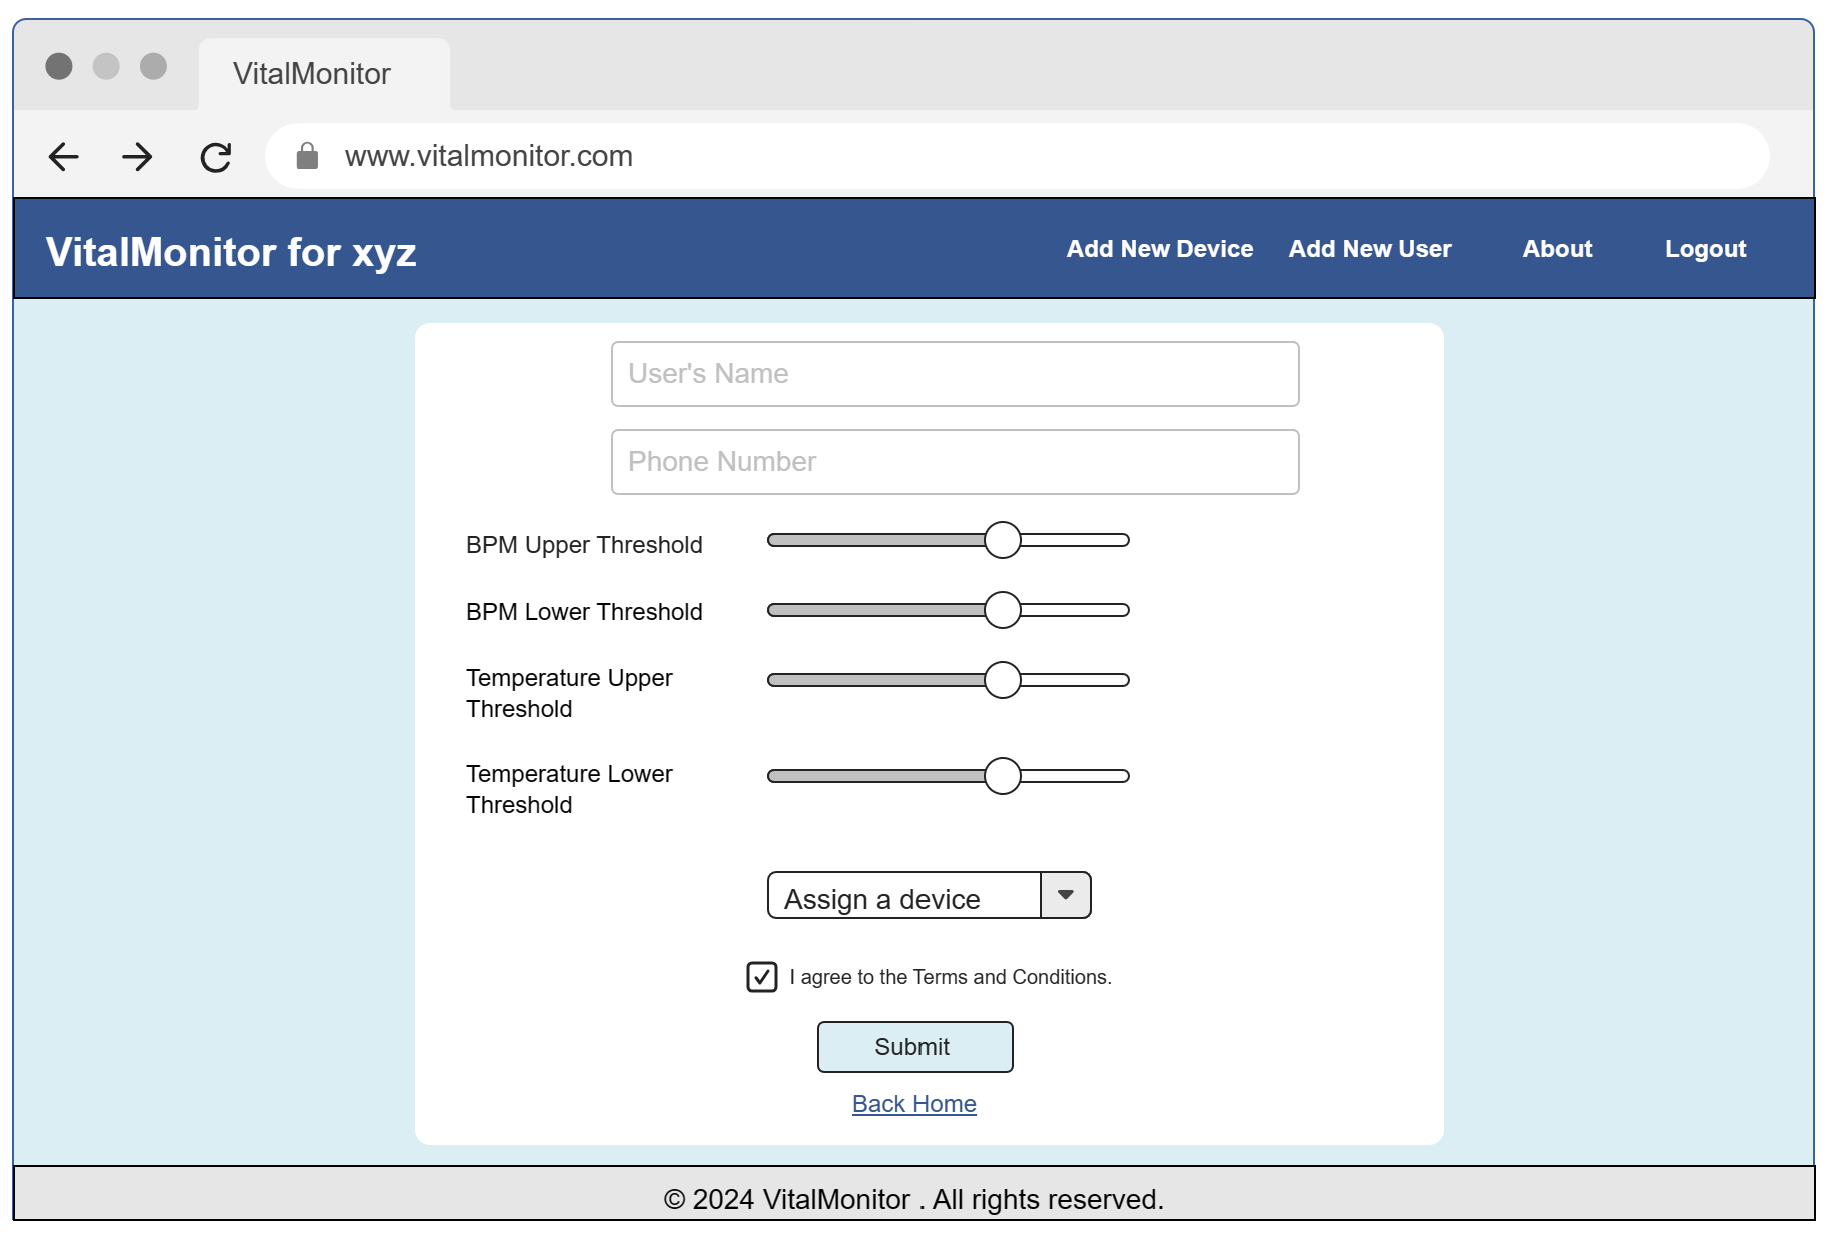
\includegraphics[width=0.9\linewidth]{images/addnewuser.png}
    \caption{Add New User Page}
    \label{fig:wf-2}
\end{figure}

\begin{figure}[!h]
    \centering
    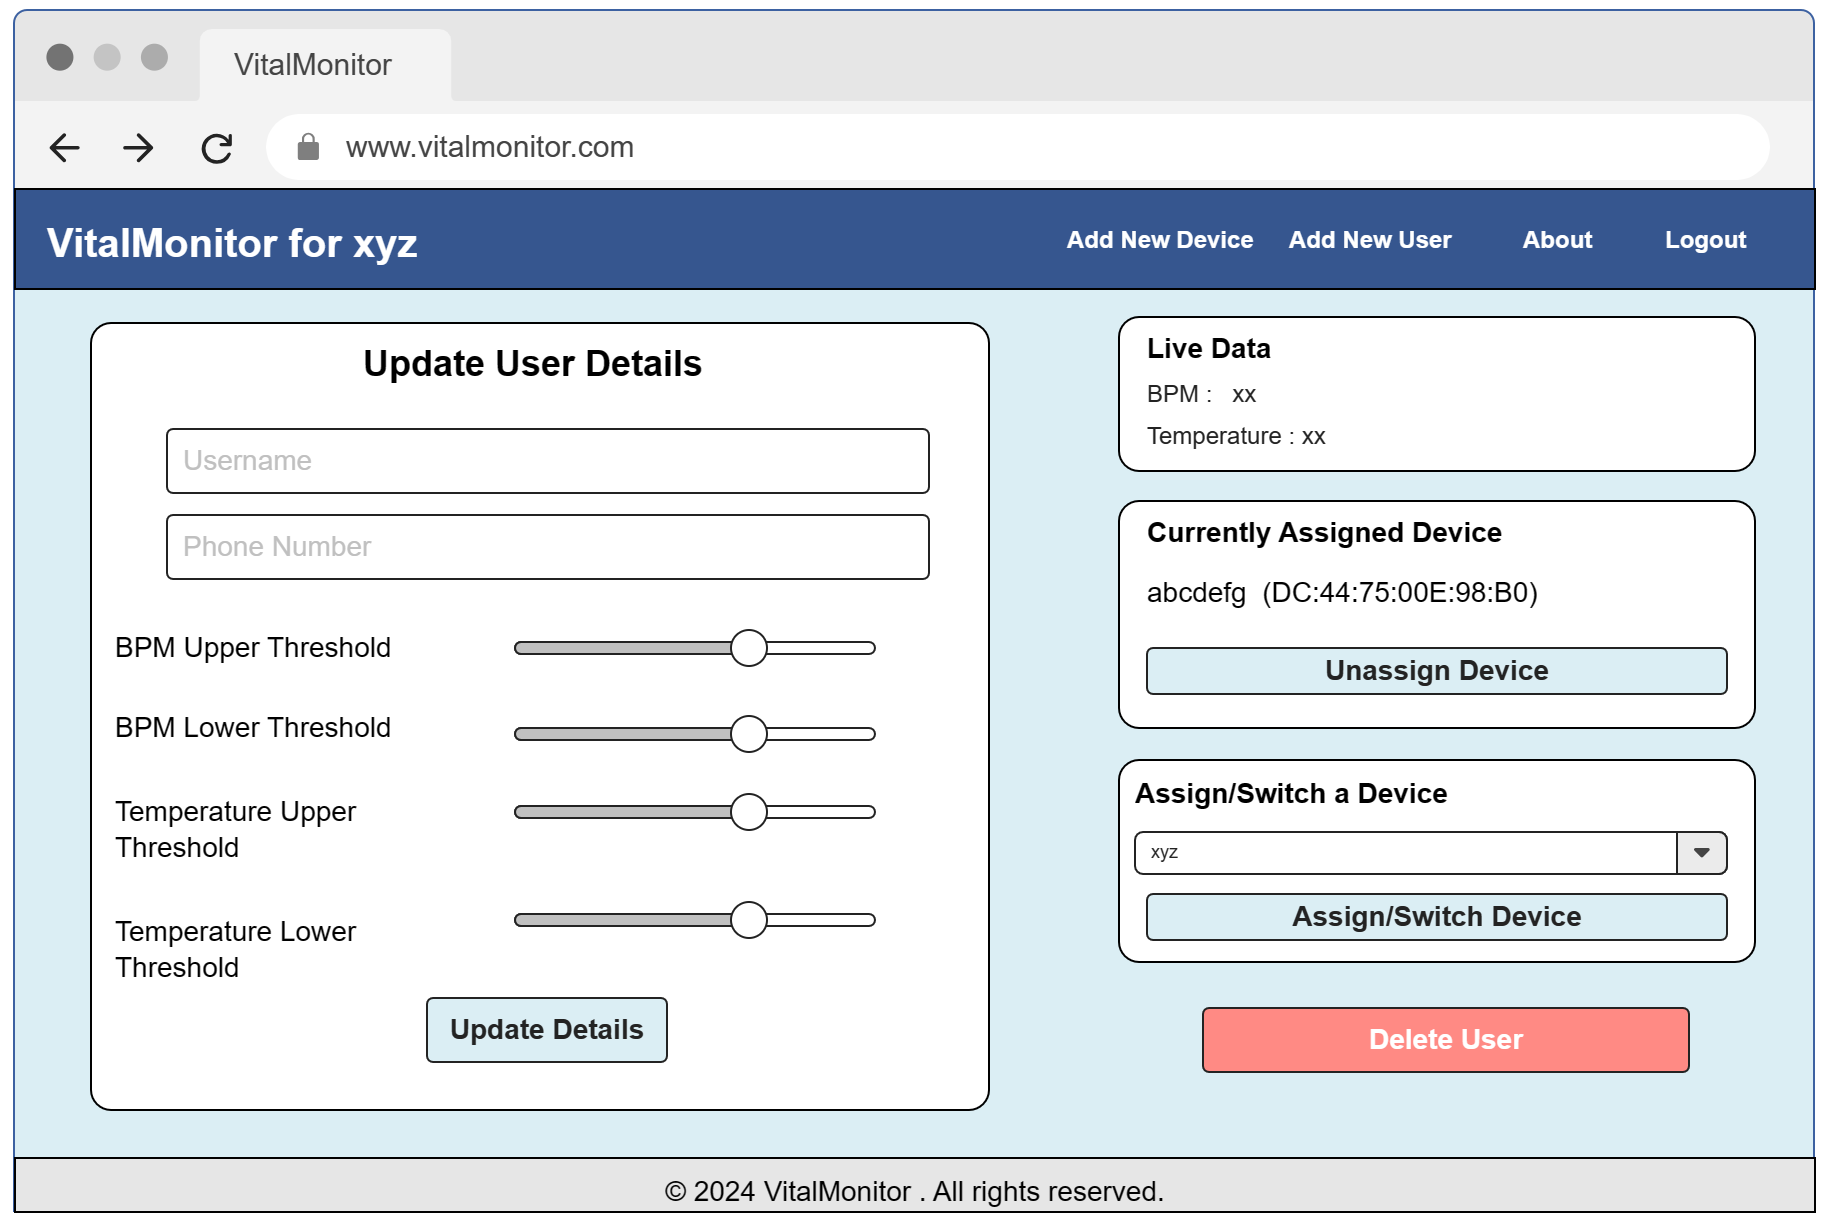
\includegraphics[width=0.9\linewidth]{images/update user details.png}
    \caption{User Page}
    \label{fig:wf-5}
\end{figure}
\begin{figure}[!h]
    \centering
    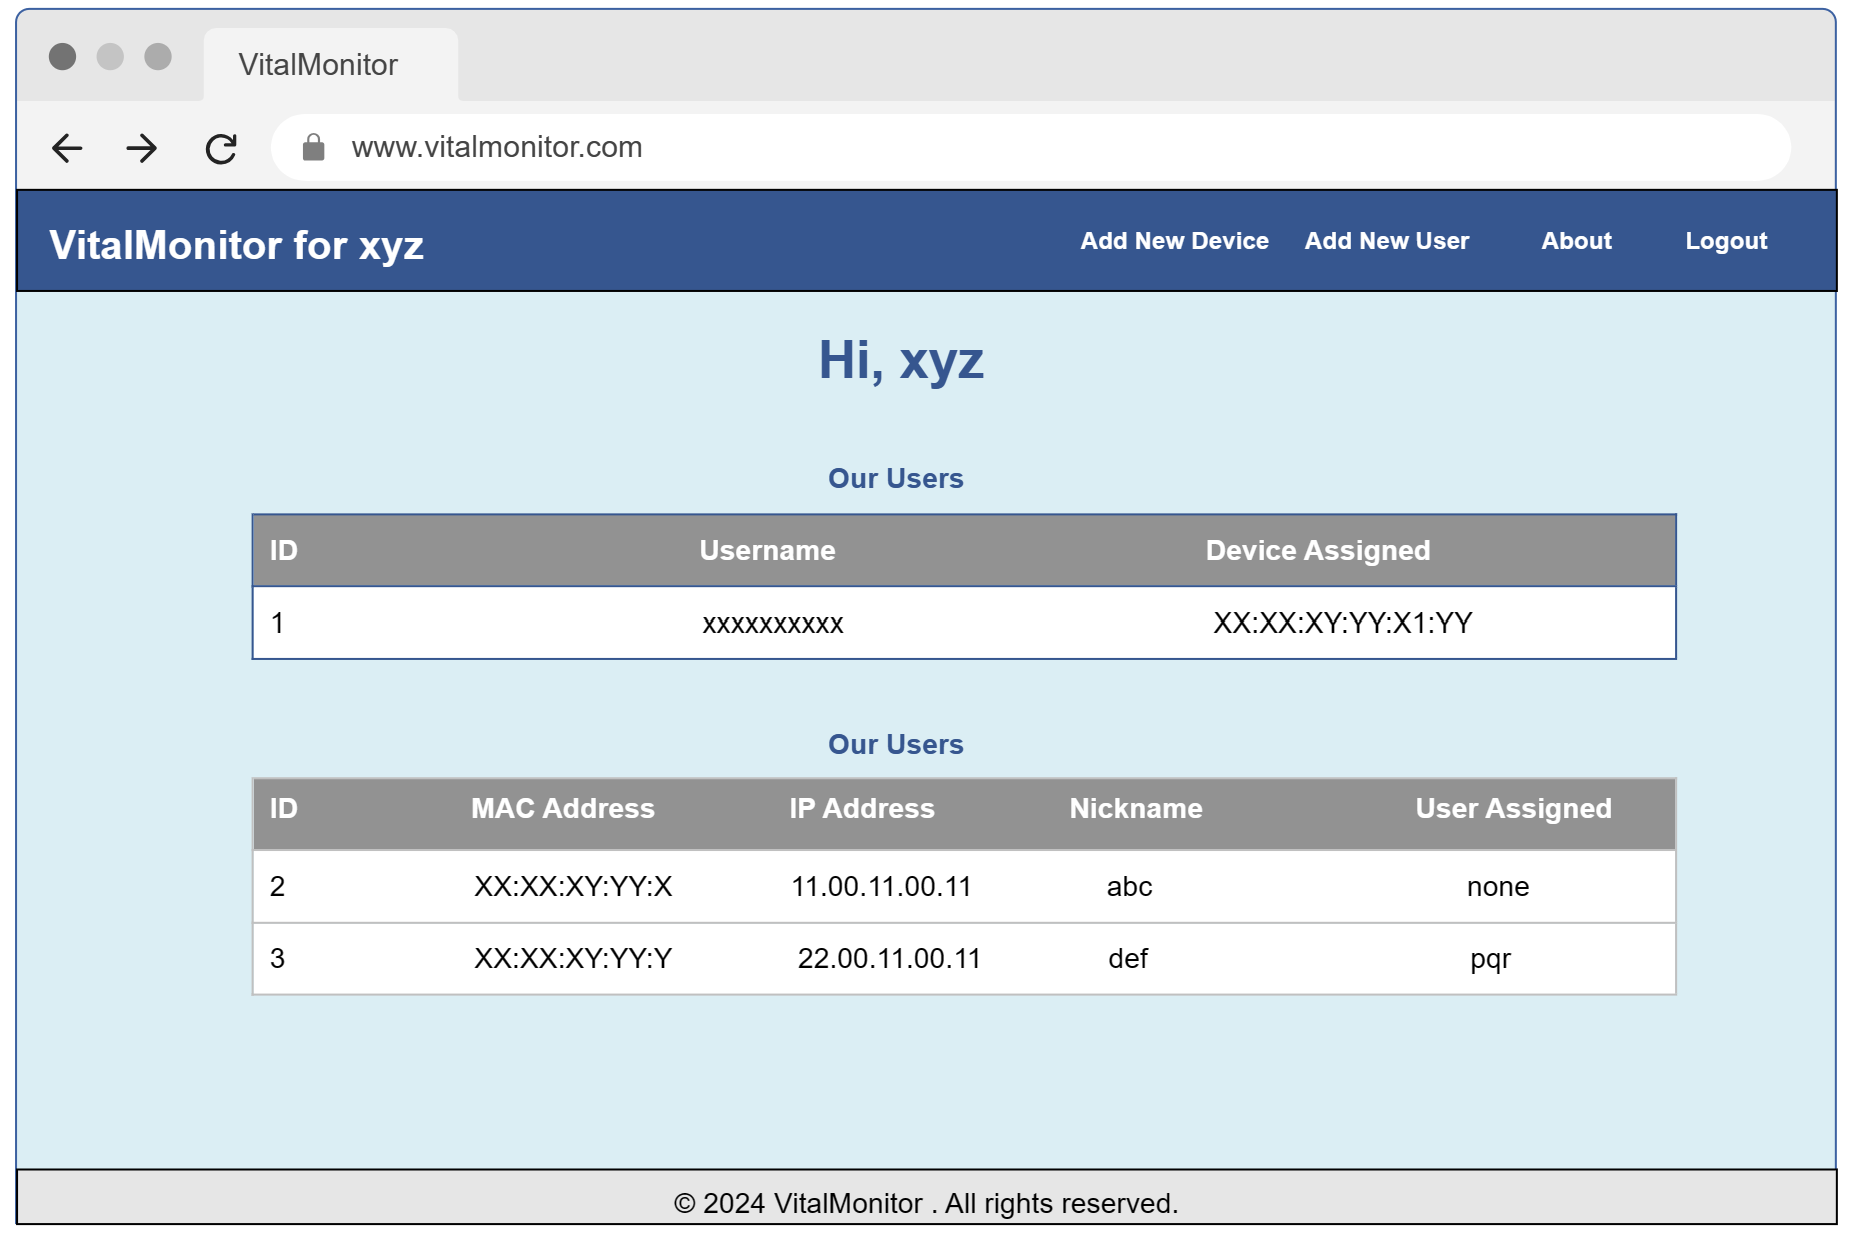
\includegraphics[width=0.9\linewidth]{images/VitalMonitor.png}
    \caption{About Page}
    \label{fig:wf6}
\end{figure}


\section{Network Communication and API Design}
VitalMonitor's networking layer is designed to enable robust and efficient interactions between front-end applications, back-end services, and IoT devices. By utilizing RESTful principles and leveraging the JSON data format, the system ensures streamlined data exchange and functionality that scales effectively with the demands of healthcare monitoring. Along with it, Smart Patches are designed to create their own Asyncronous Web Servers to facilitate transmission of data. Additionally, they are designed to use MQTT Protocol to publish data on Adafruit IO Dashboard.\\

\subsection{API and API Endpoints}
The API endpoints of VitalMonitor are meticulously designed to reflect a resource-oriented approach, enabling straightforward CRUD operations. Here’s a closer look at the design:

\begin{itemize}
    \item Structured for Simplicity and Efficiency: Each endpoint is crafted to represent and manipulate a distinct entity, such as users or devices, simplifying interactions and reducing complexity.
    \item Consistent Data Format: The system exclusively use JSON for all exchanges, ensuring compatibility and ease of development across various platforms.
    \item Stateless Operations: Ensuring each request is self-contained,  the APIs maintains statelessness, which is key to enhancing the scalability and reliability of distributed systems.
\end{itemize}

There are multiple API endpoints for each of the components of the system :\\

\subsubsection{Middleware:}
\begin{longtable}{|p{5cm}|p{1.5cm}|p{7.5cm}|}
\caption{API Endpoints for Middleware} \label{tab:api_endpoints} \\
\hline
\textbf{Endpoint} & \textbf{Method} & \textbf{Description} \\ \hline
\endfirsthead
\multicolumn{3}{c}%
{\tablename\ \thetable\ -- \textit{Continued from previous page}} \\
\hline
\textbf{Endpoint} & \textbf{Method} & \textbf{Description} \\ \hline
\endhead
\hline \multicolumn{3}{r}{\textit{Continued on next page}} \\
\endfoot
\hline
\endlastfoot

/register & POST & Register a new organization with name and password. \\ \hline
/login & POST & Authenticate organization credentials. \\ \hline
/add-new-user & POST & Add a new user to an organization, specifying necessary personal and health threshold details. \\ \hline
/add-new-device & POST & Add or update a device in the system, specifying details like MAC address and IP address. \\ \hline
/associate-device & POST & Associate a device with an organization using device nickname and passkey. \\ \hline
/assign-device-to-user & POST & Assign a device to a specific user, linking it with user ID and device ID. \\ \hline
/unassign-device/\{device\_id\}/\{user\_id\} & POST & Unassign a device from a user, removing all associated user details from the device. \\ \hline
/update-user-details & POST & Update details for an existing user, including contact information and health thresholds. \\ \hline
/get-device-data/\{device\_id\} & GET & Stream real-time data from a specific device. \\ \hline
/save-device-data & POST & Save data received from a device to the database. \\ \hline
/delete-device/\{device\_id\} & DELETE & Remove a device and all its associated data from the system. \\ \hline
/delete-user/\{user\_id\} & DELETE & Remove a user and all their associated details from the system. \\ \hline
/delete-organization/\{organization\_id\} & DELETE & Remove an entire organization and all associated users, devices, and data. \\ \hline
/devices & GET & Retrieve all devices associated with an organization. \\ \hline
/users & GET & Retrieve all users within an organization. \\ \hline
/user/\{user\_id\} & GET & Retrieve detailed information about a specific user. \\ \hline
\end{longtable}

\subsubsection{Dashboard:}
\begin{longtable}{|p{5cm}|p{1.5cm}|p{7.5cm}|}
\caption{Dashboard API Endpoints} \label{tab:dashboard_api_endpoints} \\
\hline
\textbf{Endpoint} & \textbf{Method} & \textbf{Description} \\ \hline
\endfirsthead
\multicolumn{3}{c}%
{\tablename\ \thetable\ -- \textit{Continued from previous page}} \\
\hline
\textbf{Endpoint} & \textbf{Method} & \textbf{Description} \\ \hline
\endhead
\hline \multicolumn{3}{r}{\textit{Continued on next page}} \\
\endfoot
\hline
\endlastfoot

/register & POST & Registers and logs in a new organization. \\ \hline
/login & POST & Authenticates and sets session for an organization. \\ \hline
/ & GET & Displays the main dashboard if logged in. \\ \hline
/register\_login & GET & Shows registration and login portal. \\ \hline
/logout & GET & Logs out and clears session. \\ \hline
/add-device-page & GET & Shows the add device page for logged-in users. \\ \hline
/add-device & POST & Adds a new device and displays status message. \\ \hline
/submit-user-details & GET & Displays unassigned devices for user assignment. \\ \hline
/add-user & POST & Adds a new user and optionally assigns a device. \\ \hline
/user/{user\_id} & GET, POST & Allows updating user details and device assignment. \\ \hline
/device/{device\_id}/update-details & POST & Sends updated user data to a device. \\ \hline
/sendDetails & POST & Receives and updates live BPM and temperature data. \\ \hline
/data-stream & GET & Streams live BPM and temperature data. \\ \hline
/about-us & GET & Displays organization details for logged-in users. \\ \hline
\end{longtable}


\subsubsection{Smart Patch:}
\begin{longtable}{|p{5cm}|p{1.5cm}|p{7.5cm}|}
\caption{Smart Patch API Endpoints} \label{tab:smart_patch_api_endpoints} \\
\hline
\textbf{Endpoint} & \textbf{Method} & \textbf{Description} \\ \hline
\endfirsthead
\multicolumn{3}{c}%
{\tablename\ \thetable\ -- \textit{Continued from previous page}} \\
\hline
\textbf{Endpoint} & \textbf{Method} & \textbf{Description} \\ \hline
\endhead
\hline \multicolumn{3}{r}{\textit{Continued on next page}} \\
\endfoot
\hline
\endlastfoot

/receive-user-details & POST & Receives and stores user details for device assignment, enabling personalized data monitoring and alerts. \\ \hline
/clear-user-details & POST & Clears all user-specific details from the device, effectively unassigning it from a user. \\ \hline
/stop-publishing & GET & Handles request to stop data publishing, which could be triggered remotely via web request. \\ \hline

\end{longtable}

Lastly, feeds will be designed as per MQTT Protocol for sending data to Adafruit IO Dashboard. See Appendix \ref{app:adafruit} for more information.

\newpage
\subsection{Error Handling and Management}
The implemented networking layer should be able to handle different HTTP client and server errors that can occur. The supported errors are: \\

\begin{table}[!h]
\centering
\begin{tabularx}{\textwidth}{|X|X|}
\hline
\textbf{Error Code} & \textbf{Error Descriptions}  \\ \hline
400 & Bad Request \\ \hline
401 & Unauthorised \\ \hline
404 & Not Found \\ \hline
409 & Conflict with current state/resources \\ \hline
500 & Network Errors  \\ \hline
\end{tabularx}
\caption{Supported Error Codes}
\label{tab:error-codes}
\end{table} 

More error conditions can be added in future, if deemed necessary. However, these cover the minimum needed to provide a reliable user experience.



\chapter{Implementation and Testing}

\section{Implementation and Testing Strategy}

The implementation of the VitalMonitor system was orchestrated using Agile methodologies to foster iterative development and continuous integration across all subsystems: the Smart Patch, the Middleware application server, and the Dashboard web application. Beginning with the Smart Patch, the development strategy emphasized incremental builds, each enhancing specific functionalities such as sensor integration, WiFi connectivity, Adafruit IO, and webserver capabilities, with rigorous assessment through a detailed test suite that evaluated each function against predefined test specifications. The development of Smart Patch was divided into 8 iterations or versions - each either adding a new functionality or solving a previous problem. \\

\noindent Following the initial development, the Dashboard was implemented using Flask, HTML, CSS, and JavaScript, supported by an SQLite database for local testing before transitioning to a full integration with the Middleware. This Middleware, also Flask-based, served as the central communication hub, facilitating robust data interactions between the Smart Patch, Dashboard, and a MySQL database hosted on Google Cloud. Applying a consistent test suite approach across all subsystems ensured high standards of functionality and performance were maintained, leading to a seamlessly functioning integrated system upon final assembly. \\

% OPTIONAL
% A gantt chart was made to plan out the project timeline. This is shown in figure \ref{fig:gantt-chart}. This chart was updated at each stage of the project. 

% \begin{figure}[h!]
%     \centering
%     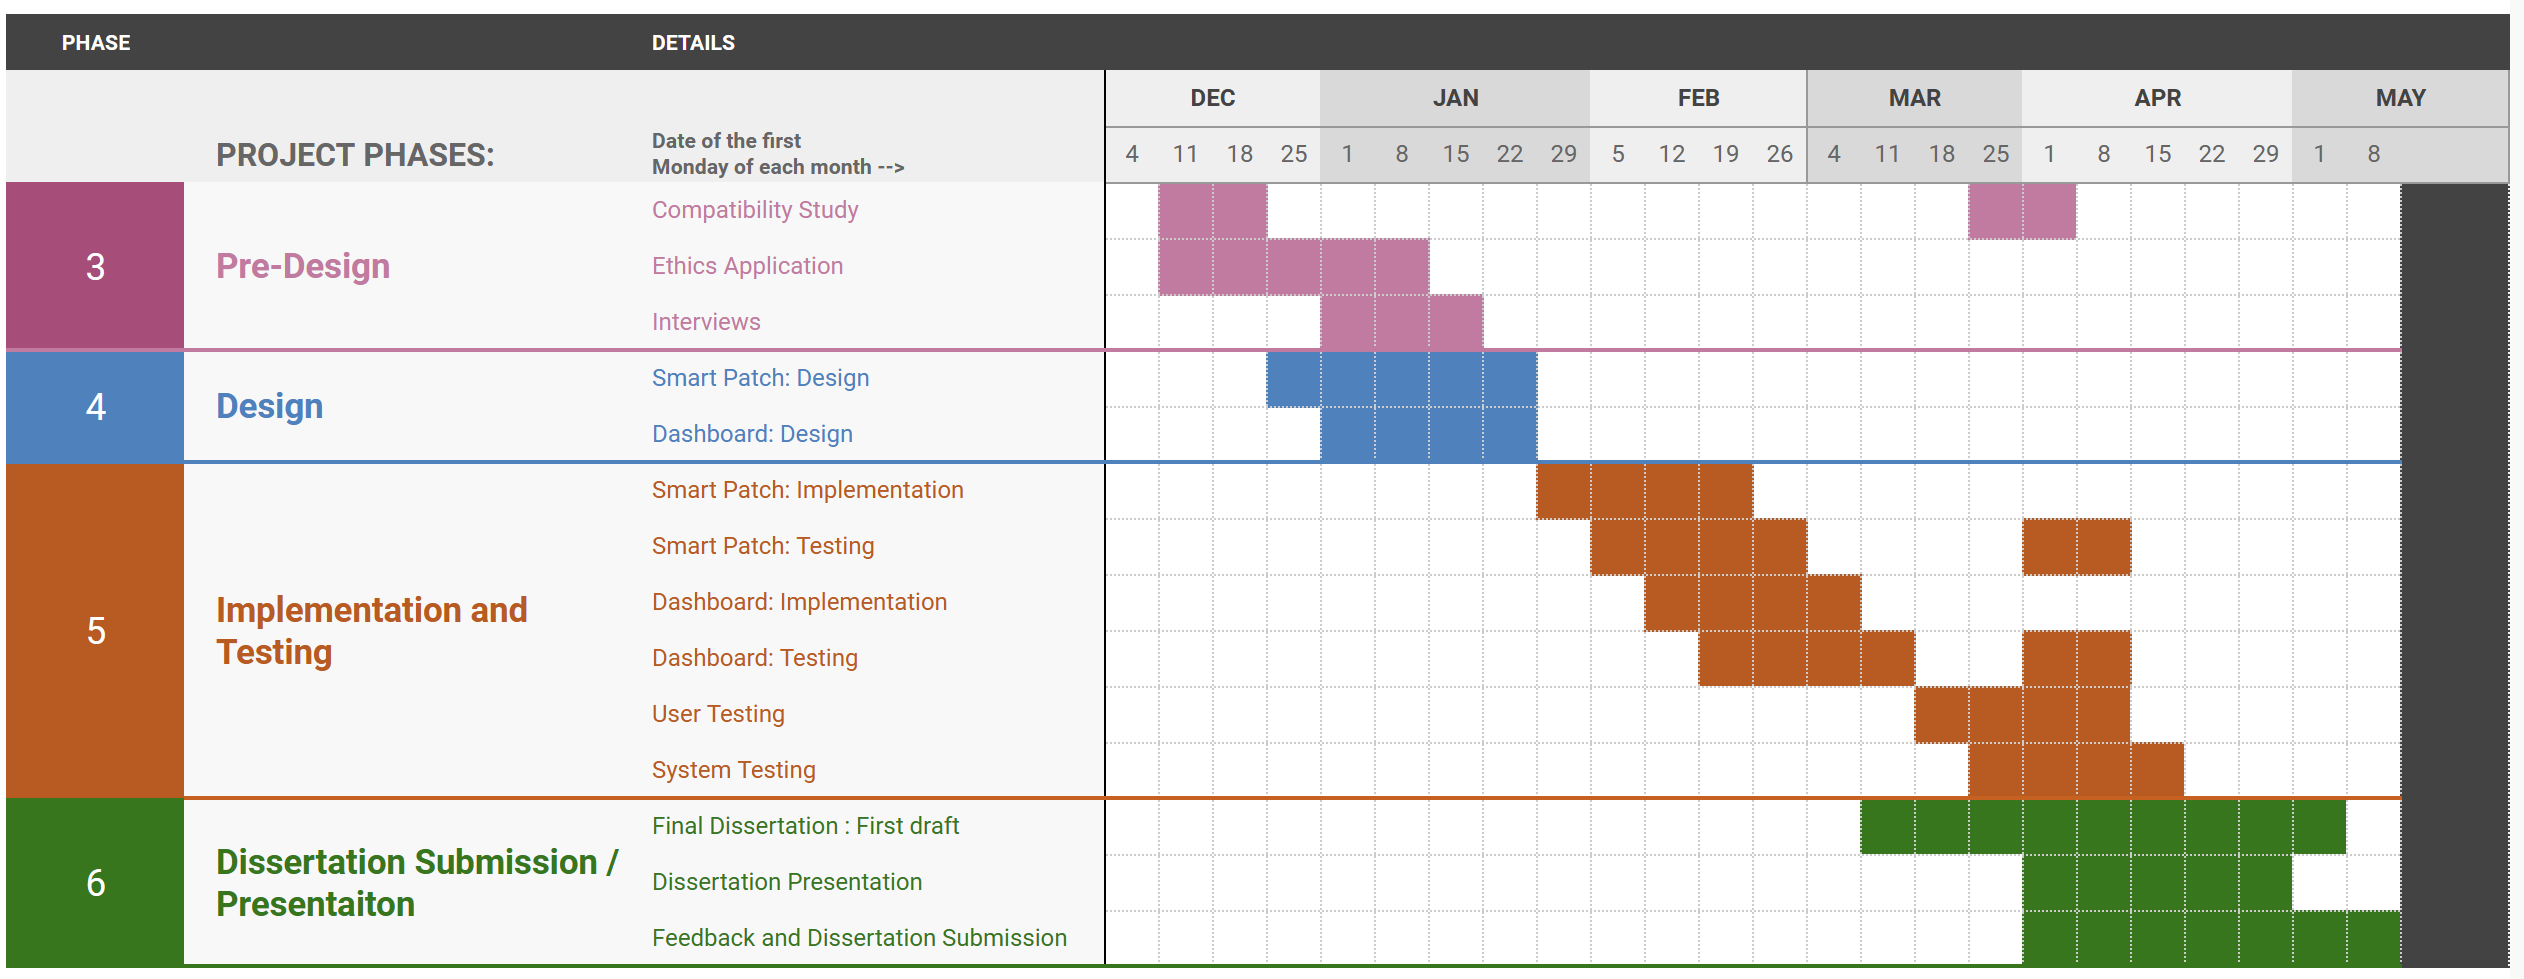
\includegraphics{images/gantt-chart.png}
%     \caption{Gantt Chart}
%     \label{fig:gantt-chart}
% \end{figure}

\section{Firmware}


The development of the Smart Patch firmware was characterized by a series of iterative improvements aimed at enhancing sensor accuracy, data handling, and user interaction. The project began with basic analog signal processing and gradually incorporated more sophisticated digital technologies and cloud-based integrations. Each iteration was driven by the dual goals of improving data reliability and enhancing user experience, while also adapting to technical challenges encountered along the way. \\

\noindent Initially, the firmware relied on analog signals to gather data from pulse sensor and LM-35 temperature sensor, which resulted in unstable and inaccurate readings. The shift to digital signal processing, and later to digital sensors like the DS18B20 for temperature sensing, marked significant advancements in data accuracy and stability. Integrating the system with cloud platforms such as Adafruit IO and external APIs like Twilio for SMS notifications brought about real-time data monitoring and interactive functionalities, further extending the capabilities of the Smart Patch. \\

\noindent The iterative development process was guided by continuous testing and feedback, which helped identify and rectify shortcomings in real-time. Challenges such as managing non-static IP addresses were addressed through architectural adjustments, notably the introduction of middleware to maintain connectivity and manageability. The final iterations focused on user management and data publishing control, allowing for more flexible and user-centric operation. \\

\noindent As of for the physical hardware - majorly the changes can be seen in from v1 to v6. Rest the hardware remained same. These can be seen in figures \ref{fig:v1-firmware} and \ref{fig:v6-firmware}.

\begin{figure}[h!]
    \centering
    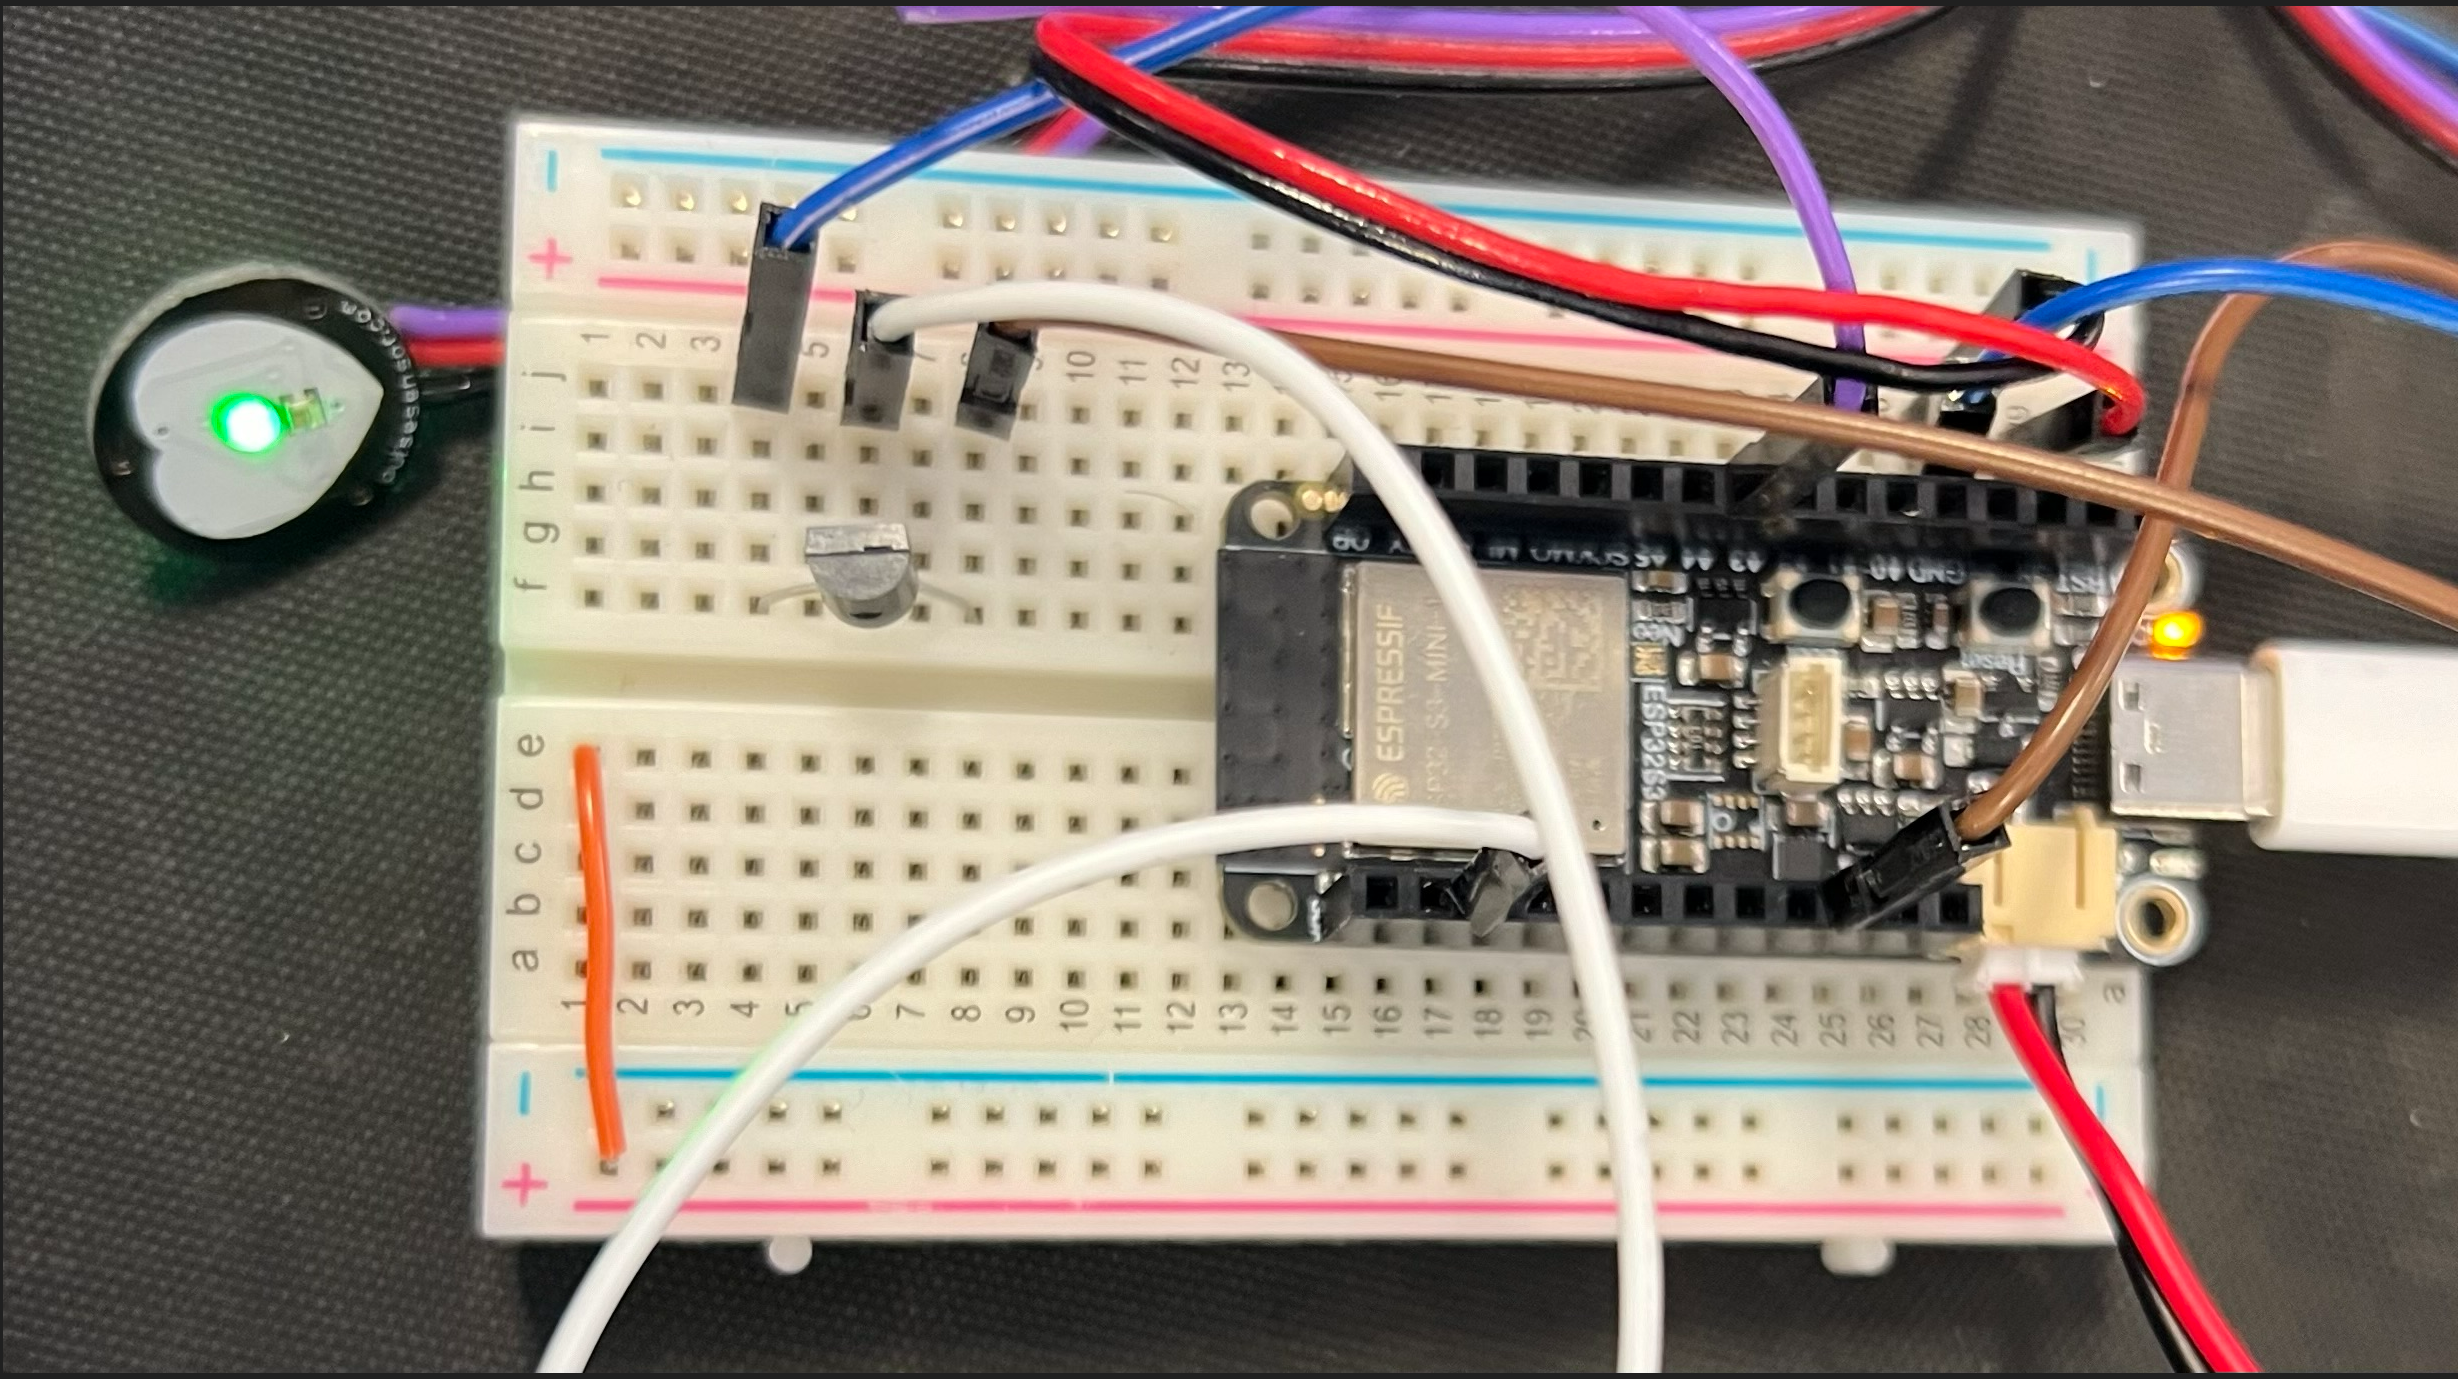
\includegraphics[width=1\linewidth]{images/v1-firmware.png}
    \caption{V1 Firmware}
    \label{fig:v1-firmware}
\end{figure}

\begin{figure}[h!]
    \centering
    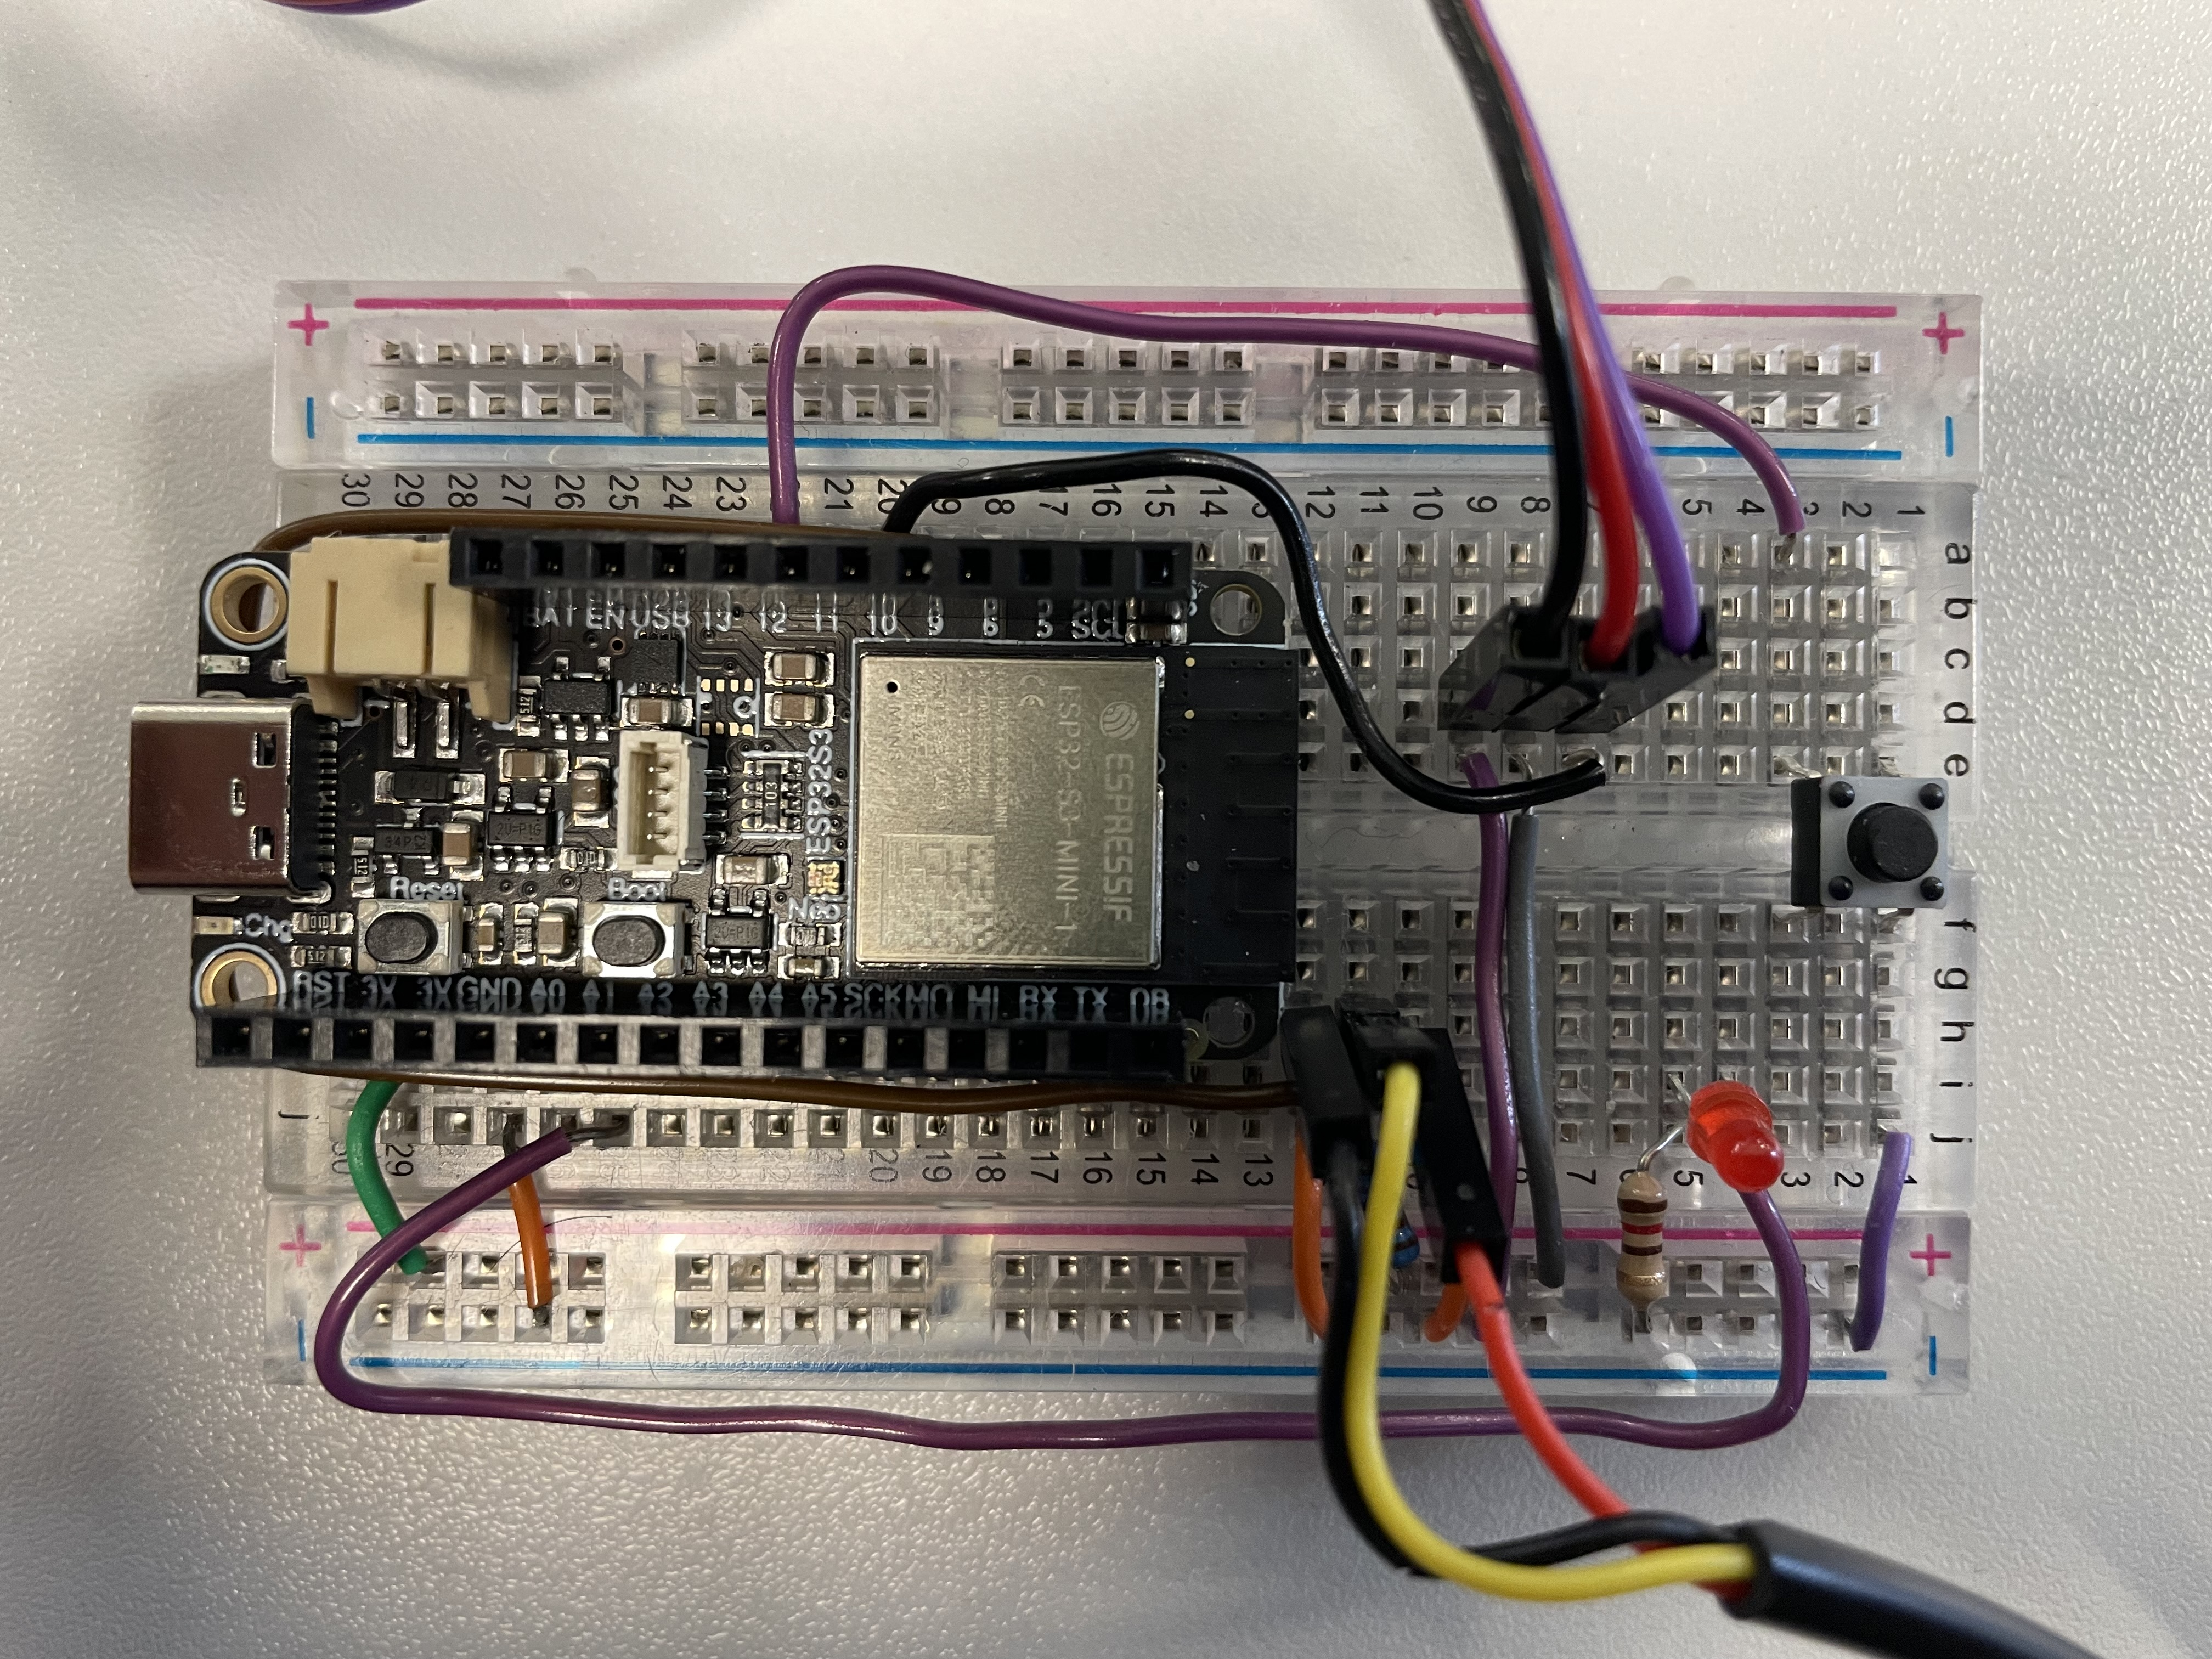
\includegraphics[width=1\linewidth]{images/v6-hardware.jpg}
    \caption{V6 Firmware}
    \label{fig:v6-firmware}
\end{figure}

\noindent Table \ref{tab:firmware_iterations} provides a summary of each iteration. \\

% \subsection{Iterative Development Journey}
% v1  - using analog signals and converting them into digital values to get data from PulseSensor and LM-35 sensor. The data received was neither accurate nor smooth.  \\
% v2 - For pulse sensor shifting from using analog signals to convert data to using libraries to get a direct digital value - LM-35 sensor's code remained same.this time to get more accurate data - collecting data of a minute removing bottom 10\% and top 10\% values to get smoother values. On testing, got to know that doing this still was not giving accurate values for temperature and as of Pulse sensor. So decided not to go forward with it. \\
% v3 - even then doing the both, was not getting a correct and smooth value from LM-35 sensor. Was advised to shift to a digital sensor - DS18B20.Tested things with it and got way more accurate and smooth data for temperature.  \\
% v4 - Connected to Wifi network, setup connected with Adafruit IO Dashboard by creating this esp as MQTT Client and publishing data on to 2 feeds - bpmFeed and temperatureFeed. These feeds were then subscribed by the dashboard. Tested whether the data is reflecting accurately and in real-time on the dashboard. Results were positive. \\
% v5 - Connected to Twilio API to send SMS when temperature crosses 35 degrees celcius. This was done statically to test the connection and how fast the SMS reaches to a person. Here the phone number is also static. Tests were positive but the messages were spamming because temperature doesn't fluctuate because if it stays above 35 it is going to be there for a while and everytime the condition is checked it will send an SMS. So added a condition that SMS will only be sent once every 30 mins. Tests were positive then.\\
% v6 - till now everything was in one file and it was becoming inefficient - divided things into separate files. Also added default values for name, phone number, and thresholds. We added a proper condition in the code comparing current values with the thresholds, only when it goes above or below the thresholds it sends an SMS. Added a switch and led to publish data only when the switch is turned on.  Created a temporary website on Flask to send data (name, phone number and thresholds) to the device - one major thing needed was the ip address and port number of the device to send/receive data. Tested to see if everything was working fine together. Results: Positive\\
% v7 - Data from the sensors were still a bit glitchy - so decided to implement Moving Average logic so that data never goes to extreme values. Gave it tolerance for each sensor so that beyond this the value should never go - if it goes skip the publishing logic. In addition to this, added an AnsyncWebServer to the device from where the temporary website could directly verify whether this device is active or not (connected to the network), to handle incoming data from the website about the user, and handle command of stop publishing when needed. Tests: Positive but a major challenge was that IP Addresses were not static. They change with changes in the network and then the data will never work out, and it would be hard for a not-so-tech-savvy person to create a static IP address for their network in the organization. So a different logic was needed to handle this - because it is not at all efficient. \\
% v8 - to handle the IP address issue, a middleware was introduced. So the idea behind it was that the middleware URL will be static and the device as soon as it gets connected to wifi will send a request to the middleware and share its IP Address which the middleware stores. Now in the user interface, organization admins don't have to know the ever-changing IP Addresses and change it every time - now they just need to remember the device's nickname and passkey which would never change. Along with this, another change in logic was made that the device should be easily switched between different users and when no users are assigned to the device, it should just not publish anything. Using that, streamlined the process by making it more about the user using it rather than about the device and making sure to get its credentials every time. To accomodate the middleware logic, had to change the code's asyncwebserver logic. Now the server's request were handled by /stop-publishing, /receive-user-details, /clear-user-details to receive data from the middleware. Along with this, it was thought that publishing data on the admin's website in addition to Adafruit IO dashboard would be quite useful to see real-time results on the same screen. This was tested well - and marked the end of Smart Patch's development. 


\begin{table}[h!]
\centering
\caption{Summary of Firmware Iterations}
\label{tab:firmware_iterations}
\begin{tabularx}{\textwidth}{|c|X|X|X|}
\hline
\textbf{Iteration} & \textbf{Description} & \textbf{Key Changes} & \textbf{Outcome} \\ \hline
v1 & Initial implementation using analog signals. & Utilized PulseSensor and LM-35 sensors with analog outputs. & Data was unstable and lacked accuracy. \\ \hline
v2 & Enhanced data handling by discarding outliers. & Implemented data smoothing by removing the top and bottom 10\% of readings; maintained analog LM-35 while shifting PulseSensor to digital. & Improved pulse data slightly; temperature readings remained unreliable. \\ \hline
v3 & Switch to digital temperature sensor. & Replaced LM-35 with DS18B20 for temperature measurements. & Achieved highly accurate and stable temperature data. \\ \hline
v4 & Integration with cloud and real-time data dashboard. & Connected to Wi-Fi; established MQTT client for Adafruit IO dashboard. & Successfully reflected real-time data on the dashboard. \\ \hline
v5 & Added SMS notifications for temperature alerts. & Integrated Twilio API to send SMS alerts when temperature exceeds 35°C; included rate-limiting. & Reduced spam with effective notification for critical temperature conditions. \\ \hline
v6 & Codebase optimization and user data management. & Refactored code into separate files; added web interface for user data input. & Enhanced efficiency and usability with better organization and user data integration. \\ \hline
v7 & Implemented data smoothing and reliability checks. & Introduced moving average logic for data smoothing and set tolerance thresholds for sensor data. & Further stabilized sensor data, but faced challenges with dynamic IP addresses. \\ \hline
v8 & Addressed connectivity issues; enhanced user management. & Implemented middleware for IP management; enhanced user-centric functionality and data privacy. & Resolved IP issues and improved system flexibility for user management and data handling. \\ \hline
\end{tabularx}
\end{table}


\noindent This section will discuss details as per the eight iteration.

\newpage
\subsection{Sensor Integration}

The integration of sensors into the firmware of the Smart Patch was a critical component of its development, enabling the device to capture real-time physiological data with high accuracy. This subsection details the integration processes for both the Pimoroni Pulse Sensor and the DS18B20 Temperature Sensor, as well as the implementation of a moving average filter to enhance sensor accuracy.

\subsubsection{Integration of Pimoroni Pulse Sensor}

The integration of the Pimoroni Pulse Sensor was implemented using the PulseSensorPlayground library to facilitate the capture of heartbeat signals. Configuration involved setting the input pin and threshold for beat detection. Below is the code used in the file \texttt{/esp/config.h}:

\begin{lstlisting}[language=C++, caption=Code for Pulse Sensor Integration]
// Pulse Sensor Setup
const int PulseWire = 10;
int Threshold = 550;
PulseSensorPlayground pulseSensor;

void setupSensors() {
    pulseSensor.analogInput(PulseWire);
    pulseSensor.setThreshold(Threshold);
    if (pulseSensor.begin()) {
        Serial.println("PulseSensor initialised!");
    }
}
\end{lstlisting}

This setup ensures that the pulse sensor is initialized correctly and ready to transmit pulse rate data to the main application.

\subsubsection{Integration of DS18B20 Temperature Sensor}

The DS18B20 Temperature Sensor, a digital sensor, was integrated using the OneWire and DallasTemperature libraries to allow for accurate temperature readings. The sensor was configured with the following initialization code (Listing~\ref{lst:temp-sensor} from the file \texttt{/esp/config.h}):

\begin{lstlisting}[language=C++, caption=Code for DS18B20 Integration, label=lst:temp-sensor]
// DS18b20 Sensor Setup
const int TempWire = 9;
OneWire oneWire(TempWire);
DallasTemperature tempSensors(&oneWire);

void setupSensors() {
    tempSensors.begin();
}
\end{lstlisting}

This configuration initializes the temperature sensor and prepares it to read temperatures in Celsius, which are then processed by the firmware.

\subsubsection{Sensor Accuracy - Moving Average}

To smooth out fluctuations in the data from both sensors and enhance accuracy, a moving average filter was implemented. This method averages the data points within a defined window to mitigate the effects of transient and noisy data. The following code (Listing~\ref{lst:moving-average} from the file \texttt{/esp/esp.ino}) illustrates the implementation of this moving average for both the pulse and temperature sensors:

\begin{lstlisting}[language=C++, caption=Implementation of Moving Average to increase sensor accuracy, label=lst:moving-average]
const int movingAverageWindowSize = 10;
float bpmSum = 0;
std::queue<int> bpmReadings;
float bpmMovingAverage = 0;
float tempSum = 0;
std::queue<float> tempReadings;
float tempMovingAverage = 0;

// Tolerance constants
const int BPM_TOLERANCE = 10; // Adjust based on testing and sensor accuracy
const float TEMP_TOLERANCE = 0.5; // Adjust based on testing and sensor accuracy

void updateMovingAverage(int bpm, float tempC) {
    // Update BPM moving average
    if (bpmReadings.size() >= movingAverageWindowSize) {
        bpmSum -= bpmReadings.front();
        bpmReadings.pop();
    }
    bpmSum += bpm;
    bpmReadings.push(bpm);
    bpmMovingAverage = bpmSum / bpmReadings.size();

    // Update Temperature moving average
    if (tempReadings.size() >= movingAverageWindowSize) {
        tempSum -= tempReadings.front();
        tempReadings.pop();
    }
    tempSum += tempC;
    tempReadings.push(tempC);
    tempMovingAverage = tempSum / tempReadings.size();
}
\end{lstlisting}

\noindent Through this implementation, both pulse and temperature readings are consistently averaged out, providing more reliable data to the system for further processing and decision-making.




\subsection{MQTT and Adafruit IO Integration}

The integration of MQTT protocol with Adafruit IO provides a robust solution for remote data monitoring and device management in the Smart Patch system. MQTT (Message Queuing Telemetry Transport) is a lightweight messaging protocol ideal for IoT applications due to its minimal bandwidth usage and effective data transmission even in unreliable networks.

\subsubsection{Configuration and Initialization}

The integration involves setting up an MQTT client with Adafruit IO as the broker. This setup utilizes the Adafruit MQTT library to establish a connection and publish data to specific feeds configured in the Adafruit IO dashboard. Below is the primary configuration used to initialize the MQTT client and data feeds:

\begin{lstlisting}[language=C++, caption={MQTT and Adafruit IO Client Configuration}]
#include "Adafruit_MQTT.h"
#include "Adafruit_MQTT_Client.h"

#define AIO_SERVER "io.adafruit.com"
#define AIO_SERVERPORT 1883
#define AIO_USERNAME "your_username"
#define AIO_KEY "your_aio_key"

// Setup the MQTT client class
Adafruit_MQTT_Client mqtt(&espClient, AIO_SERVER, AIO_SERVERPORT, AIO_USERNAME, AIO_KEY);
Adafruit_MQTT_Publish bpmFeed = Adafruit_MQTT_Publish(&mqtt, AIO_USERNAME "/feeds/BPM");
Adafruit_MQTT_Publish temperatureFeed = Adafruit_MQTT_Publish(&mqtt, AIO_USERNAME "/feeds/Temperature");
\end{lstlisting}

In this setup, the MQTT client is configured with server details and user credentials. Feeds for BPM and temperature data are defined using the username and a specific endpoint path that corresponds to each data type.


\noindent These code snippets and explanations outline the critical aspects of the MQTT and Adafruit IO integration within the Smart Patch system, demonstrating the implementation of network communication protocols to enhance IoT capabilities.

On the Adafruit IO D- the health-data dashboard looks like:

-- ADD IMAGE OF THE DASHBOARD


\subsection{Twilio Integration}

Twilio's cloud communication platform was integrated into the Smart Patch system to enable SMS notifications based on specific health data thresholds. This feature is particularly critical for immediate user notification in case of emergency health conditions. \\

\noindent The integration requires setting up authentication with Twilio's API using the account credentials and a messaging service SID, which are defined as constants. These credentials allow the device to authenticate with Twilio's servers securely and send SMS messages through the API.

\subsubsection{Sending SMS}

The function `sendSMS` constructs the request to send an SMS using HTTP POST. It constructs the URL and body dynamically using string streams and sends the request using the ESP32's HTTPClient library.

\begin{lstlisting}[language=C++, caption={Function to Send SMS via Twilio}]
bool sendSMS(const char *body) {
    std::stringstream url, urlEncodedBody;
    url << "https://api.twilio.com/2010-04-01/Accounts/" << accountNr << "/Messages";
    urlEncodedBody << "MessagingServiceSid=" << messagingServiceSid << "&To=" << to.c_str() << "&Body=" << body;

    HTTPClient http;
    http.begin(url.str().c_str());
    http.addHeader("Content-Type", "application/x-www-form-urlencoded");
    http.setAuthorization(accountNr, twilioPassword);
    int httpCode = http.POST(urlEncodedBody.str().c_str());

    http.end();
    return httpCode == 201;  // HTTP 201 indicates Created
}
\end{lstlisting}

\subsubsection{Threshold Alerts and SMS Notification Timing}

The system sends an SMS when temperature or BPM readings cross predefined thresholds. An important feature is the timing control, ensuring SMS alerts are sent no more than once every 30 minutes, regardless of sensor reading fluctuations.

\begin{lstlisting}[language=C++, caption={Conditional SMS Notifications Based on Thresholds}]
if (tempC > temp_upper_threshold || tempC < temp_lower_threshold || (bpm > bpm_upper_threshold && bpm > 0) || (bpm < bpm_lower_threshold && bpm > 0)) {
    unsigned long currentMillis = millis();  // Get current time in milliseconds
    // Check if at least 30 minutes have passed since the last SMS
    if (currentMillis - lastSMSTime >= 1800000) {
        char smsString[240]; 
        sprintf(smsString, "%s's Health Alert: Body Temperature has crossed %.2f°C and current BPM is %d.", name, tempC, bpm);
        if (sendSMS(smsString)) {
            lastSMSTime = currentMillis;  // Update the last SMS timestamp
            Serial.println("SMS sent successfully");
        } else {
            Serial.println("Failed to send SMS");
        }
    }
}
\end{lstlisting}

These segments of code highlight how the Twilio API is utilized for real-time health monitoring and alerting via SMS, enhancing the Smart Patch's capability to respond to critical health events efficiently.









\section{Middleware}
The Middleware component of the VitalMonitor system plays a crucial role as the intermediary layer that facilitates data communication and integration between the Smart Patch, the Dashboard, and the cloud-based database. Developed using the Flask framework, this Middleware is pivotal in managing the data flow within the system, ensuring that interactions are seamless and efficient.

\subsection{Connection with Google Cloud}
Key configurations of the middleware included establishing a connection to a Google Cloud MySQL instance via Unix sockets, ensuring secure and reliable database interactions. The use of environment variables (.env file) for sensitive information like database credentials was implemented.

\begin{lstlisting}[language=python, caption={Connection to Google Cloud MySQL using unix socket} label={lst:unix-socket}]
def connect_unix_socket() -> sqlalchemy.engine.base.Engine:
    """Initializes a Unix socket connection pool for a Cloud SQL instance of MySQL."""

    db_user = os.environ["DB_USER"]  # e.g. 'my-database-user'
    db_pass = os.environ["DB_PASS"]  # e.g. 'my-database-password'
    db_name = os.environ["DB_NAME"]  # e.g. 'my-database'
    unix_socket_path = os.environ[
        "INSTANCE_UNIX_SOCKET"
    ]  # e.g. '/cloudsql/project:region:instance'

    pool = sqlalchemy.create_engine(
        # Equivalent URL:
        # mysql+pymysql://<db_user>:<db_pass>@/<db_name>?unix_socket=<socket_path>/<cloud_sql_instance_name>
        sqlalchemy.engine.url.URL.create(
            drivername="mysql+pymysql",
            username=db_user,
            password=db_pass,
            database=db_name,
            host='34.147.167.209',
            query={
                "ssl_ca": "./permissions/server-ca.pem",
                "ssl_cert": "./permissions/client-cert.pem",
                "ssl_key": "./permissions/client-key.pem",
                "ssl_verify_cert": "false"
            },
        ),
    )

    return pool
\end{lstlisting}


\subsection{Database Integration}
The Middleware's database schema was designed to support complex data structures, involving multiple tables such as \textit{Organizations}, \textit{Users}, \textit{Devices}, and \textit{DeviceData}, each serving distinct data storage and retrieval functionalities. SQLAlchemy ORM was utilized for database operations, simplifying CRUD operations and enhancing the maintainability of the code. Flask-Migrate was integrated for handling database migrations, which assists in evolving the database schema over time without losing data.


\subsubsection{Security and Performance}
Security in data handling is paramount, especially given the sensitive nature of the stored health data. The \textit{Organization} model employs the Flask-Bcrypt library for secure password handling:

\begin{lstlisting}[language=python, caption={Secure Password Handling in Organization Model}]
from flask_bcrypt import Bcrypt

bcrypt = Bcrypt()

class Organization(db.Model):
    __tablename__ = 'organizations'
    password_hash = db.Column(db.String(255), nullable=False)

    def set_password(self, password):
        self.password_hash = bcrypt.generate_password_hash(password).decode('utf-8')

    def check_password(self, password):
        return bcrypt.check_password_hash(self.password_hash, password)
\end{lstlisting}

The connection between the middleware and Google Cloud is more secure by using permission files (used in Listing \ref{lst:unix-socket}) which can only be generated once from the cloud. Without these permissions files, middleware won't get connected to the cloud.

\subsection{API Integration}

API endpoints were carefully crafted to support essential operations such as user and device registration, login processes, and data transmission between devices and the Dashboard. These endpoints handle data validation, session management, and error responses effectively, ensuring a seamless user experience and robust data handling.

\subsubsection{User and Organization Management}

The API endpoints for registering organizations and users are fundamental for setting up and securing access to the system. They ensure that only authorized entities can register and manage devices and users. Below are examples of these key functionalities:

\begin{lstlisting}[language=python, caption={API Endpoint for Organization Registration}]
@app.route('/register', methods=['POST'])
def register_organization():
    data = request.json
    name = data.get('name')
    password = data.get('password')
    if not name or not password:
        return jsonify({"error": "Name and password are required"}), 400
    if Organization.query.filter_by(name=name).first():
        return jsonify({"error": "Organization already exists"}), 400
    new_organization = Organization(name=name)
    new_organization.set_password(password)
    db.session.add(new_organization)
    try:
        db.session.commit()
    except Exception as e:
        db.session.rollback()
        return jsonify({"error": str(e)}), 500
    return jsonify({"success": "Organization registered successfully", "organization_id": new_organization.id, "organization_name": name}), 201
\end{lstlisting}

\noindent This endpoint performs critical checks such as validation of input fields and checks against existing records, ensuring data integrity and preventing duplicates in the system.

\subsubsection{Device Management}

Device management is crucial for tracking and updating the status and configuration of devices connected to the system. The API allows for device addition, updates, and assignment to users or organizations, as shown in the following example:

\begin{lstlisting}[language=python, caption={API Endpoint for Adding or Updating a Device}]
@app.route('/add-new-device', methods=['POST'])
def add_or_update_device():
    data = request.json
    mac_address = data.get('mac_address')
    ip_address = data.get('ip_address')
    passkey = data.get('passkey')
    nickname = data.get('nickname')
    device = Device.query.filter_by(mac_address=mac_address).first()
    if device:
        device.ip_address = ip_address
    else:
        device = Device(mac_address=mac_address, ip_address=ip_address, nickname=nickname, passkey=passkey)
        db.session.add(device)
    try:
        db.session.commit()
        return jsonify({"success": "Device added or updated successfully", "device_id": device.id}), 201
    except Exception as e:
        db.session.rollback()
        return jsonify({"error": str(e)}), 500
\end{lstlisting}

\noindent This endpoint not only facilitates the registration of new devices but also handles updates to existing ones, demonstrating the dynamic nature of device management within the system.

\subsubsection{Real-Time Data Interaction}

For real-time interaction, APIs facilitate the immediate relay of data between the devices and the system. This includes sending updated configuration details to the devices or receiving real-time data for display on the dashboard.

\begin{lstlisting}[language=python, caption={API Endpoint for Real-Time Data Streaming}]
@app.route('/get-device-data/<int:device_id>', methods=['GET'])
def get_device_data(device_id):
    def generate():
        with app.app_context():
            while True:
                latest_data = DeviceData.query.filter_by(device_id=device_id).order_by(DeviceData.timestamp.desc()).first()
                yield f"data:{json.dumps({'bpm': latest_data.bpm, 'temperature': latest_data.temperature})}\n\n"
                time.sleep(5)  # Adjust as necessary for your application's needs
    return Response(generate(), content_type='text/event-stream', headers={'Cache-Control': 'no-cache'})
\end{lstlisting}

\noindent This streaming API is essential for maintaining a live dashboard that reflects the most current data from connected devices.

\noindent These API integrations are pivotal in ensuring that the Middleware efficiently handles all communications within the VitalMonitor system, thus supporting robust, scalable, and secure operations.


\section{Web Dashboard}
The implementation phase of the Web Dashboard for the VitalMonitor system was guided by a commitment to reliability, security, and enhancing user efficiency. Leveraging a streamlined technology stack composed of Flask, HTML, CSS, and JavaScript, the development went beyond merely meeting functional requirements. It also focused on delivering an engaging and effective user experience for organization administrators. Most of the development is very straightforward and didn't involve much complexities unlike for Smart Patch and Middleware. Some important implementations of certain components of the website are discussed below.

\subsection{Session Management using custom decorators}

As per the design discussed in the last chapter, Custom Decorators were used for session management. Custom Decorators are nothing but a function that adds functionality to another function or method without modifying its structure. This is particularly useful in web development for handling tasks like authentication and authorization. In this case provided in Listing \ref{Session Management}, \textit{@login\_required} decorator, it acts as a gatekeeper for routes that require user authentication. \\ 

When applied, such as before the \textit{add\_device\_page()} function, the \textit{login\_required} decorator checks whether the \textit{organization\_id} exists in the session. This \textit{organization\_id} is crucial as it signifies that the admin representing an organization is currently logged in. If the check fails (i.e., if \textit{organization\_id} is not found), it redirects the admin to the login page. This prevents unauthorized users or admins from accessing routes that are meant to be secured, thereby protecting sensitive actions like adding devices.

\begin{lstlisting}[language=python, caption=Custom Decorator - login\_required, label=Session Management]
def login_required(f):
    @wraps(f)
    def decorated_function(*args, **kwargs):
        if 'organization_id' not in session:
            return redirect(url_for('register_login_page'))
        return f(*args, **kwargs)
    return decorated_function

@app.route('/add-device-page')
    @login_required
    def add_device_page():
        organization_name = session.get('organization_name')
        return render_template('add_device.html', organization_name=organization_name)
\end{lstlisting}


\subsection{Real-time Data}

The real-time data fetching mechanism is used for user pages. Figure \ref{fig:user-page-real-time-fetching-code} demonstrated in the JavaScript code utilizes Server-Sent Events (SSE) to establish a continuous stream from a server to the web browser. Specifically, the function \textit{startLiveDataStream(deviceId)} initiates the connection using the EventSource API, which connects to a specified URL that corresponds to the device ID. Once connected, the server streams data in real-time, sending updates that are automatically received by the client-side JavaScript. Additionally, the function implements robust error handling and auto-reconnect features. If the connection fails or the page becomes invisible, the connection is closed, and attempts to reconnect are made automatically, ensuring continuous data delivery without manual refresh.

\begin{figure}[h!]
    \centering
    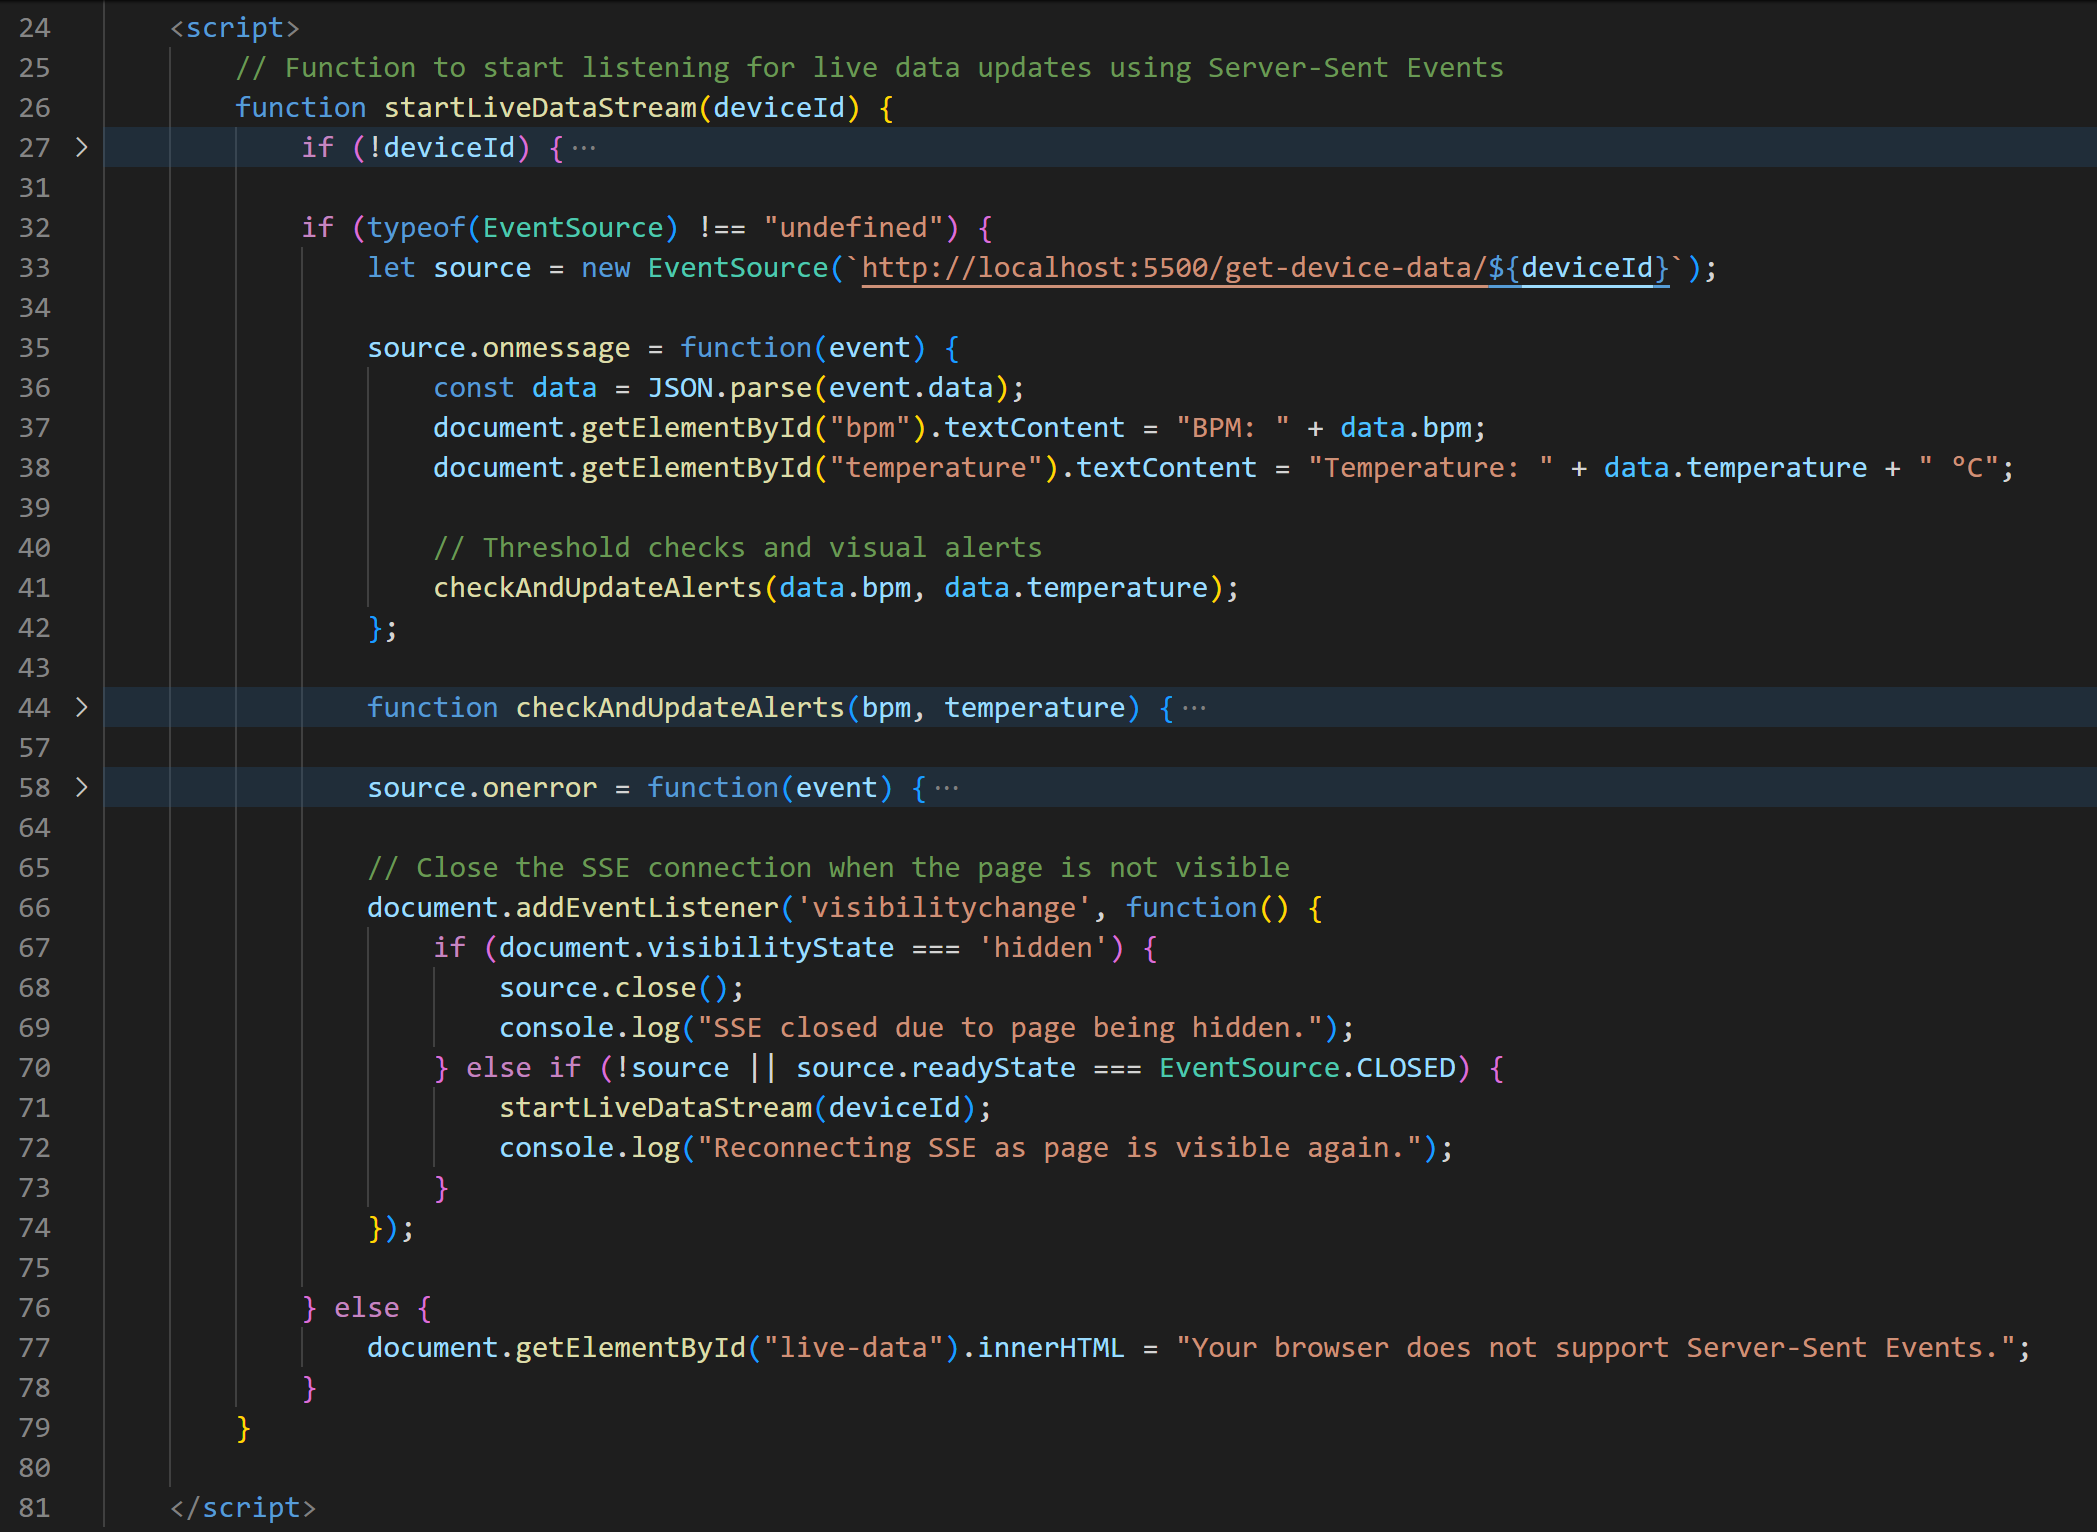
\includegraphics[width=1\linewidth]{images/user-page-real-time-fetching-code.png}
    \caption{Fetching User Health Data in real-time.}
    \label{fig:user-page-real-time-fetching-code}
\end{figure}

\subsection{User Interface and Interaction}
The design of the dashboard prioritizes ease of use and a minimalistic approach as seen in Figures \ref{fig:login-page} - \ref{fig:about-page}. Two major things that were taken care of while implementing the UI were:

\begin{itemize}

    \item \textbf{User Navigation:}
     The dashboard layout emphasizes navigational clarity, allowing admins to smoothly transition between viewing all users, managing individual profiles, and device settings without complex navigation steps.
    
    \item \textbf{Actionable Insights:}
     Interactive elements such as buttons and links are strategically placed to facilitate the easy completion of administrative tasks, such as adding or updating user information, managing devices, and monitoring health vitals.

\end{itemize}

\begin{figure}[h!]
    \centering
    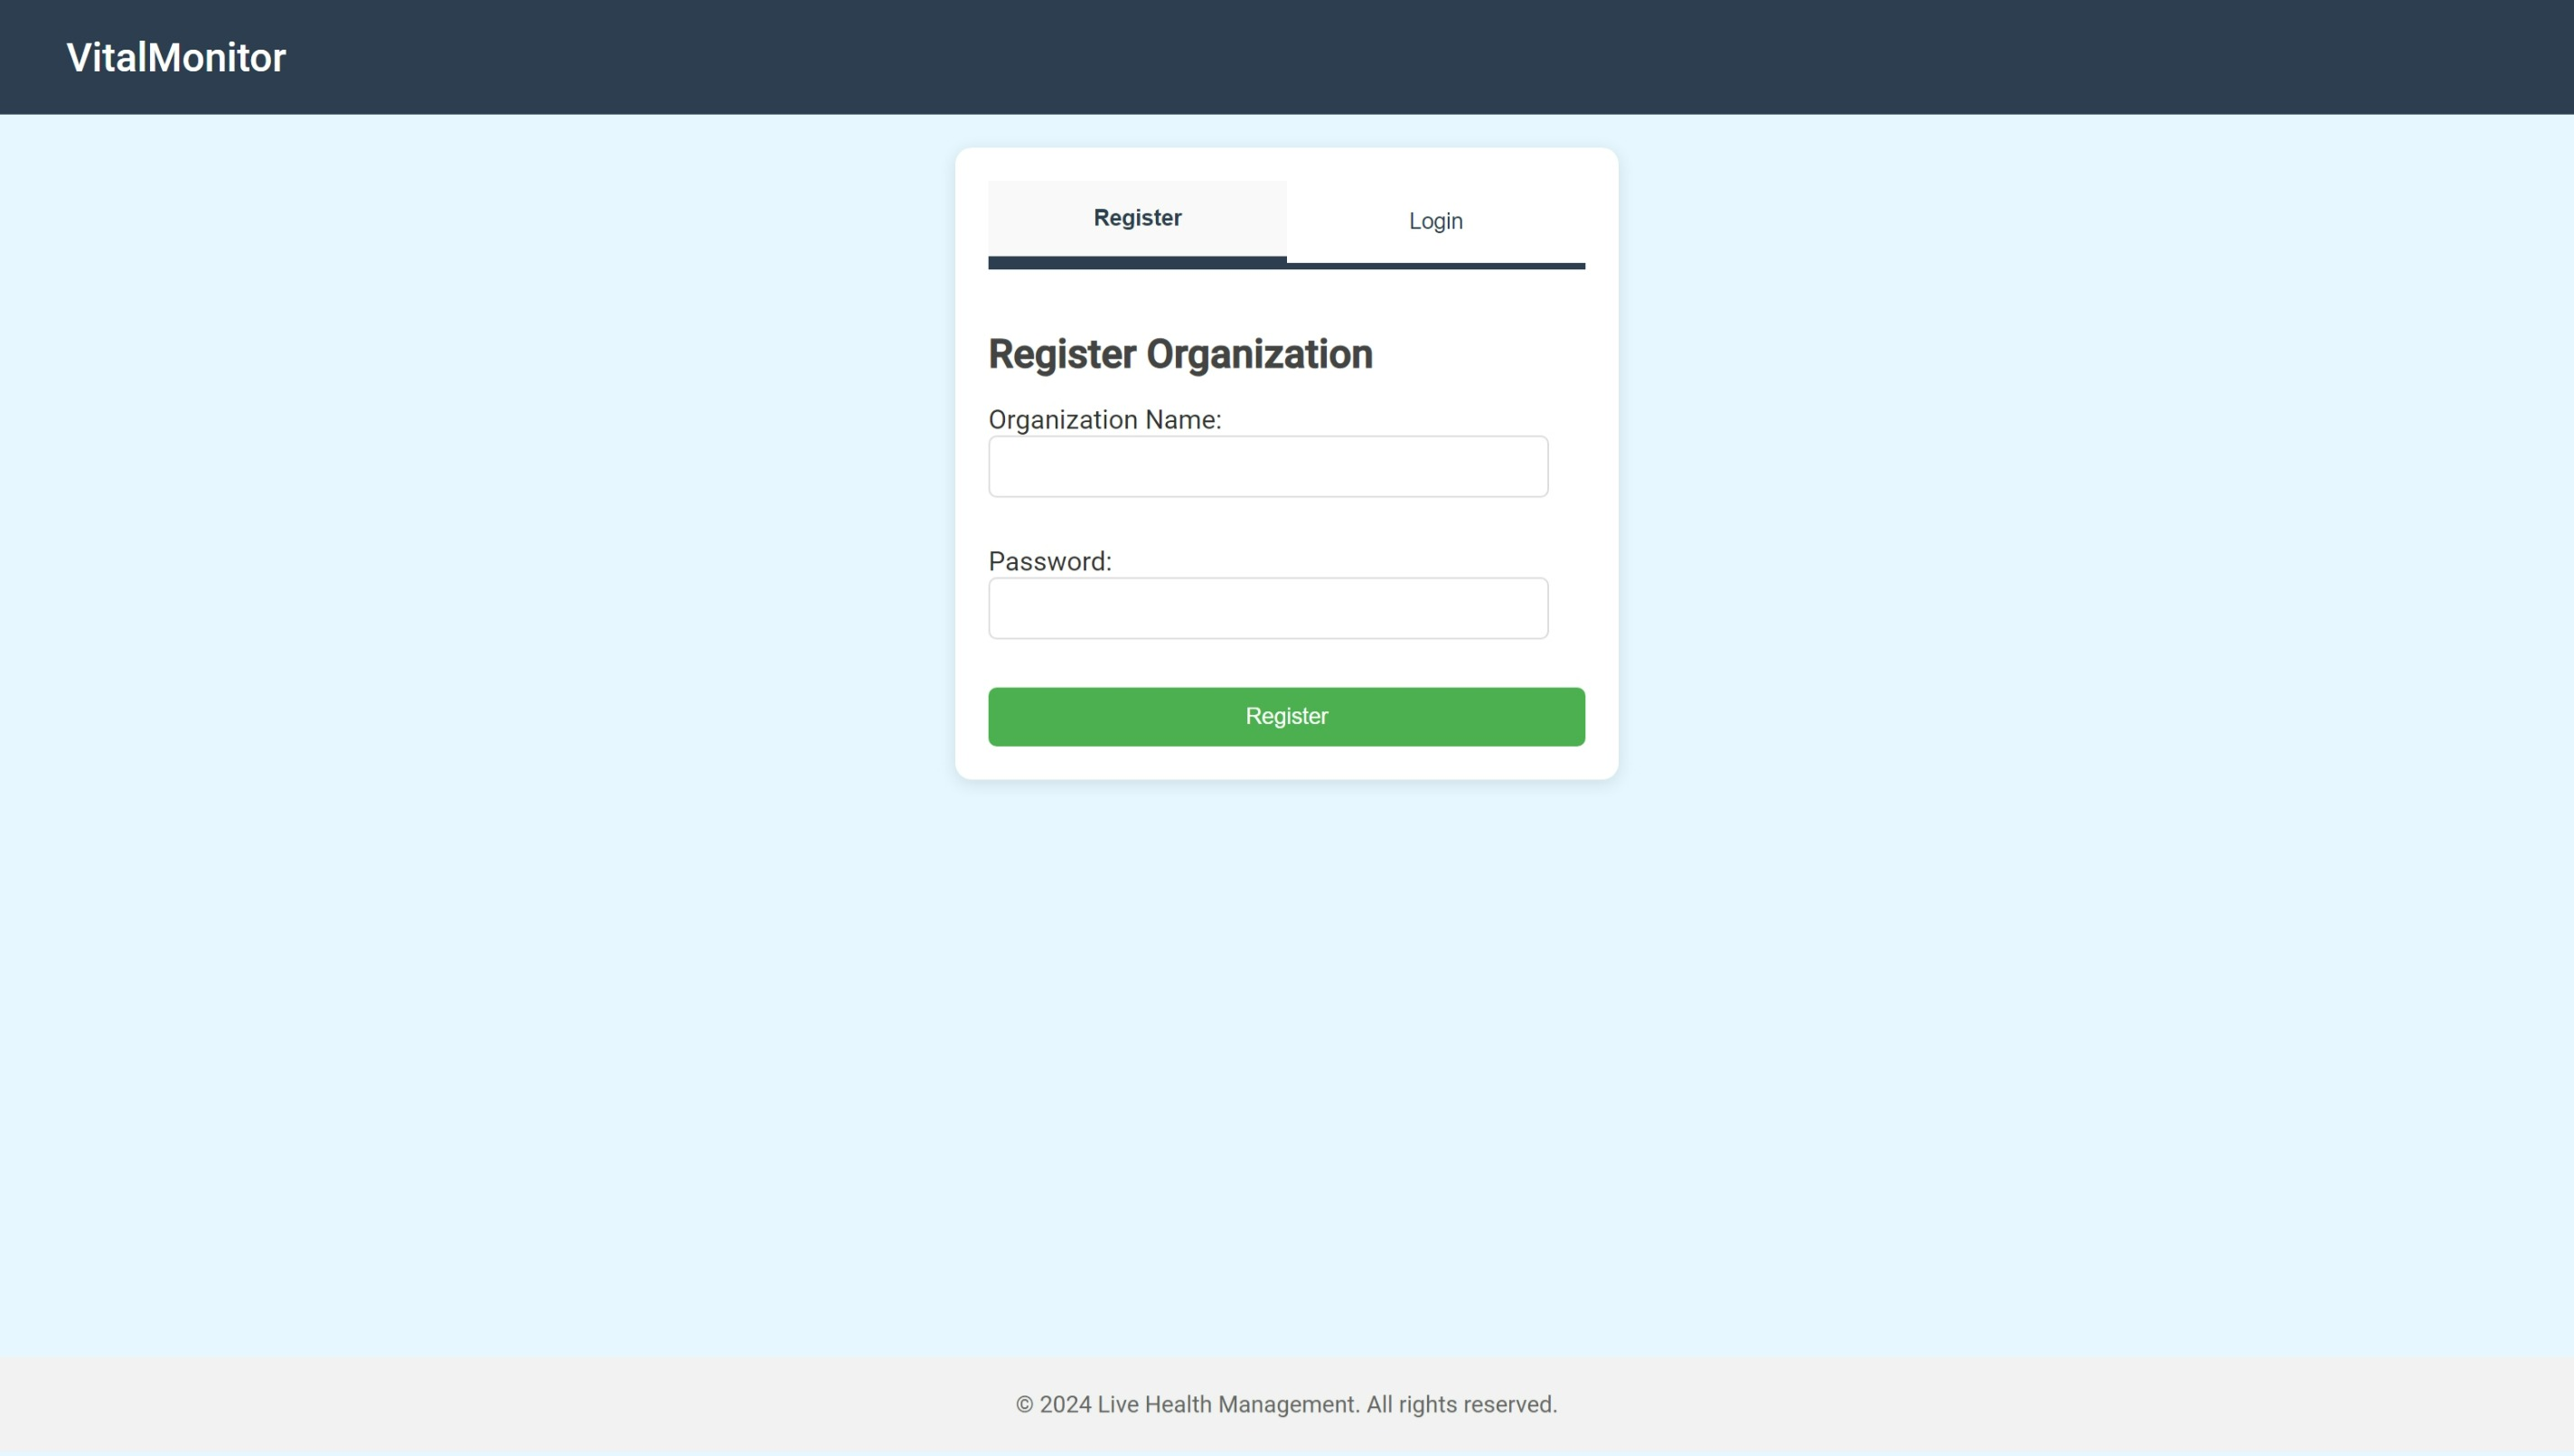
\includegraphics[width=1\linewidth]{images/dashboard-6.jpeg}
    \caption{Login and Register Page (landing page)}
    \label{fig:login-page}
\end{figure}

\begin{figure}[h!]
    \centering
    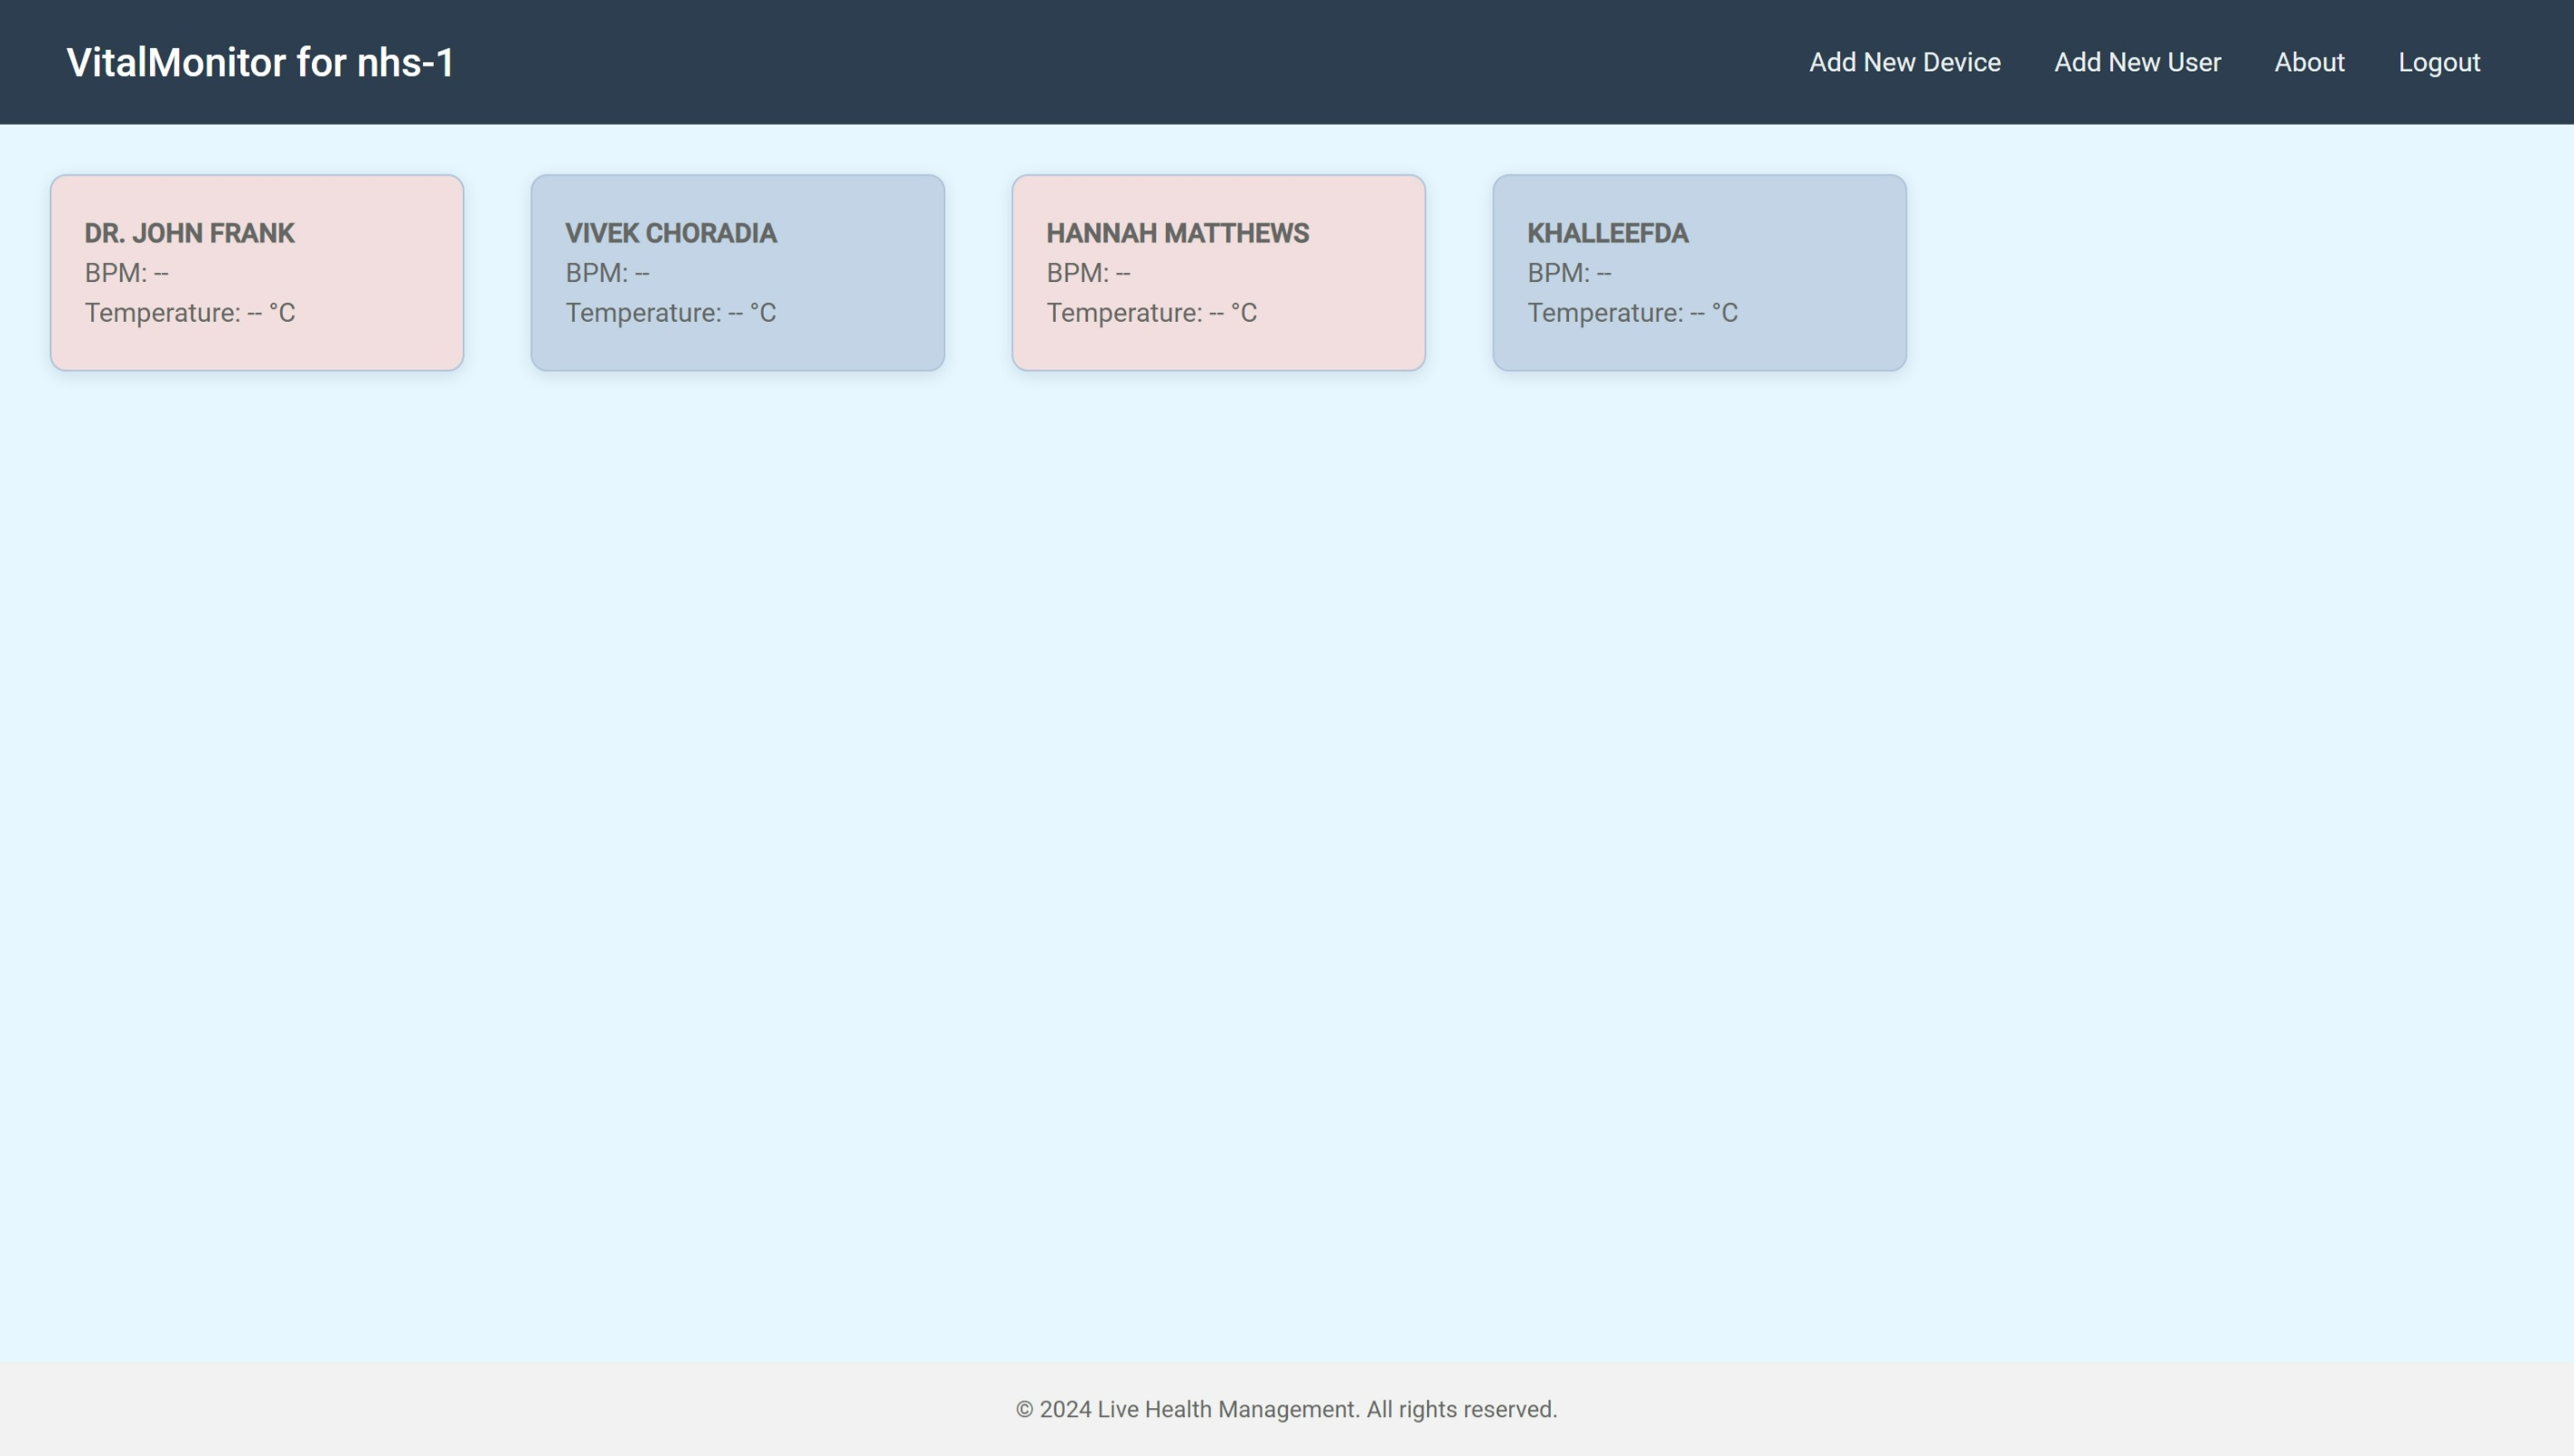
\includegraphics[width=1\linewidth]{images/dashboard-5.jpeg}
    \caption{Home Page}
    \label{fig:home-page}
\end{figure}

\begin{figure}[h!]
    \centering
    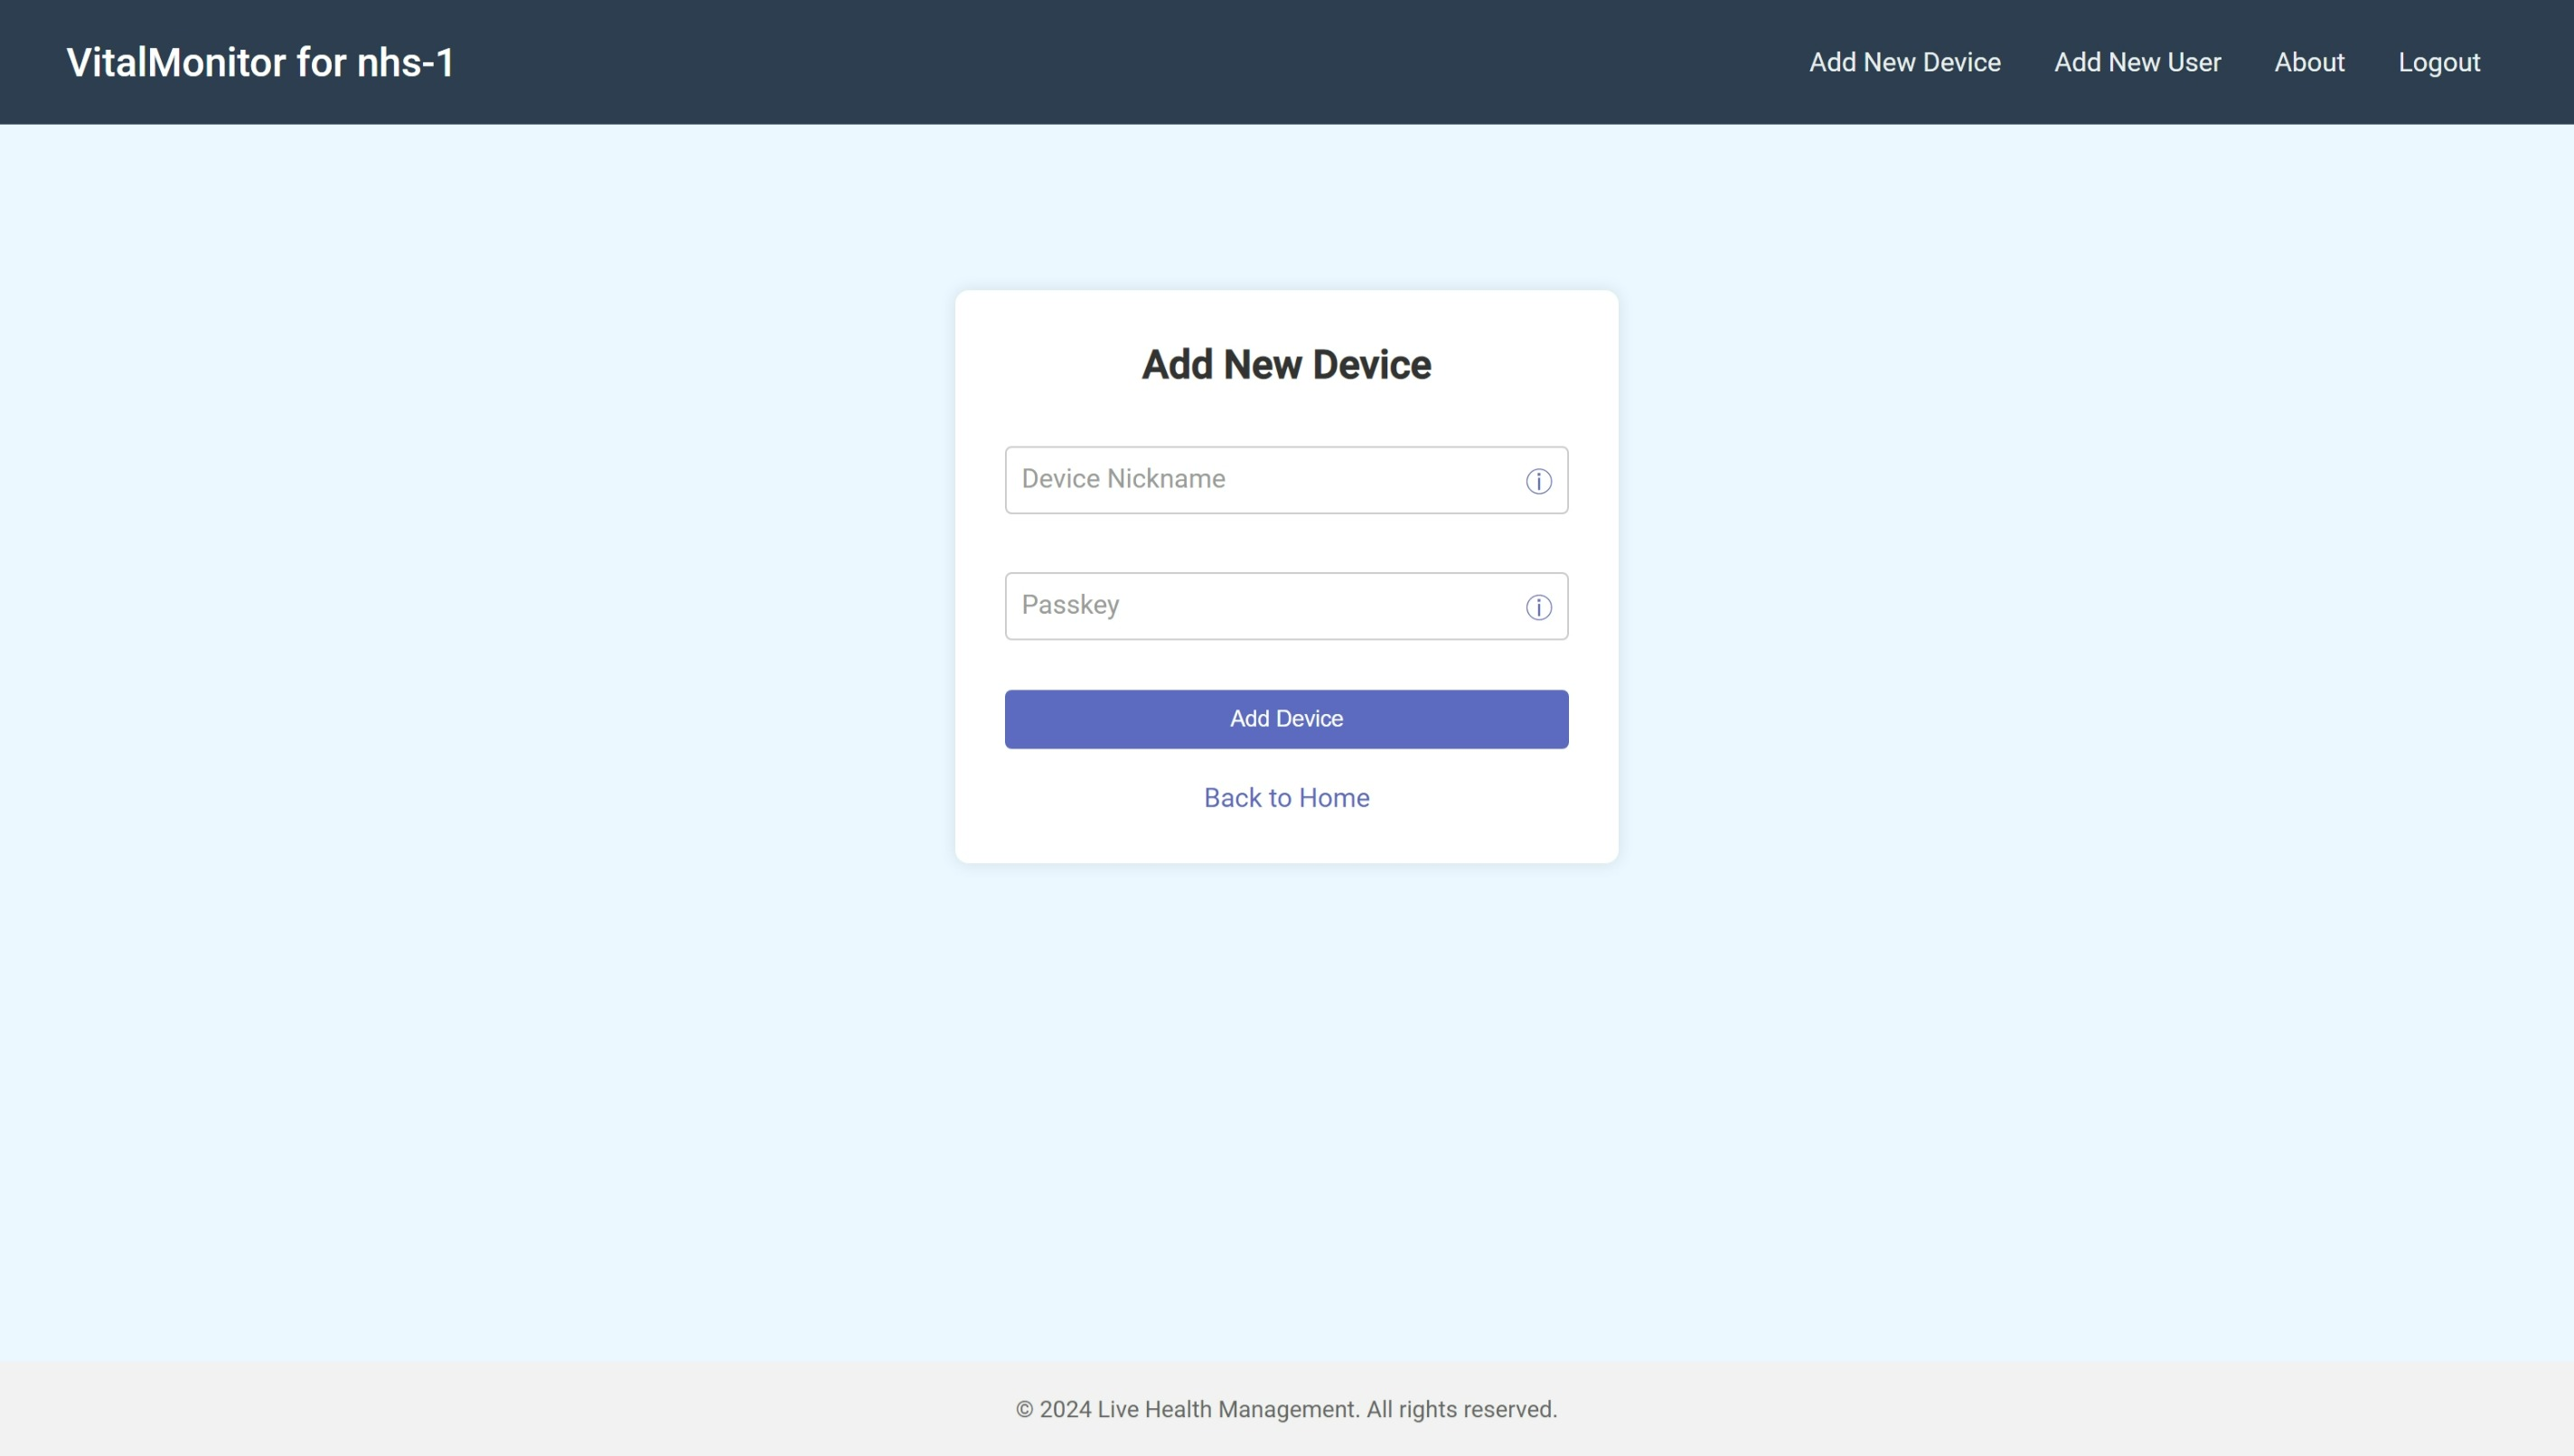
\includegraphics[width=1\linewidth]{images/dashboard-4.jpeg}
    \caption{Add New Device Page}
    \label{fig:device-page}
\end{figure}

\begin{figure}[h!]
    \centering
    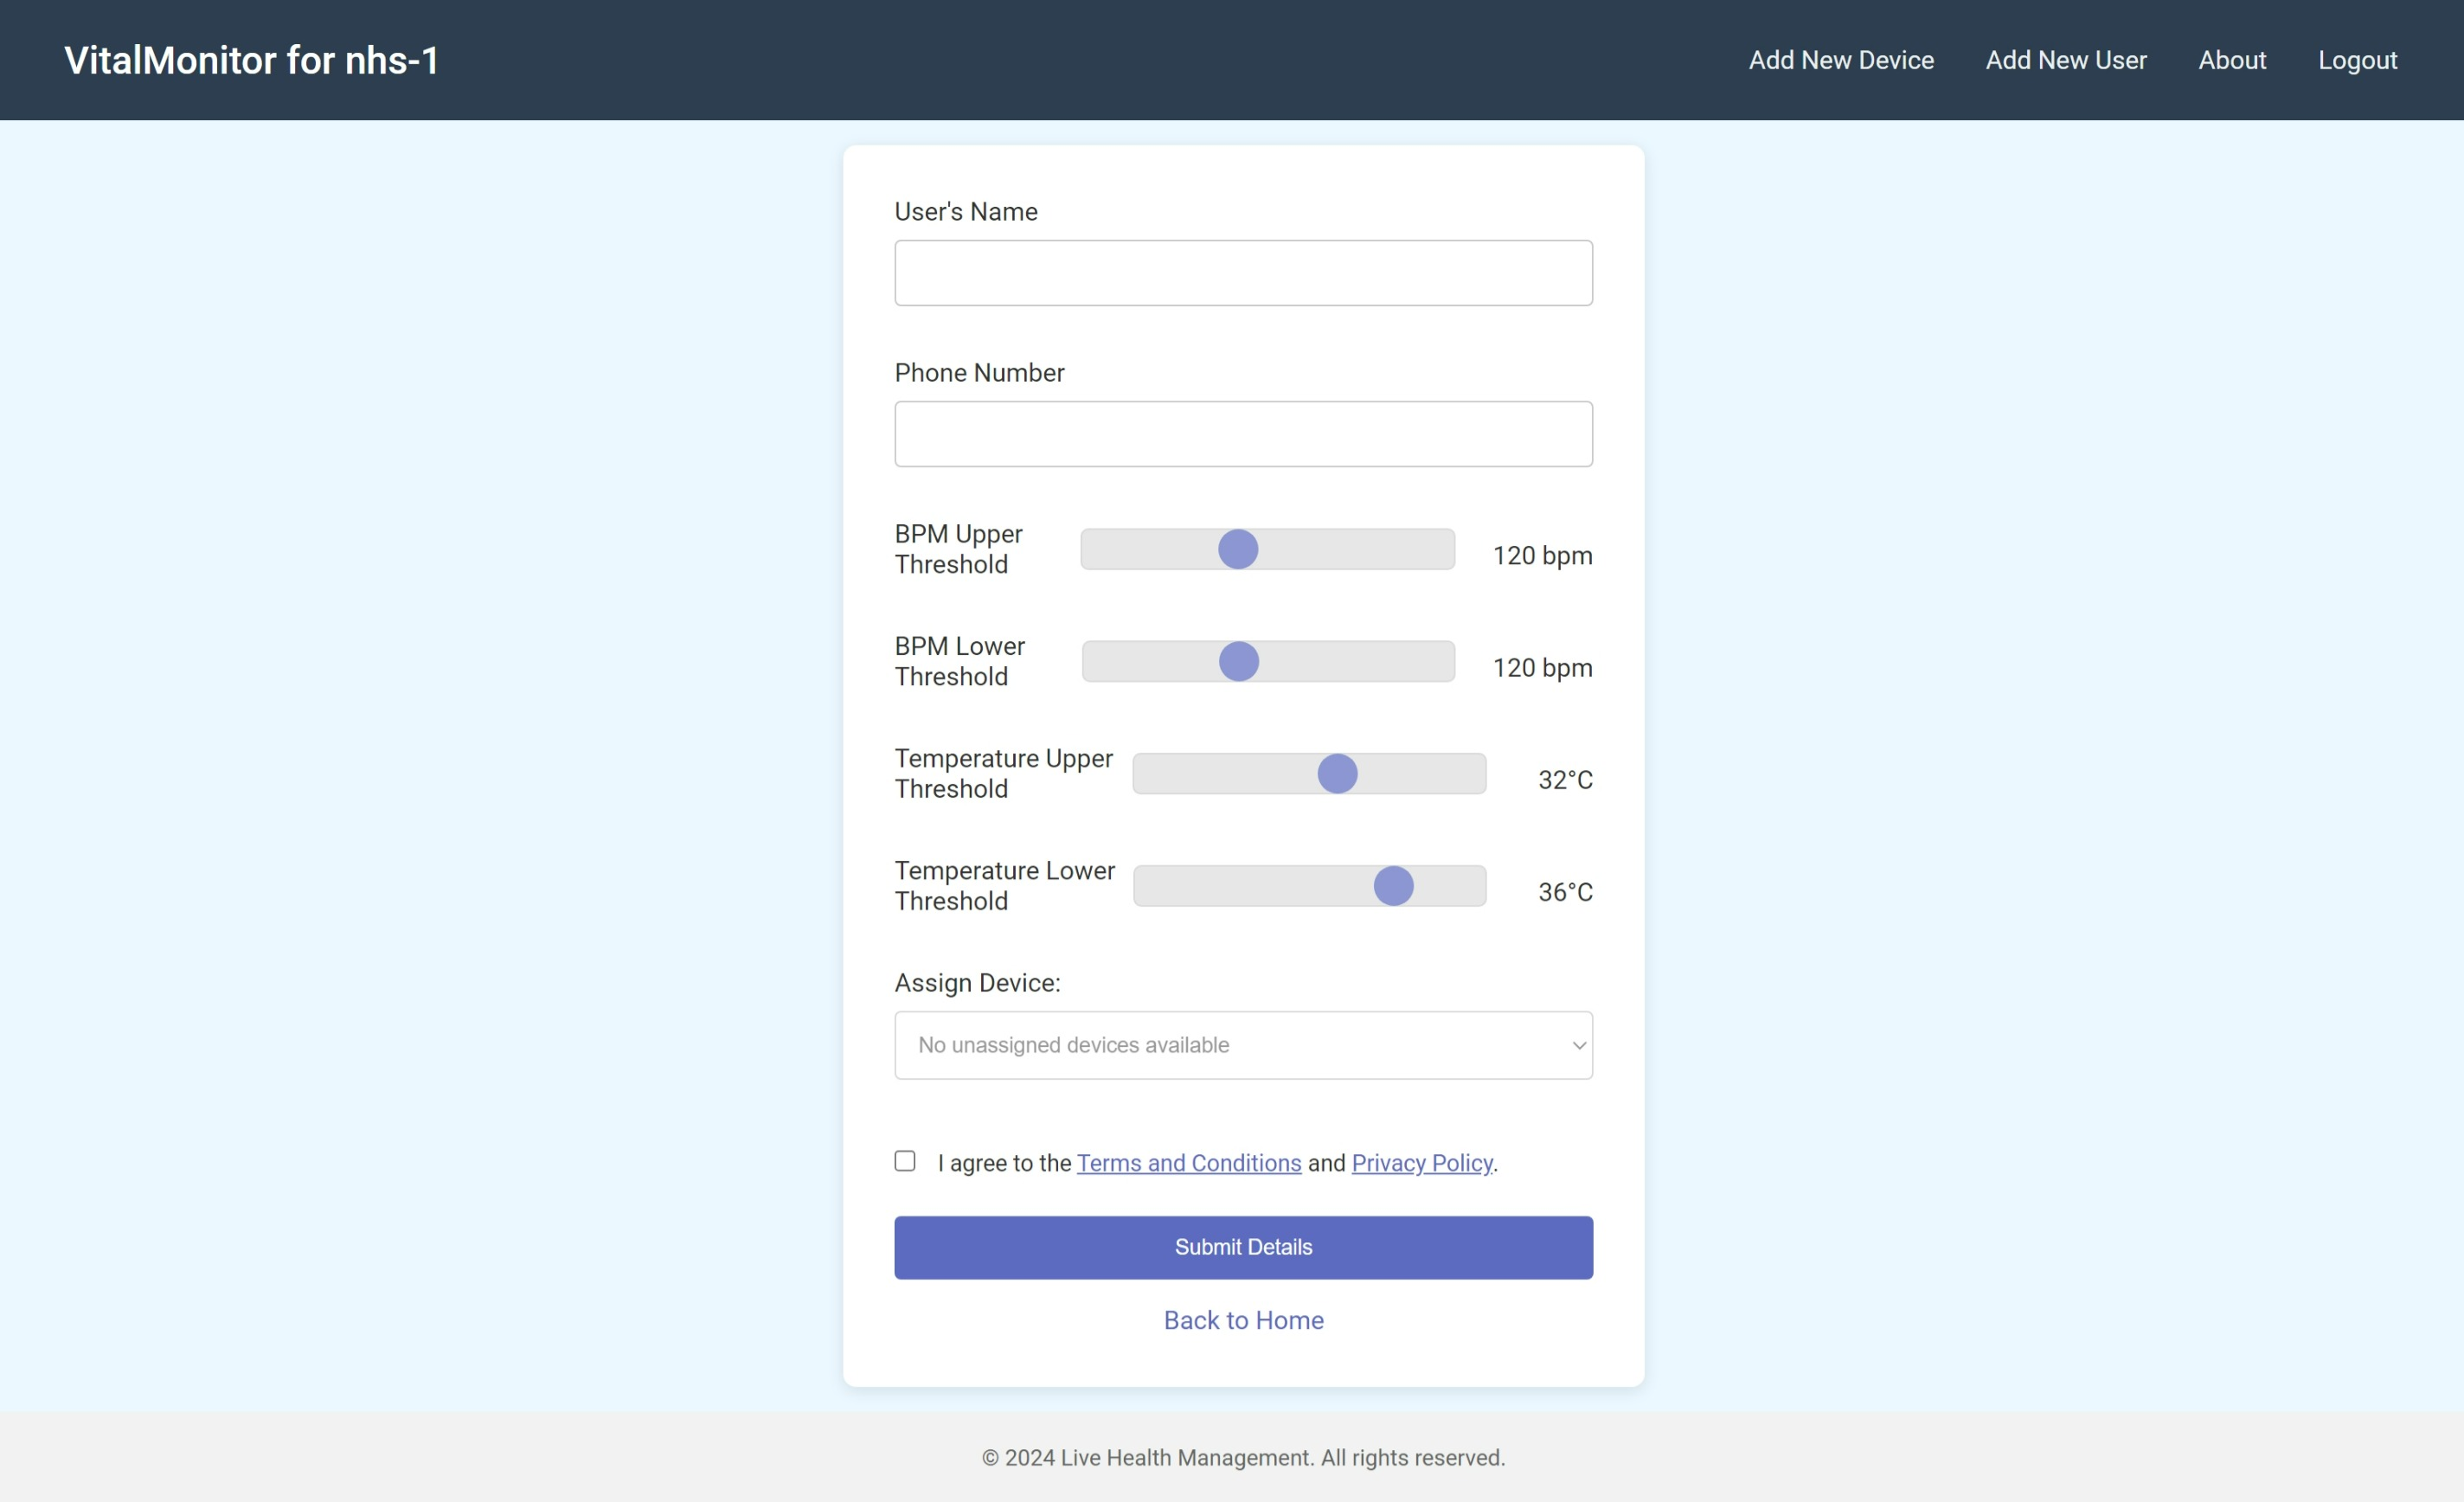
\includegraphics[width=1\linewidth]{images/dashboard-3.jpeg}
    \caption{Add New User Page}
    \label{fig:new-user-page}
\end{figure}

\begin{figure}[h!]
    \centering
    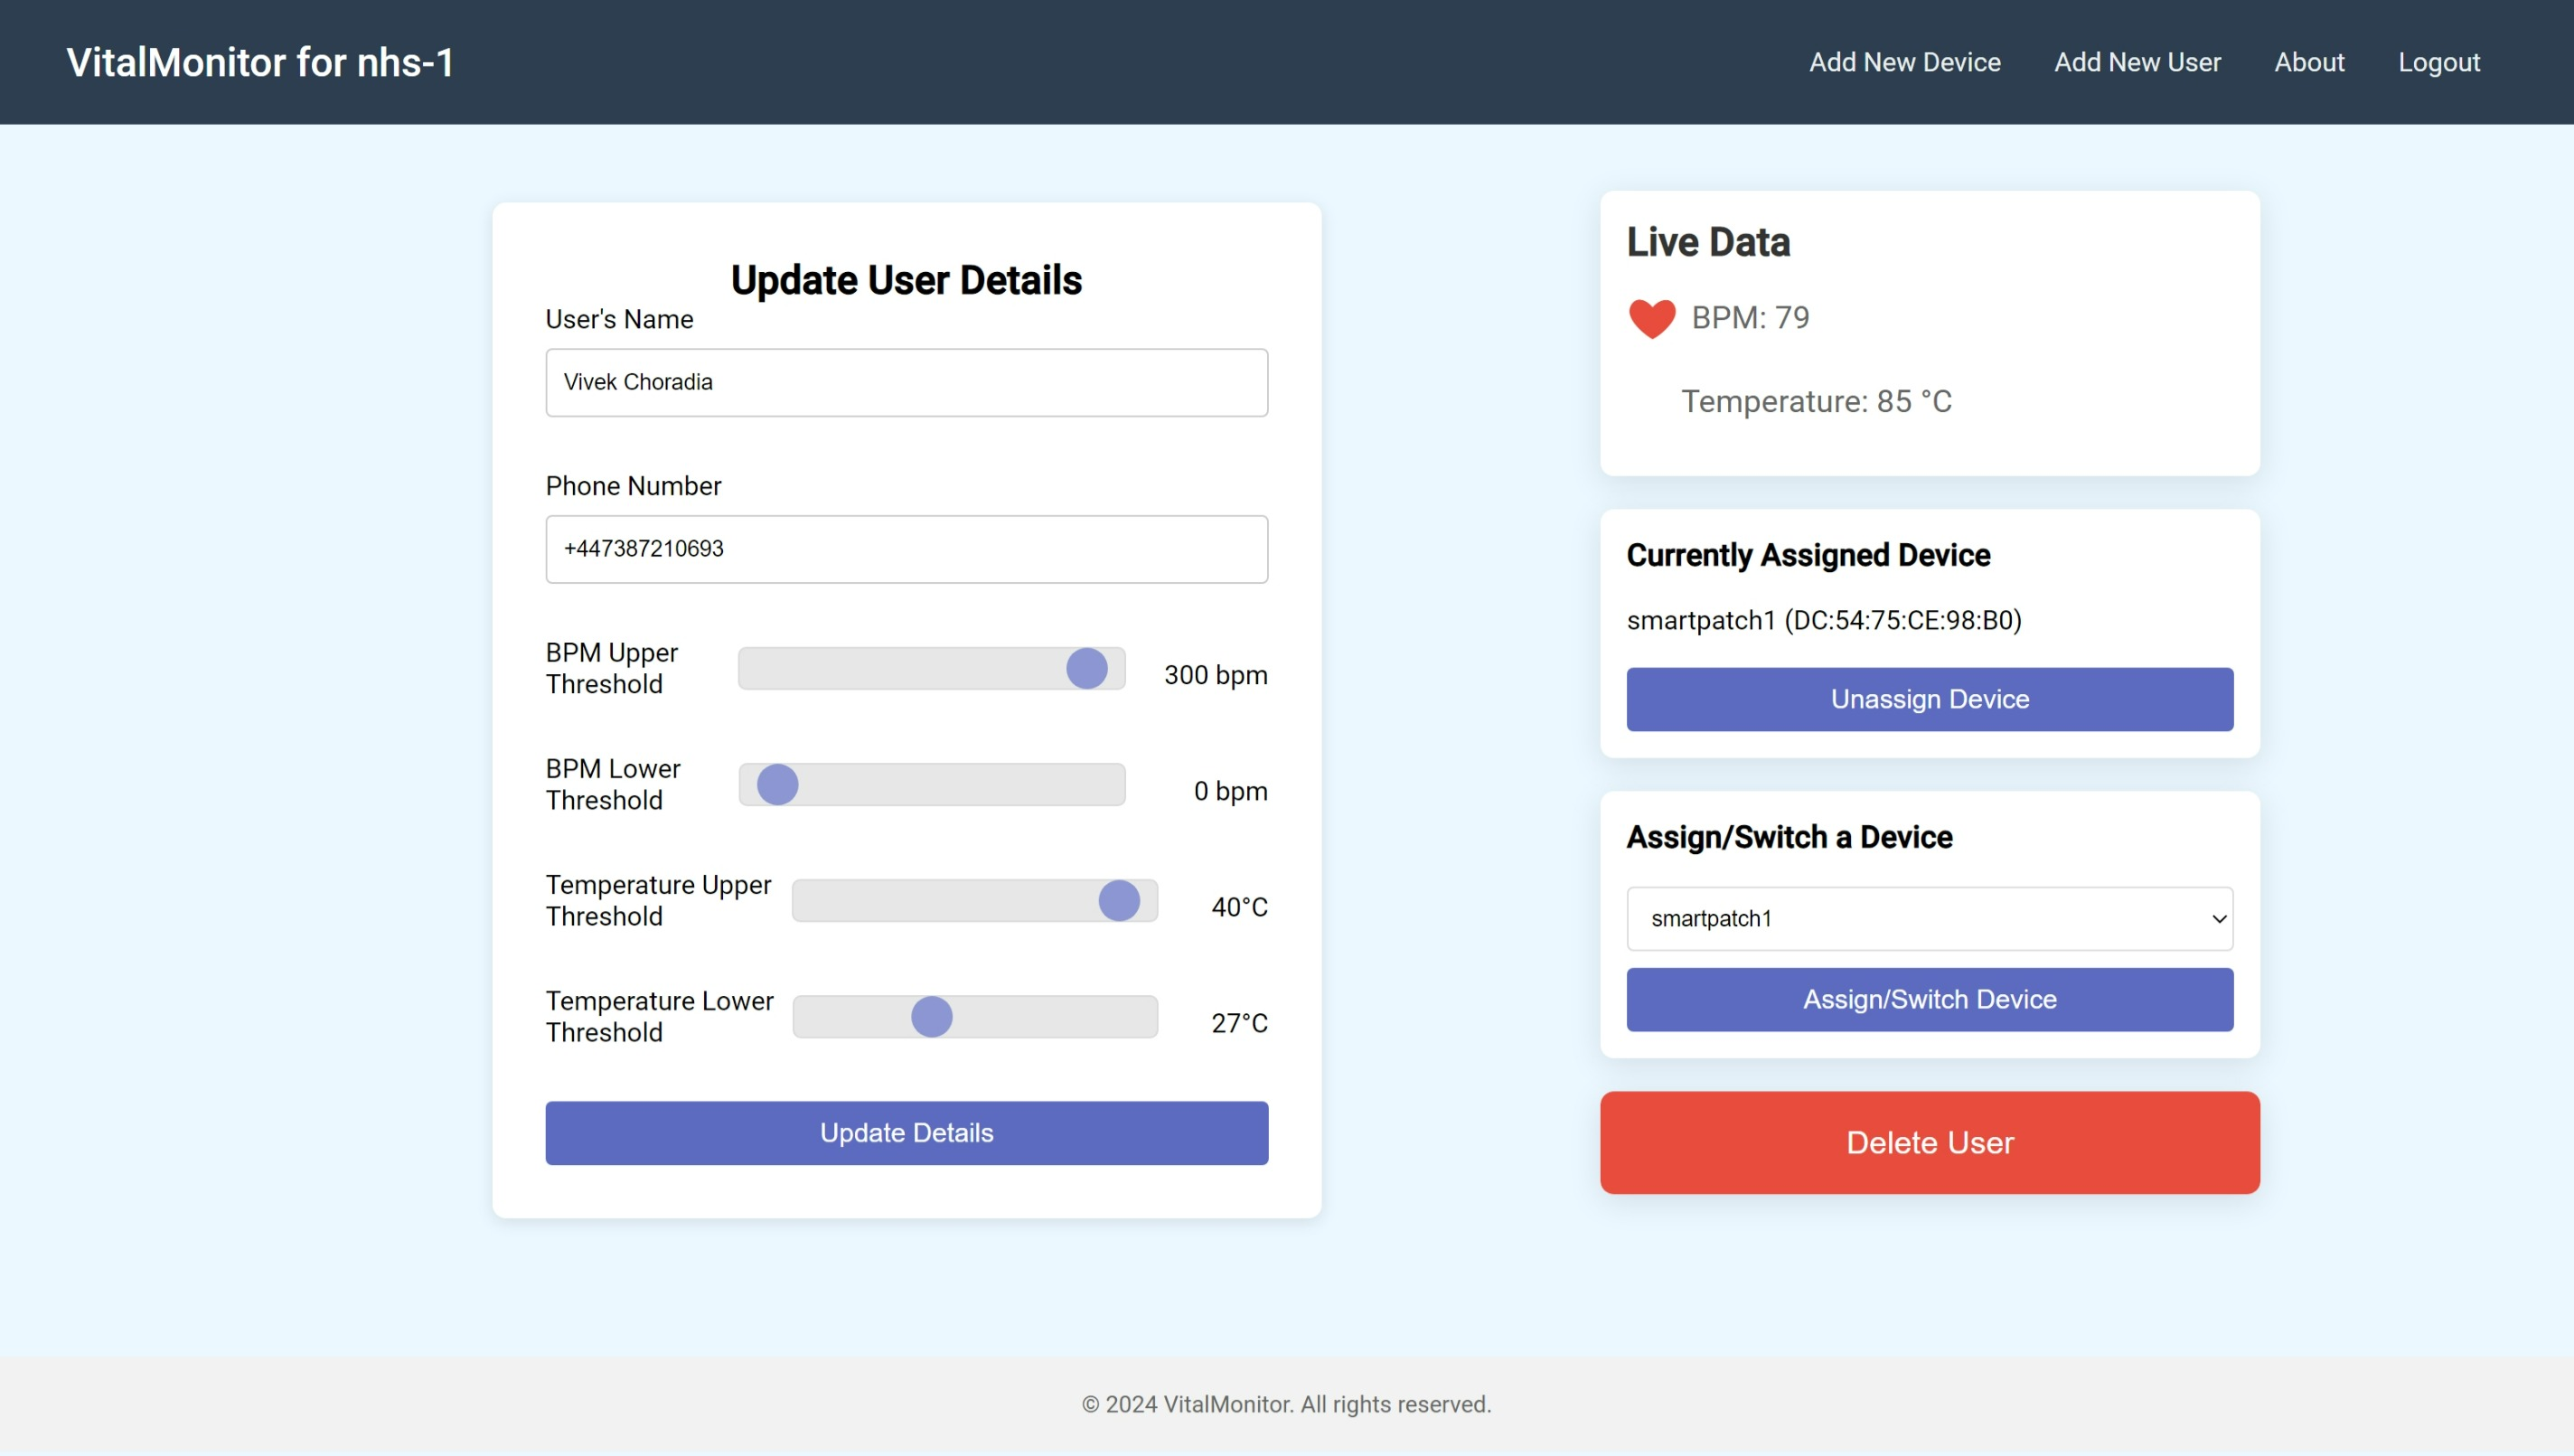
\includegraphics[width=1\linewidth]{images/dashboard-1.jpeg}
    \caption{User Page}
    \label{fig:user-page}
\end{figure}

\begin{figure}[h!]
    \centering
    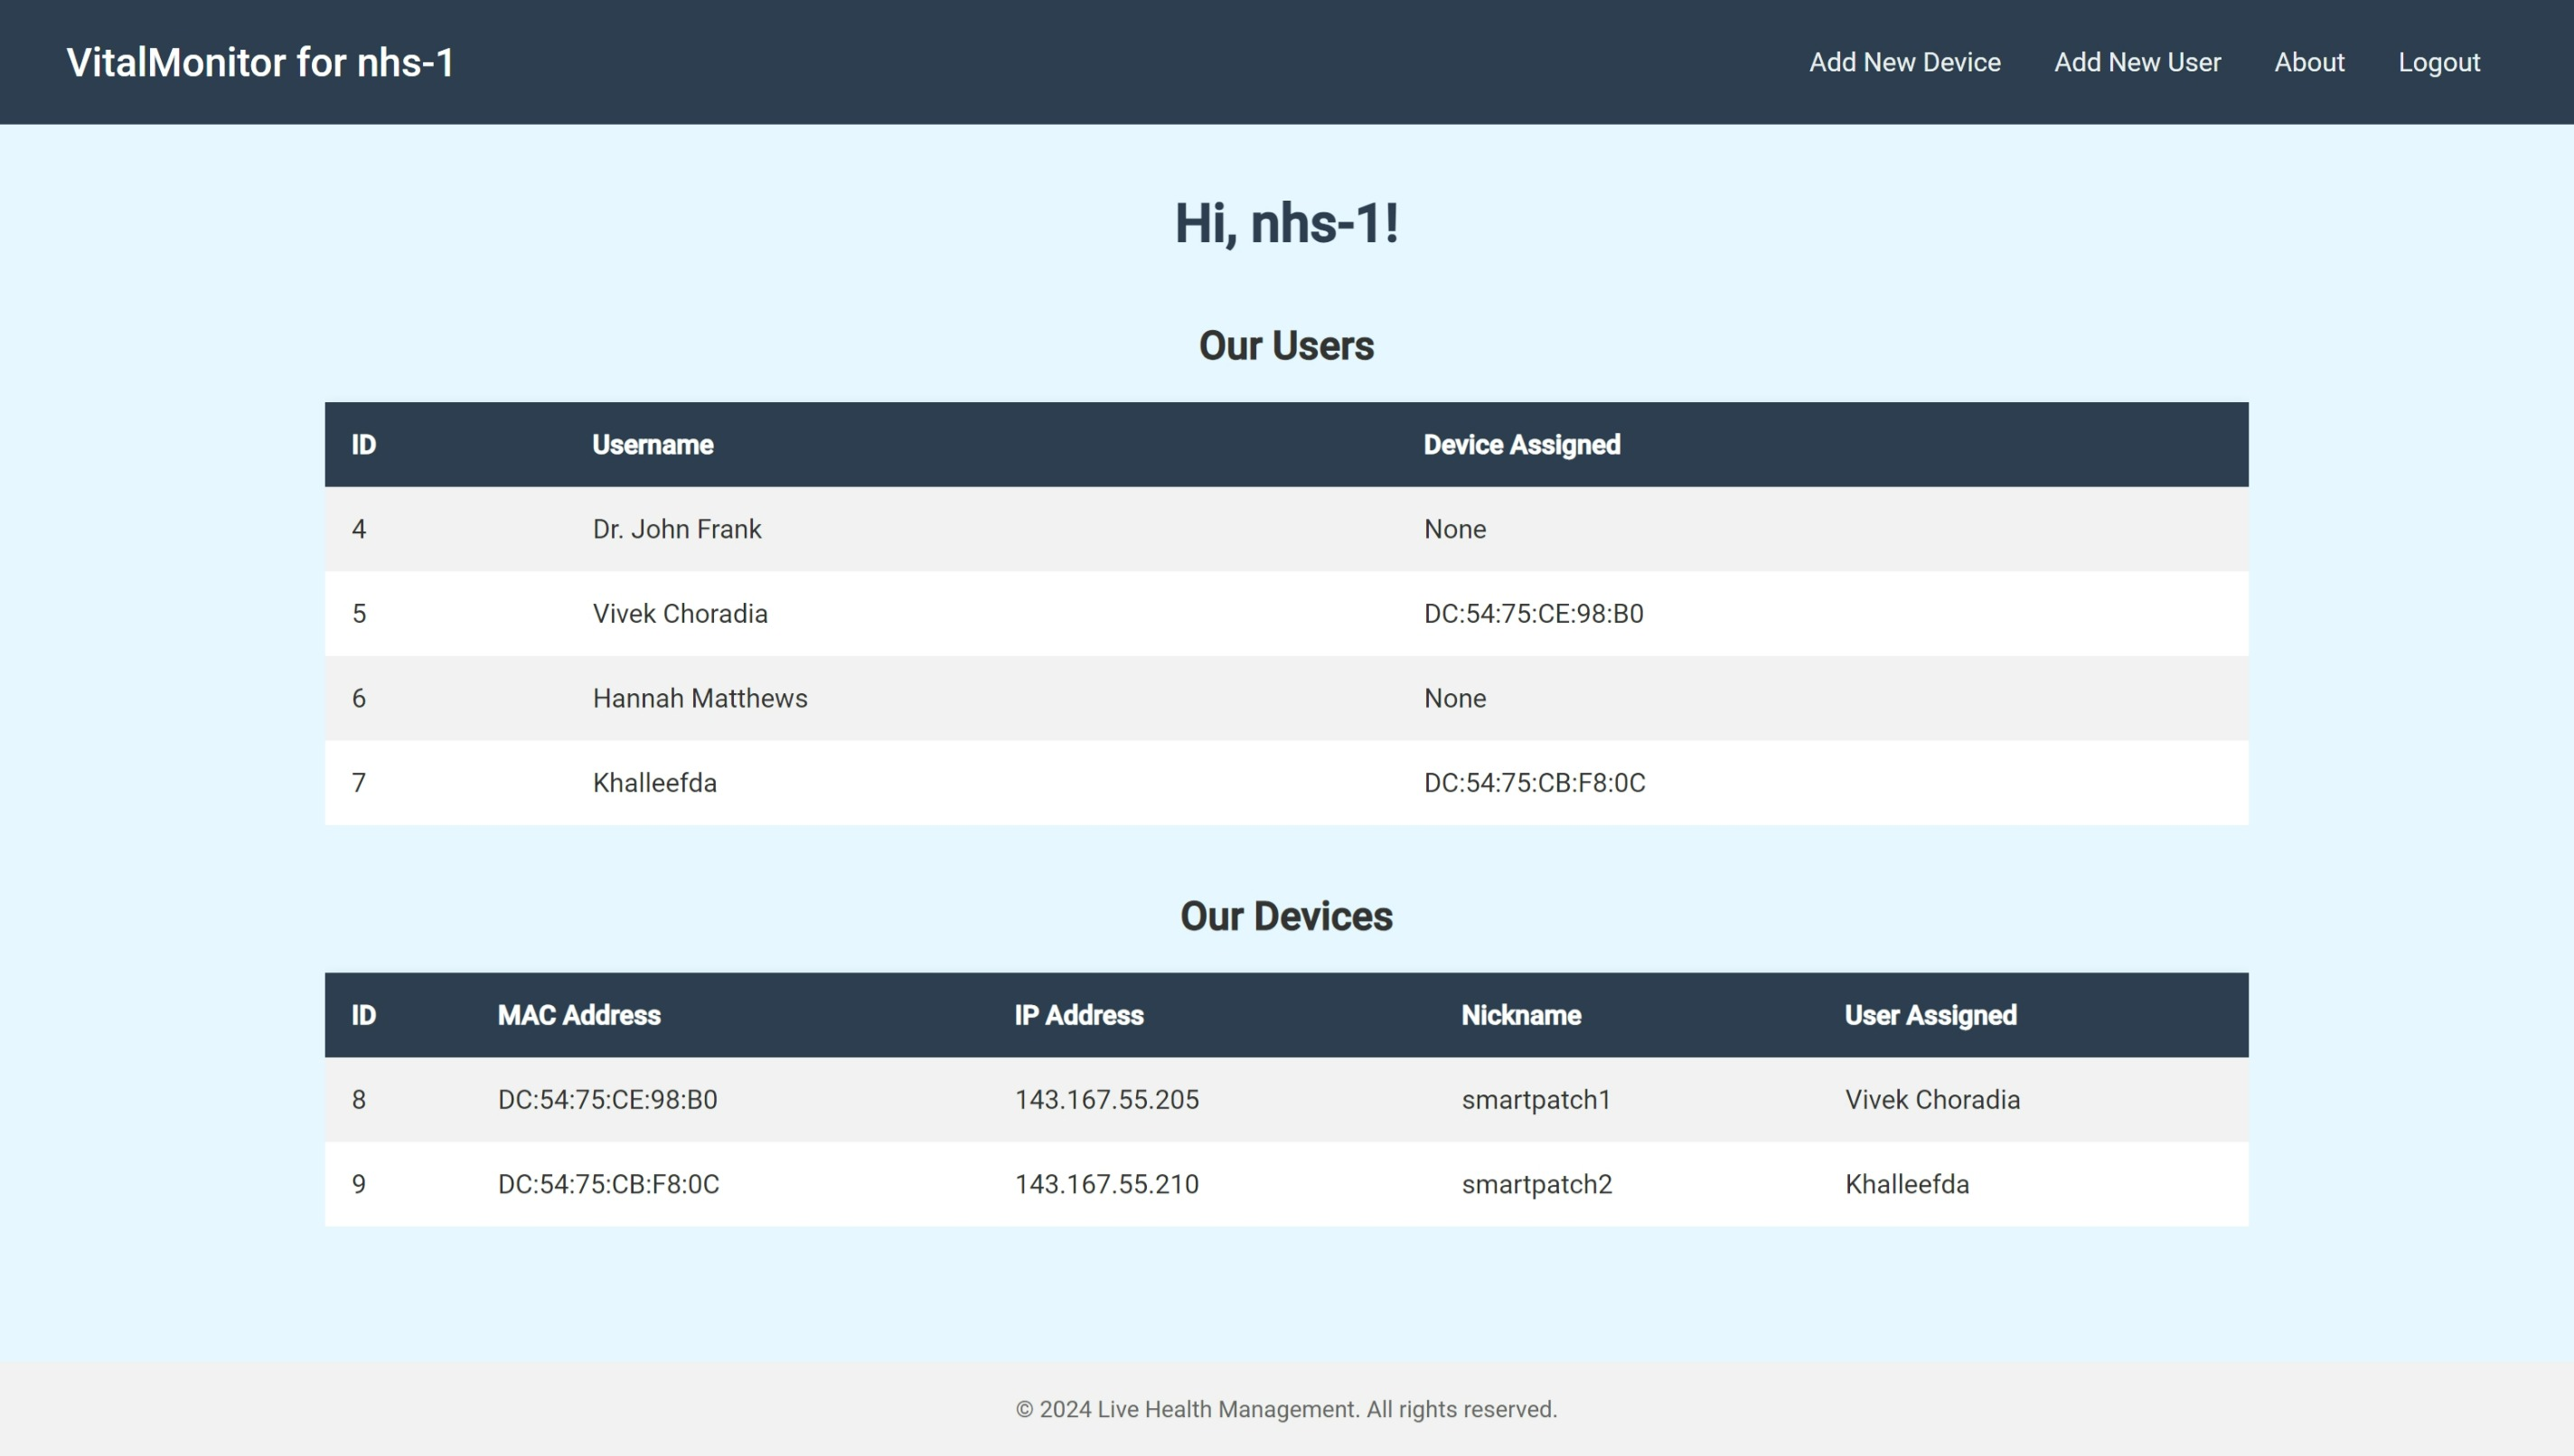
\includegraphics[width=1\linewidth]{images/dashboard-2.jpeg}
    \caption{About Page}
    \label{fig:about-page}
\end{figure}

\clearpage
\section{Testing}
The Testing section details the comprehensive strategies and methodologies used to validate the functionality and reliability of VitalMonitor. This encompasses a range of testing techniques from automated unit and integration tests to manual testing, ensuring the system meets all specified requirements.

\subsection {Acceptance Testing}
Acceptance Testing is important in verifying the system against defined user stories and ensuring that the VitalMonitor functions as intended for end-users. This form of testing is essential for confirming that the system not only functions technically but also fulfills the practical needs of its users. This ensures that the product is ready for deployment and actual use. Each user story is rigorously tested with clear criteria that determine whether the feature is implemented satisfactorily. These tests can be found in the Table \ref{tab:longtable} below.


\begin{longtable}{|c|p{4cm}|p{5cm}|c|}
\caption{User Stories for VitalMonitor Dashboard Implementation} \label{tab:longtable} \\
\hline
\textbf{User Role} & \textbf{Story} & \textbf{Acceptance Criteria} & \textbf{Status} \\ 
\hline
\endfirsthead

\multicolumn{4}{c}%
{{\bfseries Table \thetable\ Continued from previous page}} \\
\hline
\textbf{User Role} & \textbf{Story} & \textbf{Acceptance Criteria} & \textbf{Status} \\
\hline
\endhead

\hline
\multicolumn{4}{|r|}{{Continued on next page}} \\ \hline
\endfoot

\hline
\endlastfoot

Admin & I want to register my organization. & 1. Admin fills and submits a form with organization details. \newline 2. System confirms registration.  & Implemented \\ 
\hline
Admin & I want to log in to the dashboard. & 1. Admin enters credentials. \newline 2. System authenticates and grants access. \newline 3. Error messages are displayed for failures. & Implemented \\
\hline
Admin & I want to add new users. & 1. Admin fills out user form including essential details. \newline 2. Optionally assigns a device. \newline 3. Privacy policy agreement is required for submission. & Implemented \\
\hline
Admin & I want to add new devices. & 1. Admin enters device details. \newline 2. System validates and registers the device. \newline 3. Admin receives confirmation. & Implemented \\
\hline
Admin & I want to manage user-device assignments. & 1. Admin can assign, unassign, or switch devices through user profiles. \newline 2. Updates are immediate and visible. & Implemented \\
\hline
Admin & I want to monitor vital signs in real-time. & 1. Live vital data displayed on user cards. \newline 2. Detailed view available upon clicking a card. \newline 3. Data streams live.  & Implemented \\
\hline
Admin & I want to securely log out. & 1. Admin clicks logout in Navbar. \newline 2. Redirected to login page. \newline 3. Session is cleared.  & Implemented \\
\hline
Admin & I want to view a summary of users and devices. & 1. Admin accesses About Page from Navbar. \newline 2. Page lists all resources. \newline 3. Options for data reporting and exporting available. & Implemented \\ \hline
User & I want to wear the device comfortably on my ear (Future Implementation). & 1. The device is lightweight and designed to fit securely on the ear. \newline 2. Users report comfort and lack of interference with daily activities. & Not Started \\
\hline
User & I want to easily activate the Smart Patch by pressing a button. & 1. The device has a single button for activation. \newline 2. Pressing the button turns on the device and starts data transmission, indicated by a red light. & Implemented \\
\hline
User & I want to press the button again to stop sending data. & 1. Pressing the button a second time turns off the device and stops data transmission, indicated by the red light turning off. \newline 2. Data stops being published immediately. & Implemented \\
\hline
User & I want the device to continuously measure my heart rate and body temperature while activated. & 1. The device measures heart rate and body temperature in real-time. \newline 2. Data is sent to the system at regular intervals without delay while the device is on. & Implemented \\
\hline
\end{longtable}


\subsection{System and Integration Testing}

System and Integration Testing play a crucial role in ensuring the reliability and functionality of VitalMonitor's API endpoints. These tests aim to validate the behavior of the system as a whole and the interactions between its various components. VitalMonitor employs a testing approach, primarily using curl commands to interact with API endpoints. This approach allows for thorough validation of each endpoint's functionality and behavior in different scenarios.  \\

\noindent Various testing scenarios are covered to ensure the robustness of VitalMonitor's API endpoints:
\begin{enumerate}
    \item \textbf{Endpoint Functionality}: Each API endpoint is tested to verify its functionality, including creating, updating, retrieving, and deleting resources such as organizations, users, and devices.
    \item \textbf{Data Validation}: Input data is tested for validity and completeness, ensuring that endpoints handle both valid and invalid data gracefully. This includes testing edge cases and boundary conditions.
    \item \textbf{Error Handling}: Error scenarios are tested to validate the system's behavior when encountering errors, such as missing parameters, unauthorized access, or internal server errors. The responses are examined to ensure they provide meaningful error messages and appropriate status codes.
    \item \textbf{Integration Testing}: Endpoints that interact with external systems, such as devices or external APIs, are thoroughly tested to ensure seamless integration and proper data exchange.
\end{enumerate}

Curl commands are utilized to perform these testings of VitalMonitor's API endpoints. These commands are executed from the command line interface and simulate HTTP requests to interact with the system. One example of such command and the response received is shown in Figure \ref{fig:curl-command}:

\begin{figure}[h!]
    \centering
    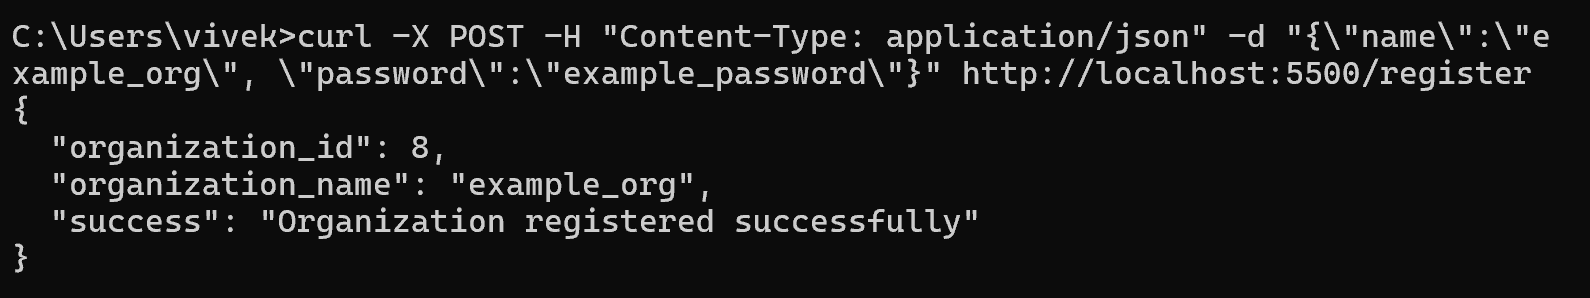
\includegraphics[width=1\linewidth]{images/curl-command.png}
    \caption{CURL Command to test whether adding organization }
    \label{fig:curl-command}
\end{figure}


\subsection{Unit Testing}
Unit testing for both the middleware and the web dashboard was rigorously conducted to ensure robustness and functionality across all components. These tests were implemented using the \textit{pytest} framework and the flask-testing library, supplemented by additional tools such as \textit{contextlib}, \textit{unittest.patch}, \textit{unittest.mock}, \textit{sqlalchemy.exc}, and \textit{requests.exceptions}. This robust toolkit facilitated a comprehensive testing approach, encompassing both functional correctness and error handling capabilities. \\

\noindent To avoid impacting the development database, a dedicated local SQLite database was provisioned for the duration of the testing phase. This temporary database was programmatically created prior to each test suite and subsequently destroyed upon completion, ensuring a clean slate for each test run and preventing data persistence that could skew test outcomes.\\

\noindent Furthermore, in order to fully simulate API interactions without actual external API calls, mock responses and requests were meticulously crafted. This allowed for controlled testing of API functionalities and error handling without the need for live network conditions, thereby increasing the reliability of the test outcomes. However, certain interactions, such as data exchanges with other subsystems, could not be effectively simulated within this framework. These scenarios were addressed through targeted manual testing to ensure comprehensive coverage.\\

\noindent Coverage analysis was conducted using the \textit{coverage.py} tool, providing insights into the extent of code executed by the tests and highlighting any areas lacking in test coverage. This analysis was crucial in identifying untested paths and informed subsequent test development to ensure a high degree of code coverage.\\

The results of these efforts are as follows: 
\begin{itemize}
    \item The middleware was subjected to 37 unit tests, with the coverage outcomes detailed in Figure \ref{fig:middleware-coverage}.
    \begin{figure}[h!]
    \centering
    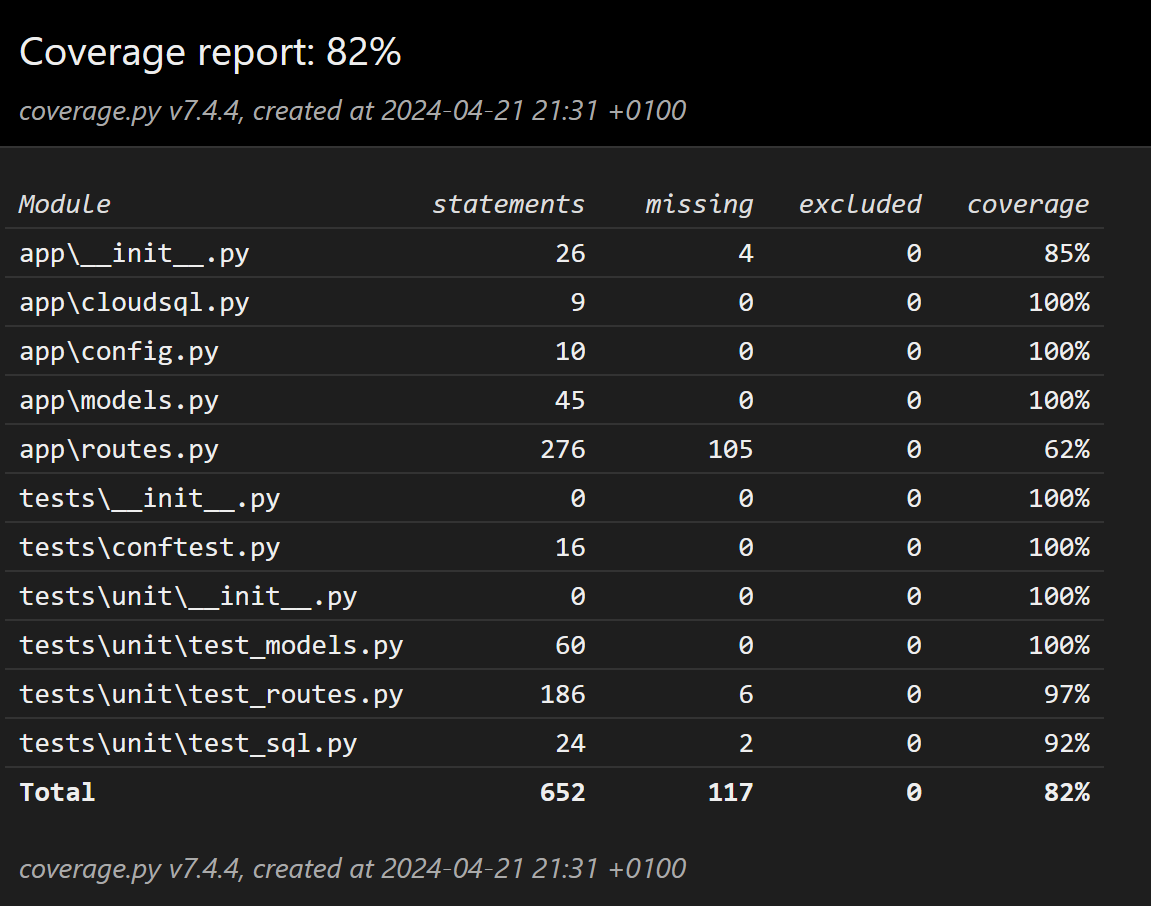
\includegraphics[width=0.7\linewidth]{images/middleware-coverage.png}
    \caption{Middleware Coverage}
    \label{fig:middleware-coverage}
\end{figure}
    \item The web dashboard underwent a series of 27 unit tests, with its respective coverage report depicted in Figure \ref{fig:web-dashboard-coverage}.
    \begin{figure}[h!]
    \centering
    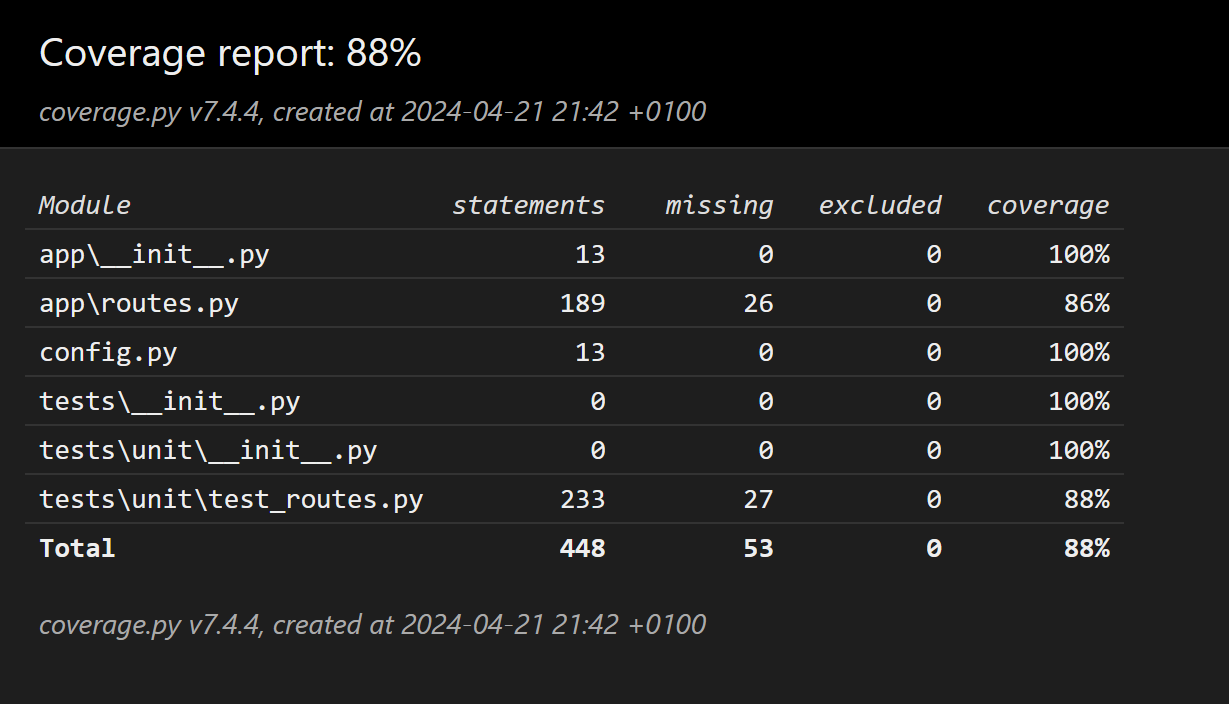
\includegraphics[width=0.7\linewidth]{images/webdashboard-coverage.png}
    \caption{Web Dashboard Coverage}
    \label{fig:web-dashboard-coverage}
\end{figure} 
\end{itemize}



\newpage
\subsection{Manual Testing}

Manual testing was rigorously conducted on both the Web Dashboard and the Smart Patch to ensure comprehensive validation of system functionalities not covered by automated tests. This process is crucial for verifying the integrated operation of all subsystems, offering insights into real-world usability and interaction sequences that automated tests might overlook. \\

\noindent For a structured approach, each test case was assigned a unique Test Case ID, with meticulously detailed test procedures and clearly defined expected results. The outcomes of these tests were diligently recorded, specifying whether each test case passed or failed, thus providing a transparent and accountable testing framework. \\

\noindent The example below illustrates the methodical nature of our manual testing approach:

\begin{longtable}{|c|p{5cm}|p{4cm}|c|}
\caption{Manual Test Cases for Smart Patch Device} \label{tab:manual_tests_device} \\
\hline
\textbf{Test Case ID} & \textbf{Test Details} & \textbf{Expected Results} & \textbf{Pass/Fail} \\
\hline
\endfirsthead

\multicolumn{4}{c}%
{{\bfseries Table \thetable\ Continued from previous page}} \\
\hline
\textbf{Test Case ID} & \textbf{Test Details} & \textbf{Expected Results} & \textbf{Pass/Fail} \\
\hline
\endhead

\hline
\multicolumn{4}{|r|}{{Continued on next page}} \\ \hline
\endfoot

\hline
\endlastfoot

TC-SP01 & Verify activation of the Smart Patch by pressing the button. \newline
- Ensure the device is off. \newline
- Press the activation button. & Device turns on (red light indicator) and starts transmitting data. & Pass \\
\hline
\end{longtable}

A comprehensive list of all manual test cases, along with their respective details and outcomes, is provided in the \textbf{Appendix \ref{app:manual-testing}}. This meticulous documentation facilitates an in-depth understanding of the product’s performance in real-world scenarios and ensures all subsystems function harmoniously together.

\chapter{Results and Discussions}

This chapter presents a comprehensive analysis of the results obtained from the development and implementation of the VitalMonitor. The primary objective was to address existing gaps in healthcare monitoring of HCPs by using IoT and IoTaaS platform to facilitate remote and non-intrusive healthcare solution for HCPs. The findings are evaluated against the project's original aims outlined in Chapter Three, Requirements and Analysis. The final product's demonstration video can be seen \textbf{\href{https://drive.google.com/drive/folders/1X789dsolYtEVA_wNI7RSsXHxpvI9--Kl?usp=sharing}{here}}. This is only accessible by University of Sheffield email address. 

\section{Revisited Requirements}
This project successfully met the majority of its objectives. A prototype of Smart Patch was created. However, the creation of a fully realized product was impeded by several constraints. The prototype is able to get heart rate and body temperature and transmit it in real-time to the dashboard. Additionally, it features functionality to send alerts to emergency contacts via the Twilio API. While the prototype demonstrates substantial capabilities, the transition to a full-scale product would necessitate expertise in electrical engineering and proficiency in CAD for 3D printing. \\

\noindent Aside from the Smart Patch, the IT infrastructure and web dashboard of VitalMonitor has been fully implemented and is operational. The web dashboard is designed specifically for organizational administrators, offers comprehensive functionalities including the ability to add and assign devices to users, among other tasks. These features fulfill all stated project requirements. \\

\noindent During the project's lifecycle, several requirements were revisited and refined to better align with the evolving technological landscape and user feedback. This adaptive approach was pivotal in addressing unforeseen challenges and leveraging new opportunities as they arose. A notable adjustment was the substitution of the LM35 temperature sensor with the DS18B20 sensor. This change was motivated by the digital output capabilities of the DS18B20, which facilitate easier data integration and enhance the accuracy of measurements. \\
 
\begin{figure}
    \centering
    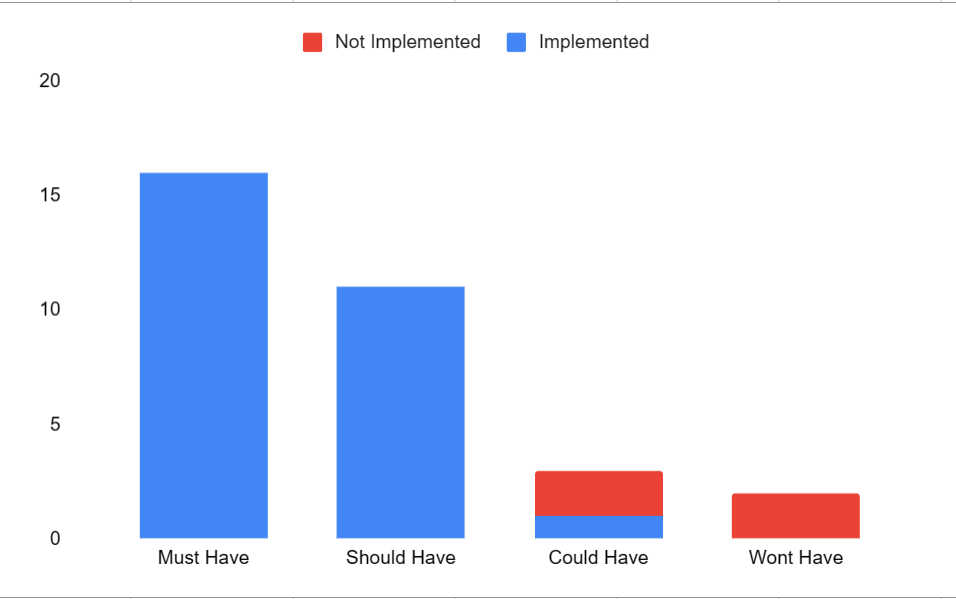
\includegraphics[width=1\linewidth]{images/revisitedr.png}
    \caption{Overview of Requirements post development}
    \label{fig:revisited-requirements}
\end{figure}

\section{Project Cost}
The funding required to design, implement, and test the entire project was substantial and supported by the Department of Computer Science. Monitoring the expenses associated with the prototype provides insights into potential costs of a fully developed product. Minimizing these costs is critical for promoting adoption by healthcare organizations, potentially alleviating their financial constraints. \\

\noindent A detailed overview of the project's expenditures is provided below to ensure transparency in the allocation and utilization of resources:

\begin{table}[h!]
    \centering
    \begin{tabularx}{\textwidth}{|X|c|}
    \hline 
         \textbf{Item}& \textbf{Cost(£)}  \\ \hline
        Pimoroni Pulse Sensor x 2    &  42 \\ 
        LM-35 Sensor & 6.24 \\ 
        ESP32-S3-MINI-1 & 21.00 \\
        DS18B20 & 3.50 \\
        Miscellaneous Components & 4.59 \\ \hline
        Total Hardware Cost & \textbf{56.33} \\ \hline
        
    \end{tabularx}
    \caption{Project Cost}
    \label{tab:project-cost}
\end{table}

Additional Costs:

\begin{itemize}
    \item Utilization of \$55 from Google Cloud's \$300 free credits for development purposes. Cost per day to run the database on Google Cloud with current configurations are \$0.4/day.
    \item Employment of the AdafruitIO free tier, which includes access to 2 dashboards and 10 feeds — sufficient for this project phase.
    \item Allocation of \$12 from a Twilio trial credit to purchase a UK phone number, with each text message incurring a cost of \$0.0420.
\end{itemize}


\section{VitalMonitor's IT Infrastructure}

VitalMonitor has been designed and implemented with scalability and versatility as foundational principles. The IoTaaS platform enables registration for multiple organizations, each of which can support numerous users. VitalMonitor is engineered to easily incorporate additional sensors and functionalities, enhancing its capacity to monitor parameters indicative of fatigue or stress levels. \\ \\
A significant development was the introduction of middleware, which expanded the adaptability of VitalMonitor. Originally conceived to operate within a single hospital's local network, the middleware now facilitates the connection of Smart Patches across diverse network environments. In future iterations, incorporating a System on Chip (SoC) with an integrated SIM card could enable autonomous network connectivity, allowing data to be sent directly to middleware hosted on cloud services such as Google Cloud. This feature would allow organizational administrators to access the dashboard from any location, greatly enhancing the system's utility. \\ \\
Such flexibility extends the potential applications of the product to include healthcare providers in ambulances, natural disaster response teams, and medical camps in remote areas. This adaptability underscores the advanced capability of VitalMonitor to meet a wide range of healthcare monitoring needs, making it a highly versatile and indispensable tool in diverse medical contexts.

% VitalMonitor is designed and implemented to be scalable and versatile.  Many organizations can register themselves to use the IoTaaS platform. And each organization can have multiple users registered. These both depends on the database access VitalMonitor has during the production stage. VitalMonitor can easily be scaled to add more sensors and functionalities like xyz to enhance the parameters used to indicate fatigue or stress level. During the development, adding a middleware - gave path to making VitalMonitor more versatile and adaptable. Initially VitalMonitor was thought of just for a hospital which is on the same local network and all the Smart Patch will be connected directly to the dashboard. But during the development, middleware made it possible to have Smart Patches on different networks as well. And more over when in the next iteration if we choose an SoC which has sim card on it - it can get connected to its own network. And these can directly send data to middleware hosted on google cloud for eg. and the organization's admin can access the dashboard from anywhere it is needed. This extends the number of use cases this product could have - it can be used for HCPs in ambulances, natural disaster relief teams, HCPs in medical camps in a remote place, etc. This feature makes VitalMonitor so much more versatile and adapatable.  



\section{Prototype of Smart Patch}
Smart Patch was implemented keeping in mind its primary objective of being the device that doesn't hinder HCPs in their everyday work. Smart Patch's prototype was made in this iteration of the project. The prototype was specifically designed and developed using sensors which serve this theme. It is able to detect vitals of HCP in the least intrusive and most remote way. It runs its own mini asynchronous web server to transmit the data to middleware server. Additionally, a manual switch is incorporated, empowering the wearer to control when data is recorded. Only when the wearer (here HCP) presses the switch and red LED turns on - only then the data is measured. \\ \\
The ergonomic design of the device, strategically positioned behind the ear, and the selection of sensors were dictated by the need for comfort and the physiological requisites for precise data collection. This stage of the project did not focus on finalizing the product design; thus, further development involving 3D printing and product optimization is required. Time constraints in this phase prevented the advancement to a finalized product.


\begin{figure}[h!]
    \centering
    \begin{subfigure}[b]{0.45\linewidth}
        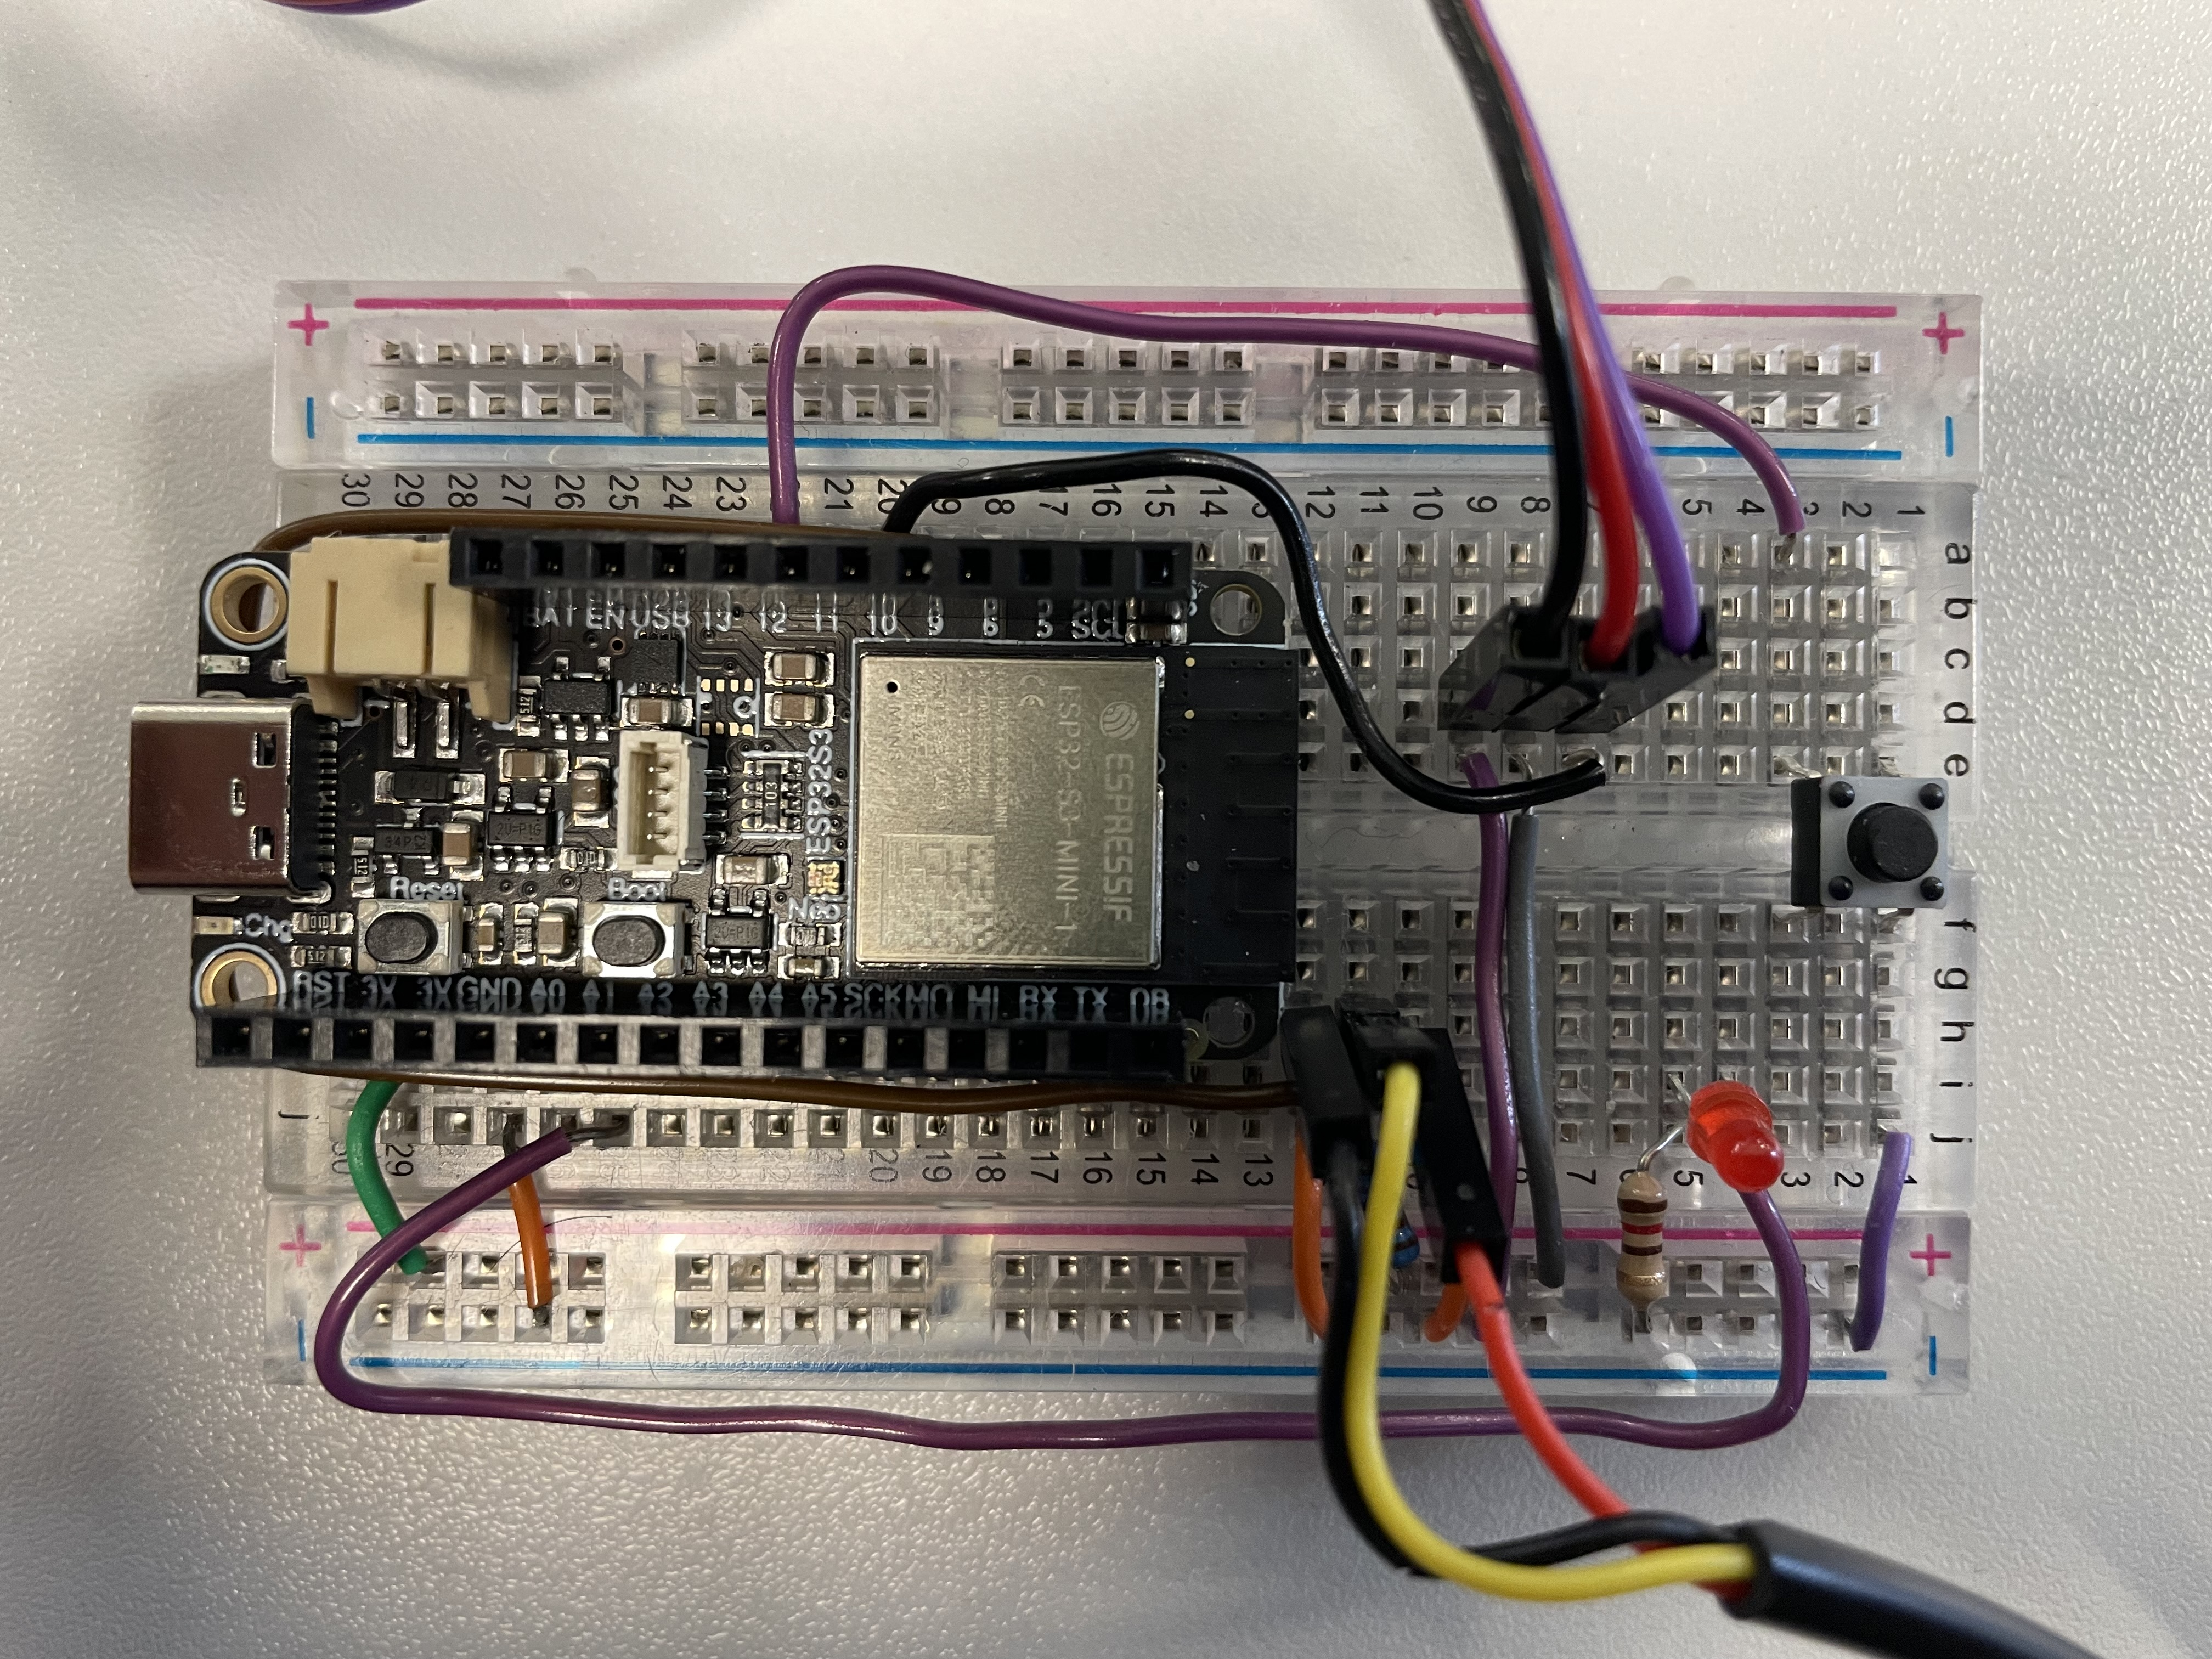
\includegraphics[width=\linewidth]{images/v6-hardware.jpg}
        \caption{Prototype}
        \label{fig:fig-proto}
    \end{subfigure}
    \hfill
    \begin{subfigure}[b]{0.45\linewidth}
        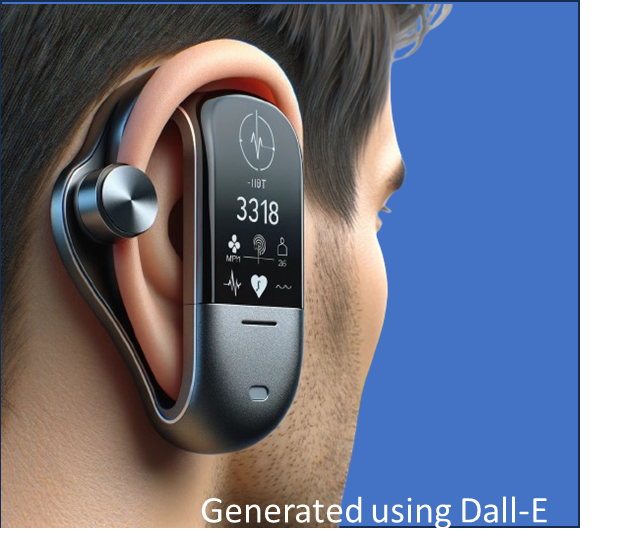
\includegraphics[width=\linewidth]{images/dall-e.png}
        \caption{Design Idea of Physical Product}
        \label{fig:fig-design}
    \end{subfigure}
    \caption{Smart Patch}
    \label{fig:fig-smartpatch}
\end{figure}

\section{Limitations and Issues Encountered}

\subsection{Trade off between Sensor Accuracy and Non-Intrusiveness}
In developing wearable devices for continuous monitoring, a significant challenge is balancing sensor accuracy with the need for non-intrusiveness, particularly for healthcare professionals (HCPs) who wear these devices during long shifts. High accuracy in sensors is crucial, as it ensures that the data collected is reliable enough to inform meaningful interventions to support HCP well-being. However, achieving this often requires more invasive technologies that may interfere with the daily activities and comfort of these professionals.\\ \\
VitalMonitor focuses on optimizing this balance by selecting sensors that minimize intrusiveness while still providing sufficiently accurate data for passive monitoring. This approach is critical in settings where both the well-being of HCPs and operational efficiency are prioritized. Given the limited availability of sensors that strike a perfect balance between non-intrusiveness and high accuracy, the selection was guided by the goal of maintaining user comfort and system reliability. This ensures that healthcare administrators can effectively monitor and respond to the health indicators of their staff without causing discomfort or disruption to their work.

\subsection{Settings Get Lost When Power Goes Off}
The Smart Patch operates by assigning itself to a user through the dashboard. Once the assignment is complete, user data is received by the device. Publishing data only starts when the switch is pressed on the device. However, once the Smart Patch loses power, all assigned data is lost.\\

\noindent To mitigate this issue, the flash memory available in the ESP32 is utilized. EEPROM (Electrically Erasable Programmable Read-Only Memory) is used to save essential data, so the admin does not need to reassign the Smart Patch to a user after power loss. EEPROM is a non-volatile memory technology that retains important data unless the user is deleted or the device is unassigned or switched.\\

\noindent When the device powers on, it first checks for saved information or settings. If data already exists, it will resume publishing data as previously configured. Here is a code snippet illustrating how EEPROM is used in the setup process:

\begin{lstlisting}[language=C++, caption={Using EEPROM in Setup()}, label={EEPROM_in_setup}]
  if (!EEPROM.begin(512)) { 
    Serial.println("Failed to initialize EEPROM");
    return;
  }

  DeviceSettings settings = loadSettings(); 
  global_name = settings.name;
  global_to = settings.phoneNumber;
  global_bpm_lower_threshold = settings.bpmLowerThreshold;
  global_bpm_upper_threshold = settings.bpmUpperThreshold;
  global_temp_lower_threshold = settings.tempLowerThreshold;
  global_temp_upper_threshold = settings.tempUpperThreshold;
  global_isPublishing = settings.isPublishing;

\end{lstlisting}

This approach ensures that critical settings stay in the Smart Patch unless explicitly changed.

\subsection{Converting Raw Data to Useful Data}

The DS18B20 Temperature Sensor and Pimoroni Pulse Sensor are integral to VitalMonitor's functionality, changing analog electrical signals into digital data for health monitoring. However, this reading process often introduces significant noise, resulting in irregular and unreliable data outputs.  Such anomalies, if unaddressed, could potentially trigger unwarranted alarms or actions based on incorrect information. This necessitates robust data processing strategies to ensure accuracy and usability. \\ \\
A common challenge in sensor data analysis is managing these irregularities, particularly when they lead to significant deviations from expected patterns. For example, an abrupt spike in temperature readings from 32 degrees Celsius to an erroneous 45 degrees could inadvertently exceed the system’s threshold of 35 degrees, resulting in false alarms. To ensure data integrity and reliability, it is imperative to employ robust data smoothing techniques. \\ \\
The Moving Average filter is one such technique applied within the VitalMonitor framework. By averaging data points over a defined time window, this method effectively dampens the impact of transient spikes or noise, leading to a more stable and accurate data output. This technique not only enhances the overall quality of the health monitoring data but also supports critical decision-making processes by reducing the likelihood of false alerts. Figure \ref{fig:data-sensors} provides a snapshot of data collected from the sensors in their raw form as well as data after implementing Moving Average function to it. \\

\begin{figure}[h!]
    \centering
    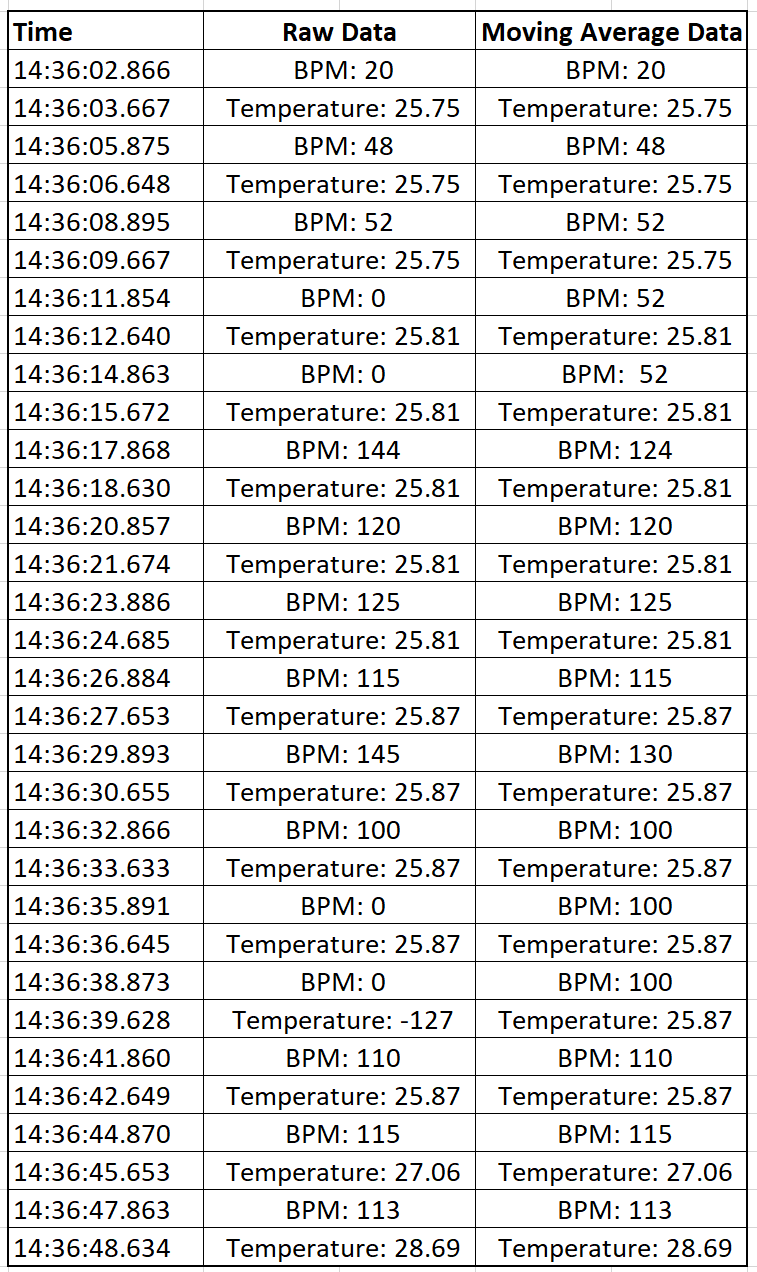
\includegraphics[width=0.6\linewidth]{images/data.png}
    \caption{Data from sensors}
    \label{fig:data-sensors}
\end{figure}

\noindent Extensive testing and evaluation have confirmed that the adapted sensors provide a data precision of \(\pm 15\) BPM for heart rate and \(\pm 0.2-0.5\) degree Celsius for temperature. These measures ensure that VitalMonitor delivers reliable and actionable health data for healthcare professionals, enhancing the monitoring and management of their well-being.

\subsection{Reliability depends on Network Bandwidth}
The effective operation of VitalMonitor’s Smart Patches heavily relies on the strength and capacity of the WiFi network to which they are connected. These devices are designed to upload data in real-time, a process that demands robust network performance to function seamlessly. With a scenario involving up to 100 Smart Patches transmitting data simultaneously, the bandwidth requirements become substantial. This substantial demand can strain the network, leading to potential data transmission delays that may impact the timeliness and reliability of data being displayed on the monitoring dashboard. \\ \\
During extensive testing and evaluation, it was observed that the system's reliability is significantly influenced by the WiFi network's bandwidth. Insufficient bandwidth can result in lagging data updates, which may hinder the system’s ability to provide real-time insights crucial for immediate decision-making and response. This finding underscores the necessity for implementing a network infrastructure capable of supporting high data loads, especially in environments where continuous and simultaneous monitoring is critical. Efforts to enhance network configurations, possibly through dedicated channels or enhanced WiFi protocols, are essential to mitigate these issues and ensure reliable system performance.

\subsection{Google Cloud}
Google Cloud offers \$300 in credits for database and server usage. In this project iteration, these credits were primarily utilized for the MySQL database, specifically the Enterprise Cloud SQL Edition. The chosen configuration, as depicted in Figure \ref{fig:cloud-configurations}, was optimized for cost efficiency, with an initial setup cost of \$6 and a daily operational cost of \$0.4. While suitable for development and testing purposes, this configuration may prove inadequate for production deployment, particularly when supporting a larger user base. \\

\begin{figure}[h!]
    \centering
    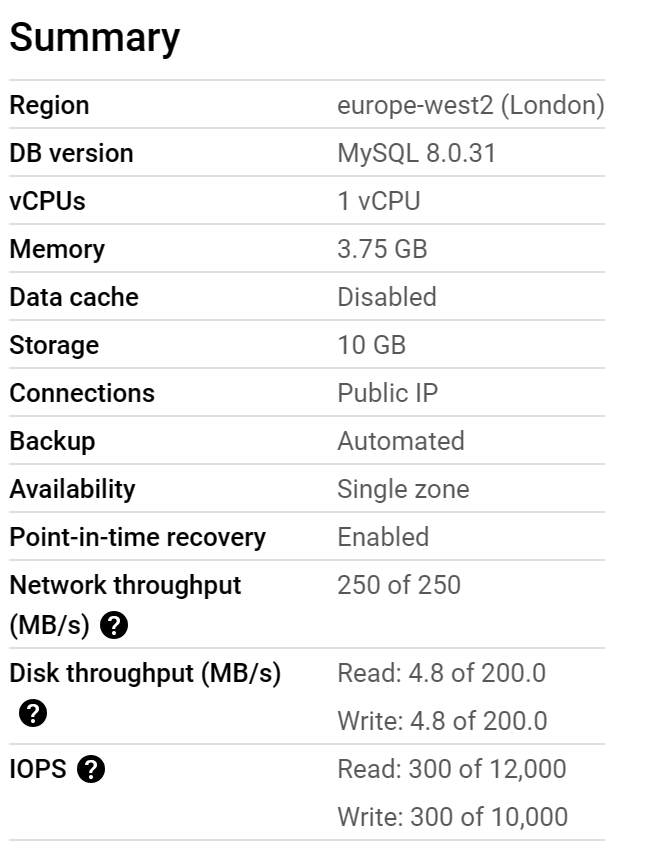
\includegraphics[width=0.5\linewidth]{images/cloud-configurations.png}
    \caption{Google Cloud Configurations}
    \label{fig:cloud-configurations}
\end{figure}

\noindent In a production environment scenario accommodating 100 HCPs and a single dashboard for hospital, upgrading database to the Enterprise Plus Cloud SQL Edition becomes imperative. This entails provisioning a minimum of 8 virtual CPUs, 32 GB of RAM, and increasing storage capacity to over 100 GB. Additionally, as the platform scales to serve multiple hospitals, resource requirements will escalate accordingly.\\

\noindent Furthermore, the middleware microservices will be deployed on Google Cloud in the production phase. These services interact with the database through HTTPS requests, utilizing unix-sockets with appropriate permissions. For instance, when an administrator adds a new device via the dashboard, the workflow involves traversing through the web page, web server, middleware, and database (hosted on Google Cloud) before returning. While deploying middleware on Google Cloud can streamline transactions and improve response times, it necessitates additional costs. Hence, this optimization was deferred in the current iteration to maintain cost-effectiveness.


\section{Further Work}
Despite having achieved the core objectives and beyond, there are more enhancements that this project could have done if not for the time constraint and knowledge-specific constraint. Further Work are divided into 3, things to be done to create a minimum viable product, improving current implementations and finally adding new requirements to make VitalMonitor more efficient.

\subsection{Smart Patch: Final Product}
The culmination of the Smart Patch project will yield a refined, compact device designed to discreetly rest behind the ear. This final iteration will feature optimized sensor placement, with the pulse sensor delicately positioned on the earlobe and the temperature sensor situated inconspicuously behind the ear. Transitioning from the current breadboard prototype to a fully soldered device with a 3D-printed cover will be pivotal, streamlining the product for mass production and enhancing its durability. A sample design was created for future device using Dall-E. This design is shown in Figure \ref{fig:fig-smartpatch}. Refer to Appendix \ref{chatgpt-prompts} for more information on how this image was generated. 

\noindent To achieve this, future efforts will focus on miniaturizing the device through advanced CAD design and employing more efficient microcontroller tailored specifically for the Smart Patch. However, before deployment, rigorous testing, including Electrical Safety Testing and Mechanical/Physical Testing, will be necessary to ensure compliance with industry standards and user safety. Although these tests were not feasible within the project's constraints, they remain critical future steps to validate the device's reliability and regulatory compliance.


\subsection{Improving the Middleware Infrastructure}
In future, the Middleware Infrastructure can be transitioned from a monolithic architecture to a more scalable and robust system comprising four distinct microservices. Currently, the infrastructure operates as a single web server, but the proposed evolution involves isolating functionality into four dedicated microservices: Session Management Service, User and Device Management Service, Data Ingestion Service, and Data Retrieval Service. By segmenting these services across different web servers, the workload is distributed more evenly, reducing the strain on any single server and enhancing system efficiency. \\ \\
This architectural enhancement not only fosters a clearer separation of concerns but also facilitates improved request management and scalability. Implementing a load balancer to orchestrate requests among these microservices ensures efficient data flow, minimizing the risk of data loss and optimizing overall system performance. This strategic restructuring lays the foundation for a more resilient and adaptable Middleware Infrastructure, poised to accommodate future growth and evolving user demands.

\subsection{Algorithm to Measure Stress and Fatigue Levels}
Existing methodologies lack a standardized approach to real-time measurement of stress and fatigue, primarily due to their multifaceted nature, influenced by a multitude of physiological and psychological factors. To address this challenge, further research is essential to develop an algorithm capable of quantifying these parameters quantitatively. This algorithmic approach aims to integrate various vital signs and personal information, providing a more comprehensive understanding of individual well-being beyond subjective descriptors like ``very stressed." Collaboration with medical researchers will be pivotal in discerning relevant parameters and assigning appropriate weights based on empirical evidence. By leveraging insights from medical literature and empirical data, the project will look in to refining decision-making processes and enhance the precision of stress and fatigue assessments. \\ \\
The ultimate goal is to streamline healthcare interventions and reduce reliance on simplistic thresholds, fostering a more nuanced approach to individual well-being monitoring. Although this entails extensive data gathering and analysis, its potential to expedite decision-making processes and improve healthcare outcomes underscores its significance in the realm of healthcare monitoring for HCPs.

\subsection{Interdisciplinary Collaboration for Enhanced Sensors}
Addressing the inherent trade-off between sensor accuracy and non-intrusiveness, it is neccessary to have interdisciplinary collaboration by electrical engineers and bio-medical engineers in this project. By pooling expertise from both fields, development of enhanced sensors will take place. These sensor(s) will be capable of accurately measuring vital signs such as heart rate and body temperature, while remaining non-intrusive to wear. This collaborative effort holds the potential to disrupt the healthcare industry by introducing innovative sensor technologies that prioritize both accuracy and user comfort.\\ \\
The development of non-intrusive sensors not only meets the demands of HCPs but also enhances the overall experience for patients undergoing medical treatments. By minimizing discomfort associated with traditional monitoring methods, non-intrusive sensors offer a more patient-centric approach to healthcare delivery, ultimately alleviating suffering and improving the quality of care. This interdisciplinary collaboration represents a pivotal step towards realizing the full potential of sensor technology in revolutionizing healthcare monitoring and patient outcomes.

\subsection{Prediction Model}
Stress and fatigue often rise gradually, with occasional spikes triggered by unforeseen events or stressors. Recognizing this pattern, future iterations will aim to develop a prediction model trained on actual human data. By forecasting stress levels before they surpass predetermined thresholds, this model provides early warning signals to healthcare organization administrators. Such anticipatory measures afford administrators more time to make necessary arrangements, mitigating the impact of heightened stress levels on healthcare professionals (HCPs) and optimizing patient care.\\\\
The integration of predictive analysis represents a notable advancement, augmenting VitalMonitor with cutting-edge AI and analytics functionalities. This strategic augmentation not only distinguishes the platform from competitors but also empowers healthcare organizations with foresight capabilities.
% \newpage

\chapter{Progress}

This section provides a comprehensive overview of the progress made by the project and the ongoing activities of the project. Below are the listed:

\begin{itemize}
    \item \textbf{Getting familiar with embedded systems:} Engaged in practical exercises from the Unphone: IoT book to build a foundational understanding of embedded systems. 
    \item \textbf{Getting familiar with Platform IO and MicroPython:} Currently getting familiar with the development environment and the programming language for effectively programming the Smart Patch.
    \item \textbf{Training}
    \begin{itemize}
        \item \textbf{iForge Training:} Completed iForge basic training and laser cut training. Will be finishing soldering training and 3D printing training by the end of December. 
        \item \textbf{Ethics Review Training:} Participated in ethics review training, ensuring that project activities aligned with ethical standards and guidelines.
    \end{itemize}
    \item \textbf{Scheduling Interviews:} In the process of scheduling interviews and preparing a list of questions to be asked in the interview. Coordinating with the interviewers to have the interviews sometime in January. 
    \item \textbf{Data Flow Diagram:} Developed a data flow diagram to visualize the movement and processing of information within the project, aiding in identifying key interactions and dependencies. Figure \ref{fig:data-flow-1} represents how data will be transmitted from an HCP to Smart patch and Figure \ref{fig:data-flow-2} represents how data collected by Smart patch will be transmitted to the dashboard in real-time. 
    
\begin{figure}
    \centering
    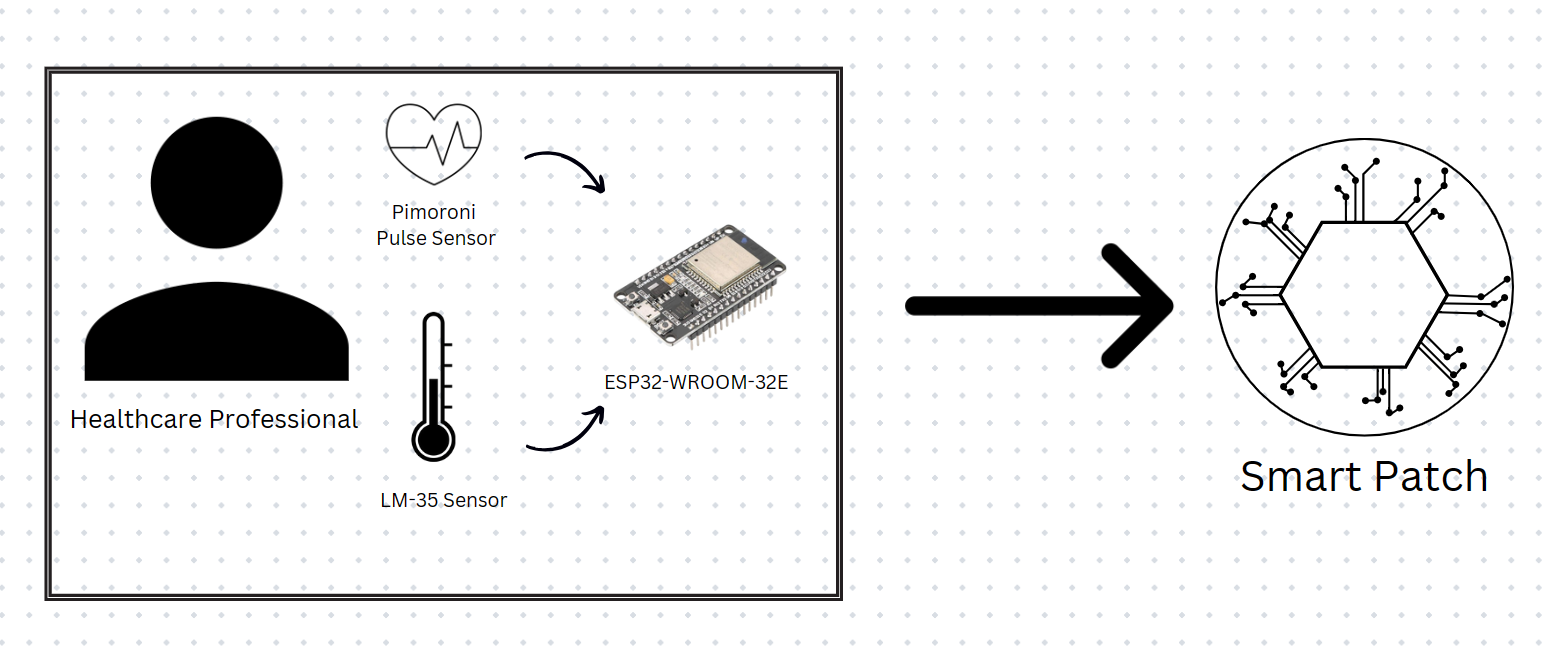
\includegraphics[width=\linewidth]{images/data-flow-1.png}
    \caption{Data Flow Diagram - 1 (From HCP to Smart Patch)}
    \label{fig:data-flow-1}
\end{figure}

\begin{figure}
    \centering
    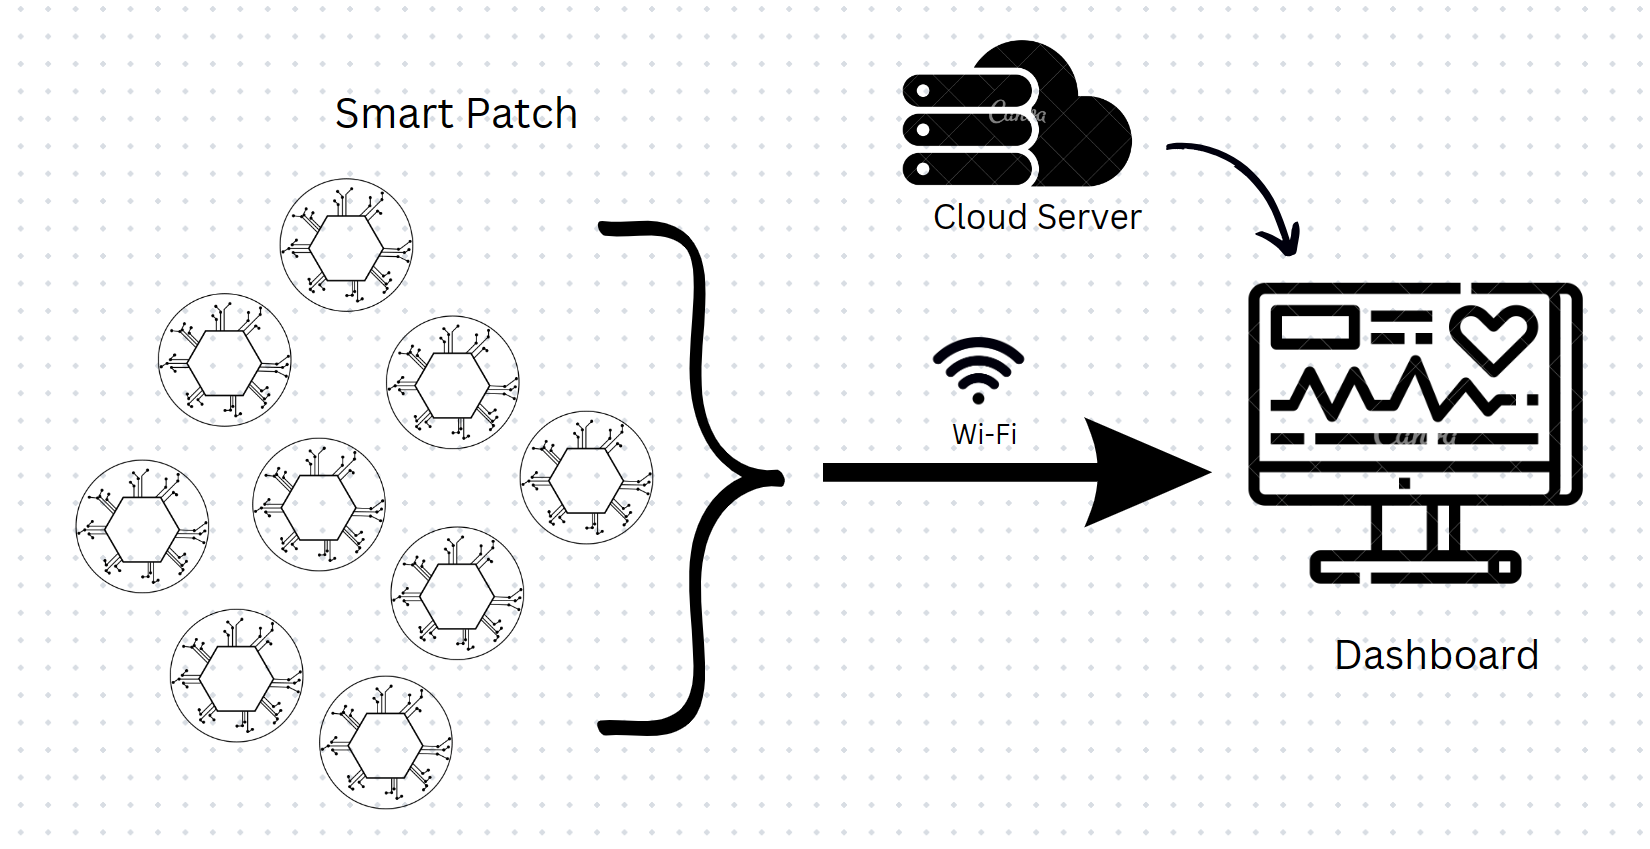
\includegraphics[width=\linewidth]{images/data-flow-2.png}
    \caption{Data Flow Diagram - 2 (From Smart Patch to Dashboard)}
    \label{fig:data-flow-2}
\end{figure}
    
    \item \textbf{Project Plan:} Established a comprehensive project plan using a Gantt Chart, providing a visual timeline of tasks and milestones to guide project execution and monitor progress. This project plan is laid out in Figure \ref{fig:gantt-chart}.

    \begin{figure}
        \centering
        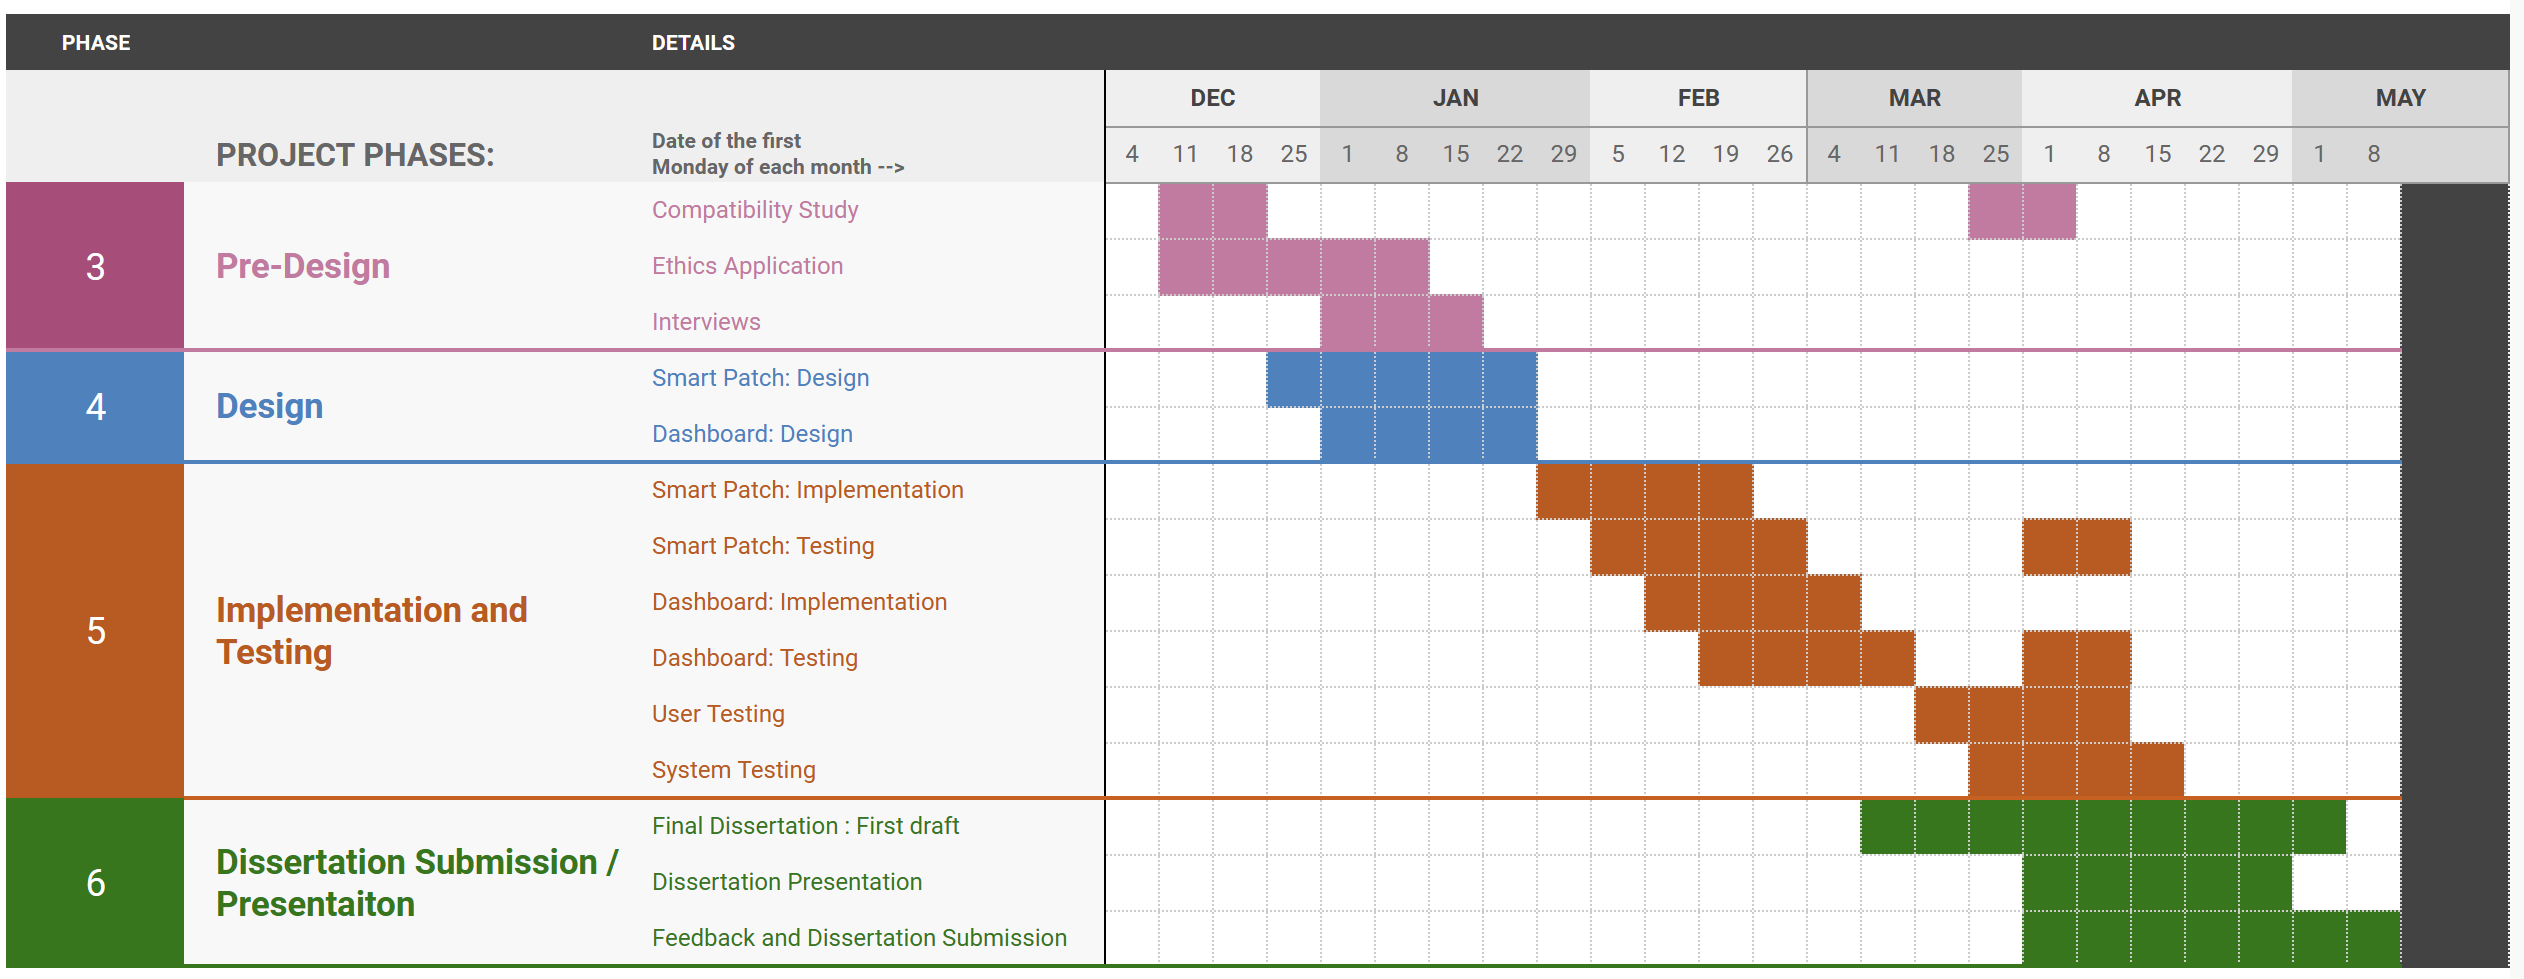
\includegraphics[width=1\linewidth]{images/gantt-chart.png}
        \caption{Project Plan }
        \label{fig:gantt-chart}
    \end{figure}
    
\end{itemize}









\newpage

\chapter{Conclusion}
% Rise in Stress levels in HCPs
% Healthcare Professional's wellbeing
% How IoT and IoTaaS is solving problems in healthcare.
% No solution out there for tracking HCp's wellbeing
% Solution: VitalMonitor
% VitalMonitor being the first solution that caters to HCPs
% Smart Patch being one of the first IoT device to provide remote and non-intrusive healthcare solution
% Implementation
% Evaluation
% Limitations
% Future of VitalMonitor
% Achievements of the project


The healthcare industry has witnessed a significant rise in stress levels among healthcare professionals (HCPs), highlighting the urgent need to prioritize their well-being. Research reveals that the emotional and physical burdens of high-stress environments can profoundly affect HCPs' mental and physical health. Despite significant technological advancements, existing healthcare systems lack comprehensive tools tailored specifically to safeguard the health and well-being of HCPs. This pressing issue calls for a solution that addresses the critical gaps in real-time monitoring and proactive intervention. This led the development of VitalMonitor.\\ \\
VitalMonitor was designed as an innovative system which tackles this problem head-on. At its core is the Smart Patch, one of the first IoT devices specifically engineered to remotely monitor the health of HCPs in a non-intrusive manner. This device measures critical health parameters like heart rate and body temperature, providing real-time insights into stress and fatigue levels. Coupled with an Internet of Things as a Service (IoTaaS) platform, VitalMonitor enables centralized monitoring through a comprehensive web dashboard. The dashboard offers a seamless user experience for healthcare administrators to access health data, generate alerts, and make proactive decisions that help ensure HCPs' safety. \\ \\
A comprehensive literature review revealed the limitations of current healthcare monitoring systems and identified the unique opportunity to fill this void. Existing solutions are primarily focused on patient care and often overlook the well-being of healthcare professionals themselves. This gap prompted the project to develop Smart Patch and web dashboard using an agile methodology. The iterative development process ensured continuous refinement of both the hardware and software components, with thorough testing at each stage.\\ \\
The design phase involved carefully choosing the most suitable technologies, ensuring compatibility between the Smart Patch firmware, middleware, and dashboard components. The ESP32-S3 microcontroller was selected for its built-in wireless connectivity and low power consumption. It was paired with Pimoroni Pulse Sensor and DS18B20 temperature sensor to achieve accurate, non-intrusive monitoring. The middleware used Google Cloud's secure MySQL infrastructure for efficient data management. Finally, the dashboard was built with Python's Flask framework for robust backend support and easy integration.\\ \\ 
The Smart Patch's firmware underwent multiple iterations to enhance its accuracy and reliability. The middleware's API endpoints were rigorously tested to ensure secure data transmission between the device and the dashboard. The dashboard's user interface was designed to prioritize ease of use, allowing administrators to seamlessly monitor HCPs' health metrics in real time. The entire system was subject to unit, integration, and system testing, with special attention to user stories that capture essential functionality. \\ \\ 
VitalMonitor's approach aligns with global health trends, addressing the increasing demand for IoT-based wearable health technology. The system was developed with practical implications in mind, focusing on seamless integration with existing healthcare workflows. This ensures that healthcare organizations can immediately benefit from the system by easily incorporating it into their daily work. \\ \\
While the Smart Patch and dashboard excelled in achieving real-time health monitoring, certain limitations were identified. The system is dependent on network availability, which may impact performance in low-bandwidth environments. Achieving non-intrusive sensor accuracy remains a challenge, necessitating the use of different algorithms such as Moving Average. However, these challenges also present opportunities for future enhancement. By refining middleware infrastructure, implementing prediction models for stress and fatigue, and improving sensor technology through interdisciplinary collaboration, the system's reliability and usability can be further improved.\\ \\
VitalMonitor has the potential to become a leading tool in redefining healthcare monitoring systems. Its proactive approach can significantly impact global healthcare delivery by reducing HCP burnout and ensuring patient safety. The project serves as a testament to the innovation and dedication that went into creating this solution, opening the door to future research and collaboration to improve HCP well-being further. Healthcare organizations, researchers, and developers should consider adopting or building upon VitalMonitor to advance healthcare technology that protects those who protect us all. 
% \newpage
\textbf{Body Placement}

Where exactly should this device be placed?

Why is it important?

Non-Intrusivity and Accuracy

Non-Intrusivity - doesn't bother them while doing an important work
Places where it can be non-intrusive - back of neck/shoulders, behind ears, ankles

Places where we can measure body heart rate using pimoroni pulse sensor
-- 3d body image where all the places are marked

Places where we can measure body temperature using LM-35 sensor
--  3d body image where all the places are marked




\printbibliography[heading=bibintoc, title={Bibliography}]
% \bibliographystyle{ieeetr}
% \bibliography{mybibliography}

\begin{appendices}
\chapter{Stress and Fatigue Level}
\section{Stress Level:}
Stress is a complex physiological and psychological response to external pressures or demands, commonly experienced in high-stress environments such as healthcare settings. Measuring stress levels involves assessing the body's reaction to stressors, which can manifest in various ways, including changes in heart rate, hormonal balance, and nervous system activity. The challenge lies in quantifying stress in real-time due to its multifaceted nature.\\
\section{Fatigue Level:}
Fatigue, often synonymous with tiredness, is a state of extreme tiredness or exhaustion, that impacts both physical and mental capacities. In healthcare professionals working in demanding environments, fatigue can compromise decision-making abilities, reaction times, and overall performance. Like stress, fatigue is a nuanced parameter that requires a comprehensive understanding of physiological and psychological factors.
\chapter{Software Development Lifecycle (SDLC)}
\label{app:agile}

Agile Methodology is a popular approach in SDLC that emphasizes flexibility, collaboration and customer satisfaction \cite{30} \cite{31}. The development process is broken down into sprints (small, incremental builds or iterations). Such an iterative process allows developers to focus on the most important features at any given moment, rather than strictly following a pre-defined plan. \\

Agile Methodology is guided by its four core values \cite{32}: 
\begin{enumerate}
    \item \textbf{Individuals and interactions} over processes and tools
    \item \textbf{Working software} over comprehensive documentation
    \item \textbf{Customer Collaboration} over contract negotiations
    \item \textbf{Responding to change} over following a plan 
\end{enumerate}


\begin{figure}
    \centering
    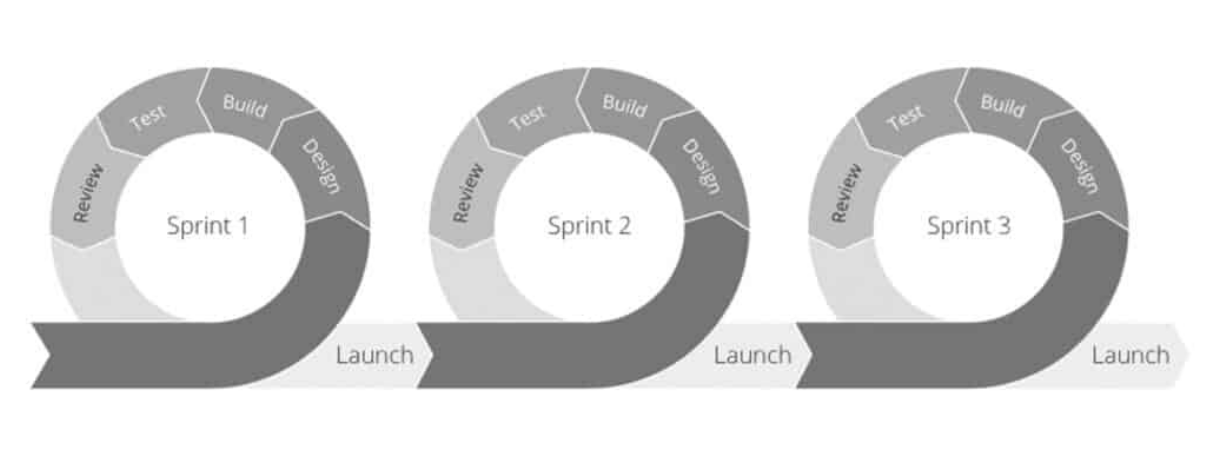
\includegraphics[width=1\linewidth]{images/sdlc.png}
    \caption{Anatomy of Agile Approach \cite{33}}
    \label{fig:sdlc}
\end{figure}



The adoption of this methodology especially in IoT and software development has been widespread for several reasons. 
\begin{itemize}
    \item \textbf{IoT:} Agile methodologies support multiple protocols and networks utilised for building IoT solutions. It enables closer cooperation between IoT hardware and software development teams, fostering higher transparency \cite{30}. This approach successfully addresses the complexity of connecting culture and technology in IoT implementation \cite{34}.
    \item \textbf{Software Development:} As per the 16th State of Agile Report by digital.ai, 78\% of the respondents report that they have implemented or are planning to implement Agile at scale. Agile’s emphasis on building working software quickly fostering cross-functional teams empowered to make decisions, and focusing on rapid iteration with continuous customer input are some of the reasons for its widespread adoption \cite{35}.  This approach not only follows better collaboration and incremental delivery but also provides early error detection and elimination of unnecessary work. 
\end{itemize}



\noindent Looking at the benefits of this approach, this project follows a similar approach. 

\chapter{Features of the System}
\label{app:features}

\begin{itemize}
    \item \textbf{Categorizing the Features} \\
    All the features of the system are categorized into functional and non-functional features.
    \begin{itemize}
        \item \textbf{Functional Features} \\
    Functional features represent the capabilities and behaviours of a system that directly contribute to its primary purpose and functionality. These features are concerned with what the system does and how well it performs its intended tasks.

        \item \textbf{Non-Functional Features} \\
    Non-functional features, on the other hand, are characteristics of a system that do not directly relate to its specific functionalities but rather focus on how well the system performs its functions. 
    
    \end{itemize}
     	
    \item \textbf{MoSCoW Prioritisation FrameWork}\\
    After categorizing features into functional and non-functional, they are prioritized using the MoSCoW Prioritisation FrameWork. The key for this prioritisation is given in Table \ref{tab:key-to-features}.

    \end{itemize}

    \begin{table}[h]
        \centering
        \begin{tabularx}{\textwidth}{|p{3cm}|X|}
            \hline
             \textbf{Category} 
             & \textbf{Description} \\ \hline

             \textbf{Must-Have} 
             & This category consists of features that are “must” for the system. They represent non-negotiable needs for the system.  
             \\ \hline

             \textbf{Should-Have} 
             & 	They are essential for the system, but they are not vital. If left out, the system still functions. However, the features  may add significant value. 
             \\ \hline

             \textbf{Could-Have} 
             & These features are not necessary to the core function of the system. 
             \\ \hline

             \textbf{Won't-Have} 
             & This category contains features which will not be included in a specific release, time frame or prioritised in the future. Their absence is not detrimental to the functionality of the final product.
             \\ \hline

             
        \end{tabularx}
        \caption{Key to features}
        \label{tab:key-to-features}
    \end{table}


\section{Features of Smart Patch}
\subsection{Functional Features}

\begin{table}[h]
    \centering
    \begin{tabularx}{\textwidth}{|p{3cm}|X|p{2cm}|}

         \hline

         \textbf{Feature}
         & \textbf{Description}
         & \textbf{MoSCoW Priority} \\ \hline

         Real-time Monitoring
         & Continuously monitors vital signs (HRV and body temperature) in real-time, providing instant feedback on the wearer's physiological status.
         & Must-Have \\ \hline

         Heart Beat Rate Monitoring
         & Monitor heart bear rate of the wearer in real-time.
         & Must-Have \\ \hline

         Body Temperature Monitoring
         & Monitors body temperature of the wearer in real-time.
         & Must-Have \\ \hline

         Wireless Connectivity 
         & Equipped with wireless capabilities to securely transmit data to a cloud platform, enabling remote access for healthcare institutions.
         & Must-Have \\ \hline
         
    \end{tabularx}
    \caption{Functional Features of Smart Patch}
    \label{table:functional-sp}
\end{table}

\newpage
\subsection{Non-Functional Features}

\begin{table}[h]
    \centering
    \begin{tabularx}{\textwidth}{|p{3cm}|X|p{2cm}|}

         \hline

         \textbf{Feature}
         & \textbf{Description}
         & \textbf{MoSCoW Priority} \\ \hline

        Non-Intrusiveness
        & Designed to be comfortable for prolonged wear, lightweight, unobtrusive, and adhering to safety and hygiene standards. Placed on the body where least intrusive for healthcare professionals.
        & Must-Have \\ \hline

        Device Portability
        & Designed to be easily portable, allowing healthcare professionals to move freely and perform their duties without hindrance.
        & Must-Have \\ \hline

        Regulatory Compliance
        & Adheres to relevant healthcare and IoT regulatory standards to ensure the device's safety, effectiveness, and compliance with legal requirements.
        & Must-Have \\ \hline

        Long Battery Life
        & Designed with a long-lasting battery to minimise the need for frequent recharging, ensuring continuous monitoring during extended shifts.
        & Should-Have \\ \hline

        Durability
        & Constructed with durable materials to withstand daily wear and tear in a healthcare environment, ensuring the device's longevity and reliability.
        & Should-Have \\ \hline

        Compatibility
        & Ensures compatibility with various body types and sizes, accommodating diverse healthcare professionals with different preferences and needs.
        & Should-Have \\ \hline
 
    \end{tabularx}
    \caption{Non-Functional Features of Smart Patch}
    \label{tab:non-functional-sp}
\end{table}






\newpage
\section{Features of Dashboard}

\subsection{Functional Features}

\begin{table}[h]
    \centering
    \begin{tabularx}{\textwidth}{|p{3cm}|X|p{2cm}|}

         \hline

         \textbf{Feature}
         & \textbf{Description}
         & \textbf{MoSCoW Priority} \\ \hline

         Real-time Monitoring
         & Displays real-time heart rate and body temperature data of HCPs, allowing institutions to track vital signs continuously.
         & Must-Have \\ \hline

         Alerts and Threshold
         & Enables institutions to set and receive alerts when an HCP's vital signs surpass predefined thresholds, facilitating timely intervention in case of abnormal patterns.
         & Must-have \\ \hline

         Multiple HCP Tracking 
         & Supports simultaneous monitoring of multiple HCPs, providing a comprehensive overview of the health status of all professionals working at a given time.
         & Should-Have \\ \hline

         User Authentication
         & Implements secure user authentication to ensure authorized access, maintaining the confidentiality and integrity of healthcare data.
         & Could-Have \\ \hline

         Customizable User Permissions
         & Provides customizable user permissions, allowing institutions to control access levels for different roles, ensuring data privacy and security compliance.
         & Could-Have \\ \hline


         
    \end{tabularx}
    \caption{Functional Features of Dashboard}
    \label{table:functional-db}
\end{table}


\newpage
\subsection{Non-Functional Features}

\begin{table}[h]
    \centering
    \begin{tabularx}{\textwidth}{|p{3cm}|X|p{2cm}|}

         \hline

         \textbf{Feature}
         & \textbf{Description}
         & \textbf{MoSCoW Priority} \\ \hline

         User-Friendly Interface
         & Designs an intuitive and user-friendly dashboard interface, enhancing the overall experience for healthcare professionals and administrators interacting with the monitoring system.
         & Must-Have \\ \hline

         Performance Optimisation
         & Optimizes the dashboard's performance to handle real-time data efficiently, ensuring a smooth and responsive user experience even during periods of high data traffic.
         & Should-Have \\ \hline

         Scalability
         & Designs the dashboard to be scalable, accommodating potential future expansions in the number of monitored healthcare professionals without compromising performance or user experience.
         & Should-Have \\ \hline

         Security and Compliance
         & Ensure data security by implementing robust measures to protect sensitive healthcare information, complying with relevant regulations and industry standards.
         & Should-Have \\ \hline

    \end{tabularx}
    \caption{Non-Functional Features of Dashboard}
    \label{table:non-functional-db}
\end{table}
\chapter{Legal Considerations}

\section{Data Protection Regulations}

The healthcare sector extensively employs information technologies, including wearable health monitoring devices and IoT (Internet of Things) devices, for real-time vital monitoring and data collection. These technologies involve the processing of significant amounts of personal data, necessitating adherence to data protection regulations. \\ \\
Within the European Union (EU), personal data processing in healthcare is regulated by the General Data Protection Regulation (GDPR), which came into effect on May 25, 2018. The GDPR mandates obligations for data controllers and processors, ensuring the protection of individuals' personal data. Developers and providers of healthcare IoT devices must formulate privacy policies that align with GDPR requirements to ensure compliance.

\section{Medical Regulations}

Regulatory oversight in the UK for medical devices and IoT devices in healthcare is managed by the Medicines and Healthcare products Regulatory Agency (MHRA). Medical devices, including IoT devices used for vital monitoring, are categorized based on risk levels, ranging from low risk (Class I) to high risk (Class III). Even low-risk devices are subject to regulatory requirements, such as documentation preparation, clinical evaluations, and post-production review procedures. IoT devices intended for vital monitoring purposes fall under the scope of medical device regulations. Manufacturers must adhere to MHRA guidelines, which may include obtaining certifications and conducting clinical evaluations. \\ \\
In compliance with regulatory guidelines, it is essential for developers and providers of IoT devices for vital monitoring to ensure transparency and accountability in data processing practices. Users should be informed about data collection processes and their rights regarding their personal data.


\chapter{Ethical Considerations}

In deploying IoT (Internet of Things) devices for passive monitoring in healthcare, several ethical considerations must be taken into account to ensure responsible and ethical use of technology.
\begin{itemize}
    \item Ensuring data privacy and confidentiality is paramount, even in passive monitoring scenarios. Measures such as encryption, secure data transmission protocols, and access controls should be implemented to protect the confidentiality of collected data.
    \item While passive monitoring may not require active patient participation, it's essential to inform individuals about the presence and purpose of monitoring devices. Transparency about data collection activities helps build trust and respect for individuals' autonomy, even if explicit consent is not obtained.
    \item Clarifying data ownership and control is important, particularly regarding the rights and responsibilities of data stewards. Individuals should have clarity on who has access to their data and how it will be used, with mechanisms in place for individuals to access, modify, or delete their data as needed.
    \item In cases where algorithms are used to analyze collected data, transparency in algorithmic processes is crucial. Individuals should have visibility into how algorithms operate and make decisions to ensure accountability and mitigate risks of bias or discrimination.
    \item Consideration of the broader social implications of passive monitoring is essential. While these technologies offer potential benefits in terms of healthcare optimization, they may also raise concerns about surveillance and privacy infringement. 
\end{itemize}

\noindent For the entire development and testing stage, it is advisable to utilize solely the developer's own health data rather than actual human health data to ensure ethical and responsible practices.

\chapter{Sensors}
To understand how sensors work, this section provides an overview of the colour coding of the sensors and the circuit diagram of each sensor used in the project.

\begin{figure}
    \centering
    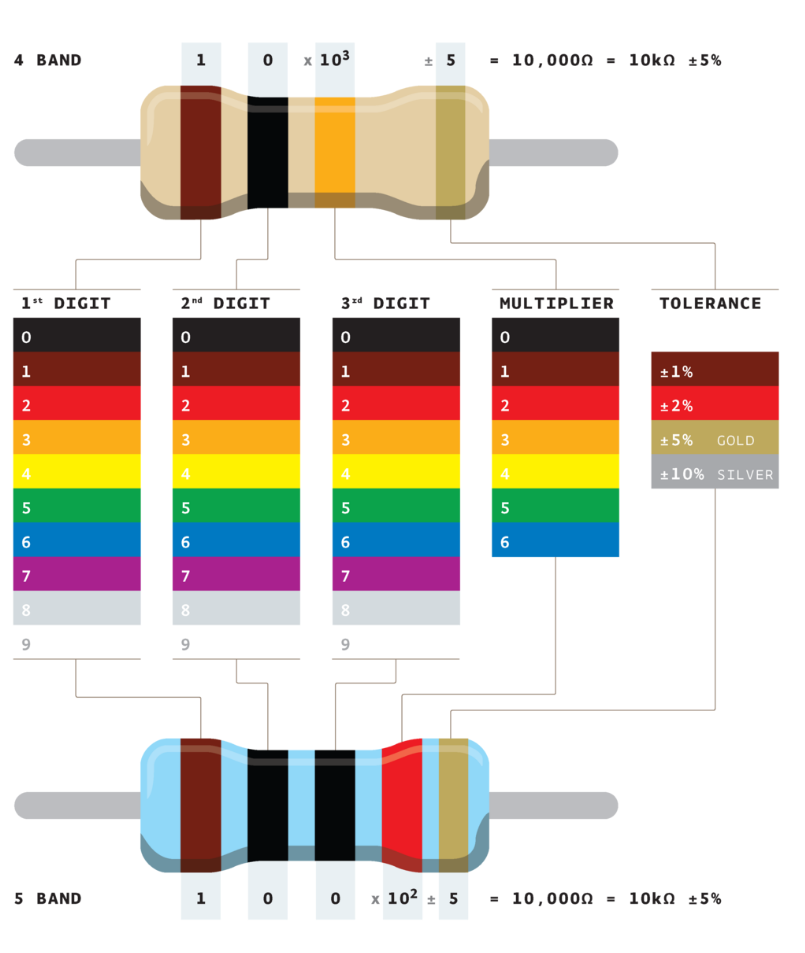
\includegraphics[width=0.5\linewidth]{images/sensors-color-code.png}
    \caption{ Colour codes in sensors \cite{36}}
    \label{fig:sensors-color-code}
\end{figure}

\section{Pulse Sensor Circuit}
Figure \ref{fig:pulse-sensor} shows the internal circuit diagram of a pulse sensor. It consists of an optical heartbeat sensor, an amplification circuit, and a noise cancellation circuit.

\begin{figure}
    \centering
    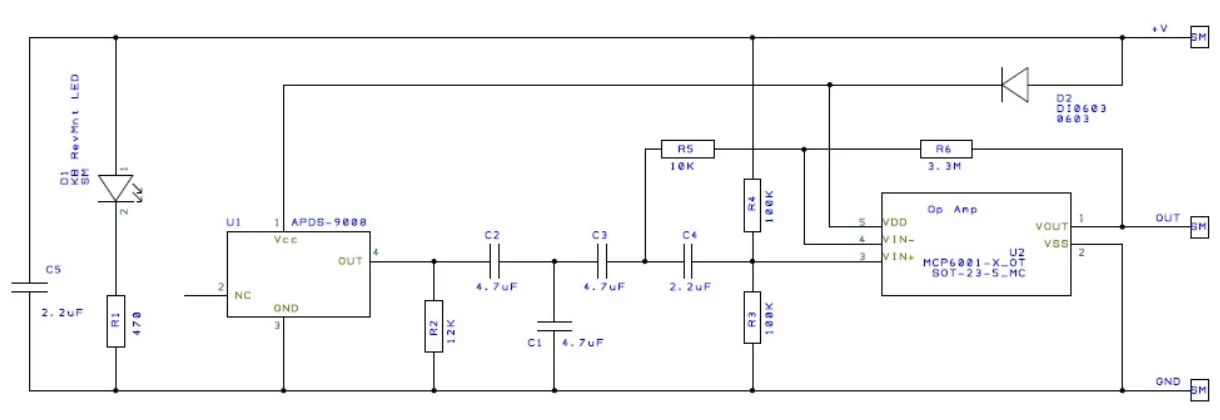
\includegraphics[width=0.75\linewidth]{images/image.png}
    \caption{Internal block diagram of an SEN-11574 pulse sensor \cite{37}}
    \label{fig:pulse-sensor}
\end{figure}

\section{LM-35 Sensor Circuit}
Figure \ref{fig:lm-35-sensor} shows the internal circuit diagram of a LM-35 sensor. In the figure, A1 shows the input where it senses the temperature and A2 provides the output voltage of the circuit. The circuit is made in such a way that it outputs a voltage proportional to the temperature it measures. This makes it easier to calculate the temperature of body eliminating electronic complexities. 

\begin{figure}
    \centering
    \includegraphics[width=0.5\linewidth]{images/lm-35.png}
    \caption{Internal block diagram of IC LM-35 Sensor \cite{38}}
    \label{fig:lm-35-sensor}
\end{figure}

\chapter{Similar Software Available for IoT Development}

A number of softwares are available in the market for free of cost which supports IoT development. Below are some of the most commonly-used software for such development. If in the later phases of the project, it is find that it is efficient to use these instead of native development, they will be adopted.

\begin{enumerate}
    \item \textbf{The Things Network (TTN)}\\
	Used: IoT cloud platform\\
TTN is an open-source, decentralized infrastructure dedicated to IoT. TTN uses LoRaWAN as its secure messaging protocol. Devices that support LoRa can connect to gateways scattered all around the world that bridge them with TTN. It enables community users to create applications for data viewing and interact with the service by sending data from other IoT devices to other registered devices and gateways.

\item \textbf{ThingsBoard}\\
	Used: Dashboard tool\\
ThingsBoard is an open-source IoT platform for data collection, processing, visualization, and device management. It enables device connectivity via industry standard IoT protocols - MQTT, CoAP and HTTP and supports both cloud and on-premises deployments. The benefits of using ThingsBoard are scalability, fault-tolerance and performance so that data is intact. \cite{39}

\item \textbf{ThingSpeak}\\
Used: Analysis and Visualization\\
For even more advanced functionalities, there is ThingSpeak which is an IoT analytics platform service. This service allows a user to aggregate, visualize and even analyse live data streams without having to write any code. What makes ThingSpeak special is that it supports MATLAB analytics functions; users can write and run MATLAB code for more advanced analyses. ThingSpeak can also integrate with TTN to retrieve data from connected devices. \cite{40}

\item \textbf{Adafruit IO}\\
Used: IoT cloud platform\\
Adafruit IO is a cloud service. It can display data online from sensors in real-time, and connect to devices and control components. With a dashboard creator feature built-in, the software is capable of handling and visualizing multiple feeds of data. Adafruit IO can also be integrated with applications such as IFTTT and Zapier and other web services such as Twitter, RSS feeds etc. \cite{41}
\end{enumerate}
\chapter{Risk Analysis}

This chapter lists down all the potential risks that this project might face. The risk register provided in Figure \ref{fig:rr} is continuously updated throughout the project timeline as per the key to risk rating provided in Figure in \ref{fig:ktrr}.

\vspace{5.5cm}
\noindent\textbf{Key to Risk Rating:}
\begin{figure}
    \centering
    \includegraphics[width=1\linewidth]{images/ktrr.png}
    \caption{Key to Risk Rating}
    \label{fig:ktrr}
\end{figure}

\begin{figure}
    \centering
    \includegraphics[width=1\linewidth]{images/rr.png}
    \caption{Risk Register}
    \label{fig:rr}
\end{figure}
\chapter{Adafruit IO Dashboard}
\label{app:adafruit}

Adafruit IO Dashboard was integrated with the system 
Integration with Adafruit IO is achieved through the MQTT protocol, where the device publishes sensor data to specific feeds. The corresponding dashboard on Adafruit IO is configured to subscribe to these feeds, thereby enabling real-time monitoring of health data.


\subsection{Use of MQTT Protocol}
To handle real-time communication and data transmission from Smart Patches to Adafruit IO Dashboard, MQTT (Message Queuing Telemetry Transport) protocol is used. MQTT is chosen for its lightweight nature and effectiveness in scenarios requiring minimal network bandwidth and device power consumption, which are critical in IoT contexts. Devices publish data to specific topics, which are dynamically subscribed to Adafruit IO Dashboard by the backend, enabling flexible and decoupled communication strategies.


--- ADD DIAGRAM FOR MQTT PROTOCOL
\chapter{Manual Testing}
\label{app:manual-testing}
\begin{longtable}{|c|p{6cm}|p{4cm}|c|}
\caption{Manual Test Cases for VitalMonitor Web Dashboard} \label{tab:manual_tests_web} \\
\hline
\textbf{Test Case ID} & \textbf{Test Details} & \textbf{Expected Results} & \textbf{Pass/Fail} \\
\hline
\endfirsthead

\multicolumn{4}{c}%
{{\bfseries Table \thetable\ Continued from previous page}} \\
\hline
\textbf{Test Case ID} & \textbf{Test Details} & \textbf{Expected Results} & \textbf{Pass/Fail} \\
\hline
\endhead

\hline
\multicolumn{4}{|r|}{{Continued on next page}} \\ \hline
\endfoot

\hline
\endlastfoot

TC-WD01 & Verify that admins can register an organization using valid details. \newline
- Navigate to registration form. \newline
- Input all required fields. \newline
- Submit form. & Admins are taken to home page. & Pass\\
\hline
TC-WD02 & Verify admin login functionality with correct credentials. \newline
- Access login page. \newline
- Enter valid credentials. \newline
- Click login. & Admin is redirected to the dashboard home page. & Pass \\
\hline
TC-WD03 & Verify the addition of a new device. \newline
- Log in as admin. \newline
- Navigate to "Add New Device" page. \newline
- Enter device details and submit. & Device addition confirmation message is displayed. & Pass \\
\hline
TC-WD04 & Verify user-device assignment functionalities. \newline
- Log in and view user list. \newline
- Select a user without a device. \newline
- Assign a device and submit. & Device is listed as assigned to the user. & Pass \\
\hline
TC-WD05 & Check the functionality of logging out. \newline
- Log in to the dashboard. \newline
- Click the logout button. & User is redirected to the login screen and session ends. & Pass \\
\hline
\end{longtable}

\begin{longtable}{|c|p{6cm}|p{4cm}|c|}
\caption{Manual Test Cases for Smart Patch Device} \label{tab:manual_tests_device} \\
\hline
\textbf{Test Case ID} & \textbf{Test Details} & \textbf{Expected Results} & \textbf{Pass/Fail} \\
\hline
\endfirsthead

\multicolumn{4}{c}%
{{\bfseries Table \thetable\ Continued from previous page}} \\
\hline
\textbf{Test Case ID} & \textbf{Test Details} & \textbf{Expected Results} & \textbf{Pass/Fail} \\
\hline
\endhead

\hline
\multicolumn{4}{|r|}{{Continued on next page}} \\ \hline
\endfoot

\hline
\endlastfoot

TC-SP01 & Verify activation of the Smart Patch by pressing the button. \newline
- Ensure the device is off. \newline
- Press the activation button. & Device turns on (red light indicator) and starts transmitting data. & Pass \\
\hline
TC-SP02 & Verify deactivation of Smart Patch by pressing the button again. \newline
- Ensure the device is on. \newline
- Press the button again. & Device turns off (red light off) and stops transmitting data. & Pass \\
\hline
TC-SP03 & Verify continuous data transmission of heart rate and temperature. \newline
- Activate the device. \newline
- Monitor the data transmission for 10 minutes. & Continuous, accurate data transmission is observed. & Pass \\
\hline
\end{longtable}
\chapter{Abbreviations}
AA - Double-A (battery size) \\
BLE - Bluetooth Low Energy\\
BMJ - British Medical Journal\\
CoAP - Constrained Application Protocol \\
GPIO - General Purpose Input/Output\\
HTTP - Hypertext Transfer Protocol\\
HCp - Healthcare Professionals\\
I/O or IO - Input/Output\\
IaaS - Internet of Things as a Service
IC - Integrated Circuit\\
IDE - Integrated Development Environment\\
IDF - IoT Development Framework\\
ICU - Intensive Care Unit\\
IoT - Internet of Things\\
IoMT - Internet of Medical Things\\
IoTaaS - Internet of Things as a service
IVD - In-Vitro Devices\\
LiIon - Lithium-Ion\\
LiPo - Lithium Polymer\\
LoRaWAN - Long Range Wide Area Network\\
MCU - Microcontroller Unit\\
MERN - MongoDB, ExpressJS, ReactJS, NodeJS\\
MQTT - Message Queuing Telemetry Transport\\
NoSQL - Not Only SQL (database)\\
OS - Operating System\\
PPG - Photoplethysmography\\
RAM - Random Access Memory\\
ROM - Read Only Memory\\
SDLC - Software Development Lifecycle\\
TTN - The Things Network\\
USB - Universal Serial Bus\\

\end{appendices}

\end{document}